\documentclass[11pt, a4paper]{scrartcl} % Packages
%\usepackage{stix}
\usepackage{sansiwona}
\usepackage[margin=1.5in]{geometry}
\usepackage{index}
\makeindex
\usepackage[utf8]{inputenc}
\usepackage[T1]{fontenc}
\usepackage{varwidth}
\usepackage{amsmath, amssymb, amsbsy}
\usepackage{esint}
\usepackage{titlesec}
\usepackage{xcolor}
\usepackage{titling}
\usepackage{braket}
\usepackage{tensor}
\usepackage[linktocpage]{hyperref}
\usepackage{pgfplots}
\usepackage{multicol}
\setlength{\columnsep}{2em}
\usepackage{caption}
\usepackage{amsthm}
\usepackage{import}
\usepackage{cancel}
\usepackage{caption}
\usepackage{tcolorbox}
\usepackage{nicematrix}
\usepackage{mathtools}
\usepackage{enumerate}
\usepackage{graphicx}
\usepackage{lipsum}
\usepackage[italian]{babel}
% To reset footnote numbering each page
\usepackage[perpage]{footmisc}
\usepackage{setspace}
\setstretch{1.2}

%Captions
\captionsetup[figure]{font=footnotesize,labelfont=footnotesize}
\captionsetup[table]{font=footnotesize,labelfont=footnotesize}
%Titlesec
\titleformat{\section}
{\fontsize{15}{20}\sffamily\scshape}
{\normalfont\color{gray}{\fontsize{20}{20}\selectfont\thesection}}
{0.7em}
{}
\hypersetup{colorlinks,breaklinks, linkcolor=[RGB]{74, 122, 164}}

\newcommand\vertarrowbox[3][6ex]{%
  \begin{array}[t]{@{}c@{}} #2 \
  \left\uparrow\vcenter{\hrule height #1}\right.\kern-\nulldelimiterspace\
  \makebox[0pt]{\scriptsize#3}
  \end{array}%
}
\definecolor{asdf}{HTML}{4a7aa4}
% Personalizza la formattazione della subsection
\titleformat{\subsection}[block]{\fontsize{13}{20}\bfseries}{\normalfont\thesubsection}{.5em}{}


% Personalizza la formattazione della subsubsection
\titleformat{\subsubsection}[block]{\fontsize{12}{20}\bfseries}{\normalfont\thesubsubsection}{.5em}{}

% Maketitle customization
\renewcommand{\maketitle}{
\begin{center}
{\sffamily
{\fontsize{20}{20}\selectfont\MakeUppercase\thetitle}}

\vspace{0.2in}

{\large\scshape\sffamily\theauthor}
\end{center}
}

% Titles 
\title{Note di\\ \vspace{.1in} Meccanica Quantistica}
\author{Manuel Deodato}
\date{}



%Evaluate symbol
\DeclareMathOperator{\di}{d\!}
\newcommand*\Eval[3]{\left.#1\right\rvert_{#2}^{#3}}

%%%%%%% Numero delle equazioni in formato a.b
\numberwithin{equation}{subsection}
%%%%%

%%%%%%%%%% Personalizzazione numeri lista
\renewcommand{\theenumi}{(\arabic{enumi})}

%%%%%%%%%% Medie con integrali multipli
\def\Yint#1{\mathchoice
    {\YYint\displaystyle\textstyle{#1}}%
    {\YYint\textstyle\scriptstyle{#1}}%
    {\YYint\scriptstyle\scriptscriptstyle{#1}}%
    {\YYint\scriptscriptstyle\scriptscriptstyle{#1}}%
      \!\iint}
\def\YYint#1#2#3{{\setbox0=\hbox{$#1{#2#3}{\iint}$}
    \vcenter{\hbox{$#2#3$}}\kern-.51\wd0}}
\def\longdash{{-}\mkern-3.5mu{-}} 
   % consider using "\mkern-7.5mu" if esint package is loaded
\def\tiltlongdash{\rotatebox[origin=c]{15}{$\longdash$}}
\def\fiint{\Yint\tiltlongdash}

\def\Zint#1{\mathchoice
    {\YYint\displaystyle\textstyle{#1}}%
    {\YYint\textstyle\scriptstyle{#1}}%
    {\YYint\scriptstyle\scriptscriptstyle{#1}}%
    {\YYint\scriptscriptstyle\scriptscriptstyle{#1}}%
      \!\iiint}
      \def\tilongdash{\mkern6mu{-}\mkern-4mu{-}\mkern-5mu{-}} 
   % consider using "\mkern-7.5mu" if esint package is loaded
\def\titiltlongdash{\rotatebox[origin=c]{15}{$\tilongdash$}}
\def\fiiint{\Zint\titiltlongdash}


%%%% Table of contents

\usepackage[titles]{tocloft}

\renewcommand{\cftdot}{}
\usepackage{titletoc}
%\setcounter{tocdepth}{2}

%%%%%%%%%%%%%%%% Toc style

% Personalizzazione scritta indice




% Ambienti
\newtheoremstyle{style1}% name of the style to be used
{15pt}% measure of space to leave above the theorem. E.g.: 3pt
{15pt}% measure of space to leave below the theorem. E.g.: 3pt
{\normalfont}% name of font to use in the body of the theorem
{}% measure of space to indent
{\sffamily\scshape\bfseries}% name of head font
{}% punctuation between head and body
{ }% space after theorem head; " " = normal interword space
{\thmname{#1}\thmnumber{ #2}{\thmnote{~--- #3}}.\newline}

\newtheoremstyle{style2}% name of the style to be used
{15pt}% measure of space to leave above the theorem. E.g.: 3pt
{15pt}% measure of space to leave below the theorem. E.g.: 3pt
{\normalfont}% name of font to use in the body of the theorem
{}% measure of space to indent
{\sffamily\scshape\bfseries}% name of head font
{}% punctuation between head and body
{ }% space after theorem head; " " = normal interword space
{\thmname{#1}\thmnumber{ #2}{\thmnote{~--- #3}}.\ }


\theoremstyle{style2}
\newtheorem{osservazione}{Osservazione}[section]

\theoremstyle{style1}
\newtheorem{teorema}{Teorema}[section]
\newtheorem{corollario}{Corollario}[teorema]
\newtheorem{lemma}{Lemma}[teorema]
\newtheorem{definizione}{Definizione}[section]
\newtheorem{notazione}{Notazione}[section]
\newtheorem{esempio}{Esempio}[section]
\newtheorem{esercizio}{Esercizio}[section]

\renewcommand\qedsymbol{$\blacksquare$}

\newenvironment{svolgimento}{\renewcommand\qedsymbol{$\spadesuit$}\begin{proof}[Svolgimento]}{\end{proof}}

%% Generic box
\newtcolorbox{eqbox}[1][]
{
colback=gray!10,
arc=0pt,
boxrule=0pt,
title=#1
}

 \newenvironment{boxenv}[1][]{
    \begin{eqbox}[#1]
    }{
   \end{eqbox}
}






% Font
\usepackage[osf]{newpxtext}
\usepackage{newpxmath}
\usepackage{cmupint}
%%%


%%%%%%%%%%%%%%%%%%%%%%%%%%%%%%%%%%%%%%%%%%%%%%%%%%%%%%%%%%%%%%%%%%%%%%%%

\begin{document}
\maketitle
\vspace{25em}
\begin{figure}[h!]
	\centering
	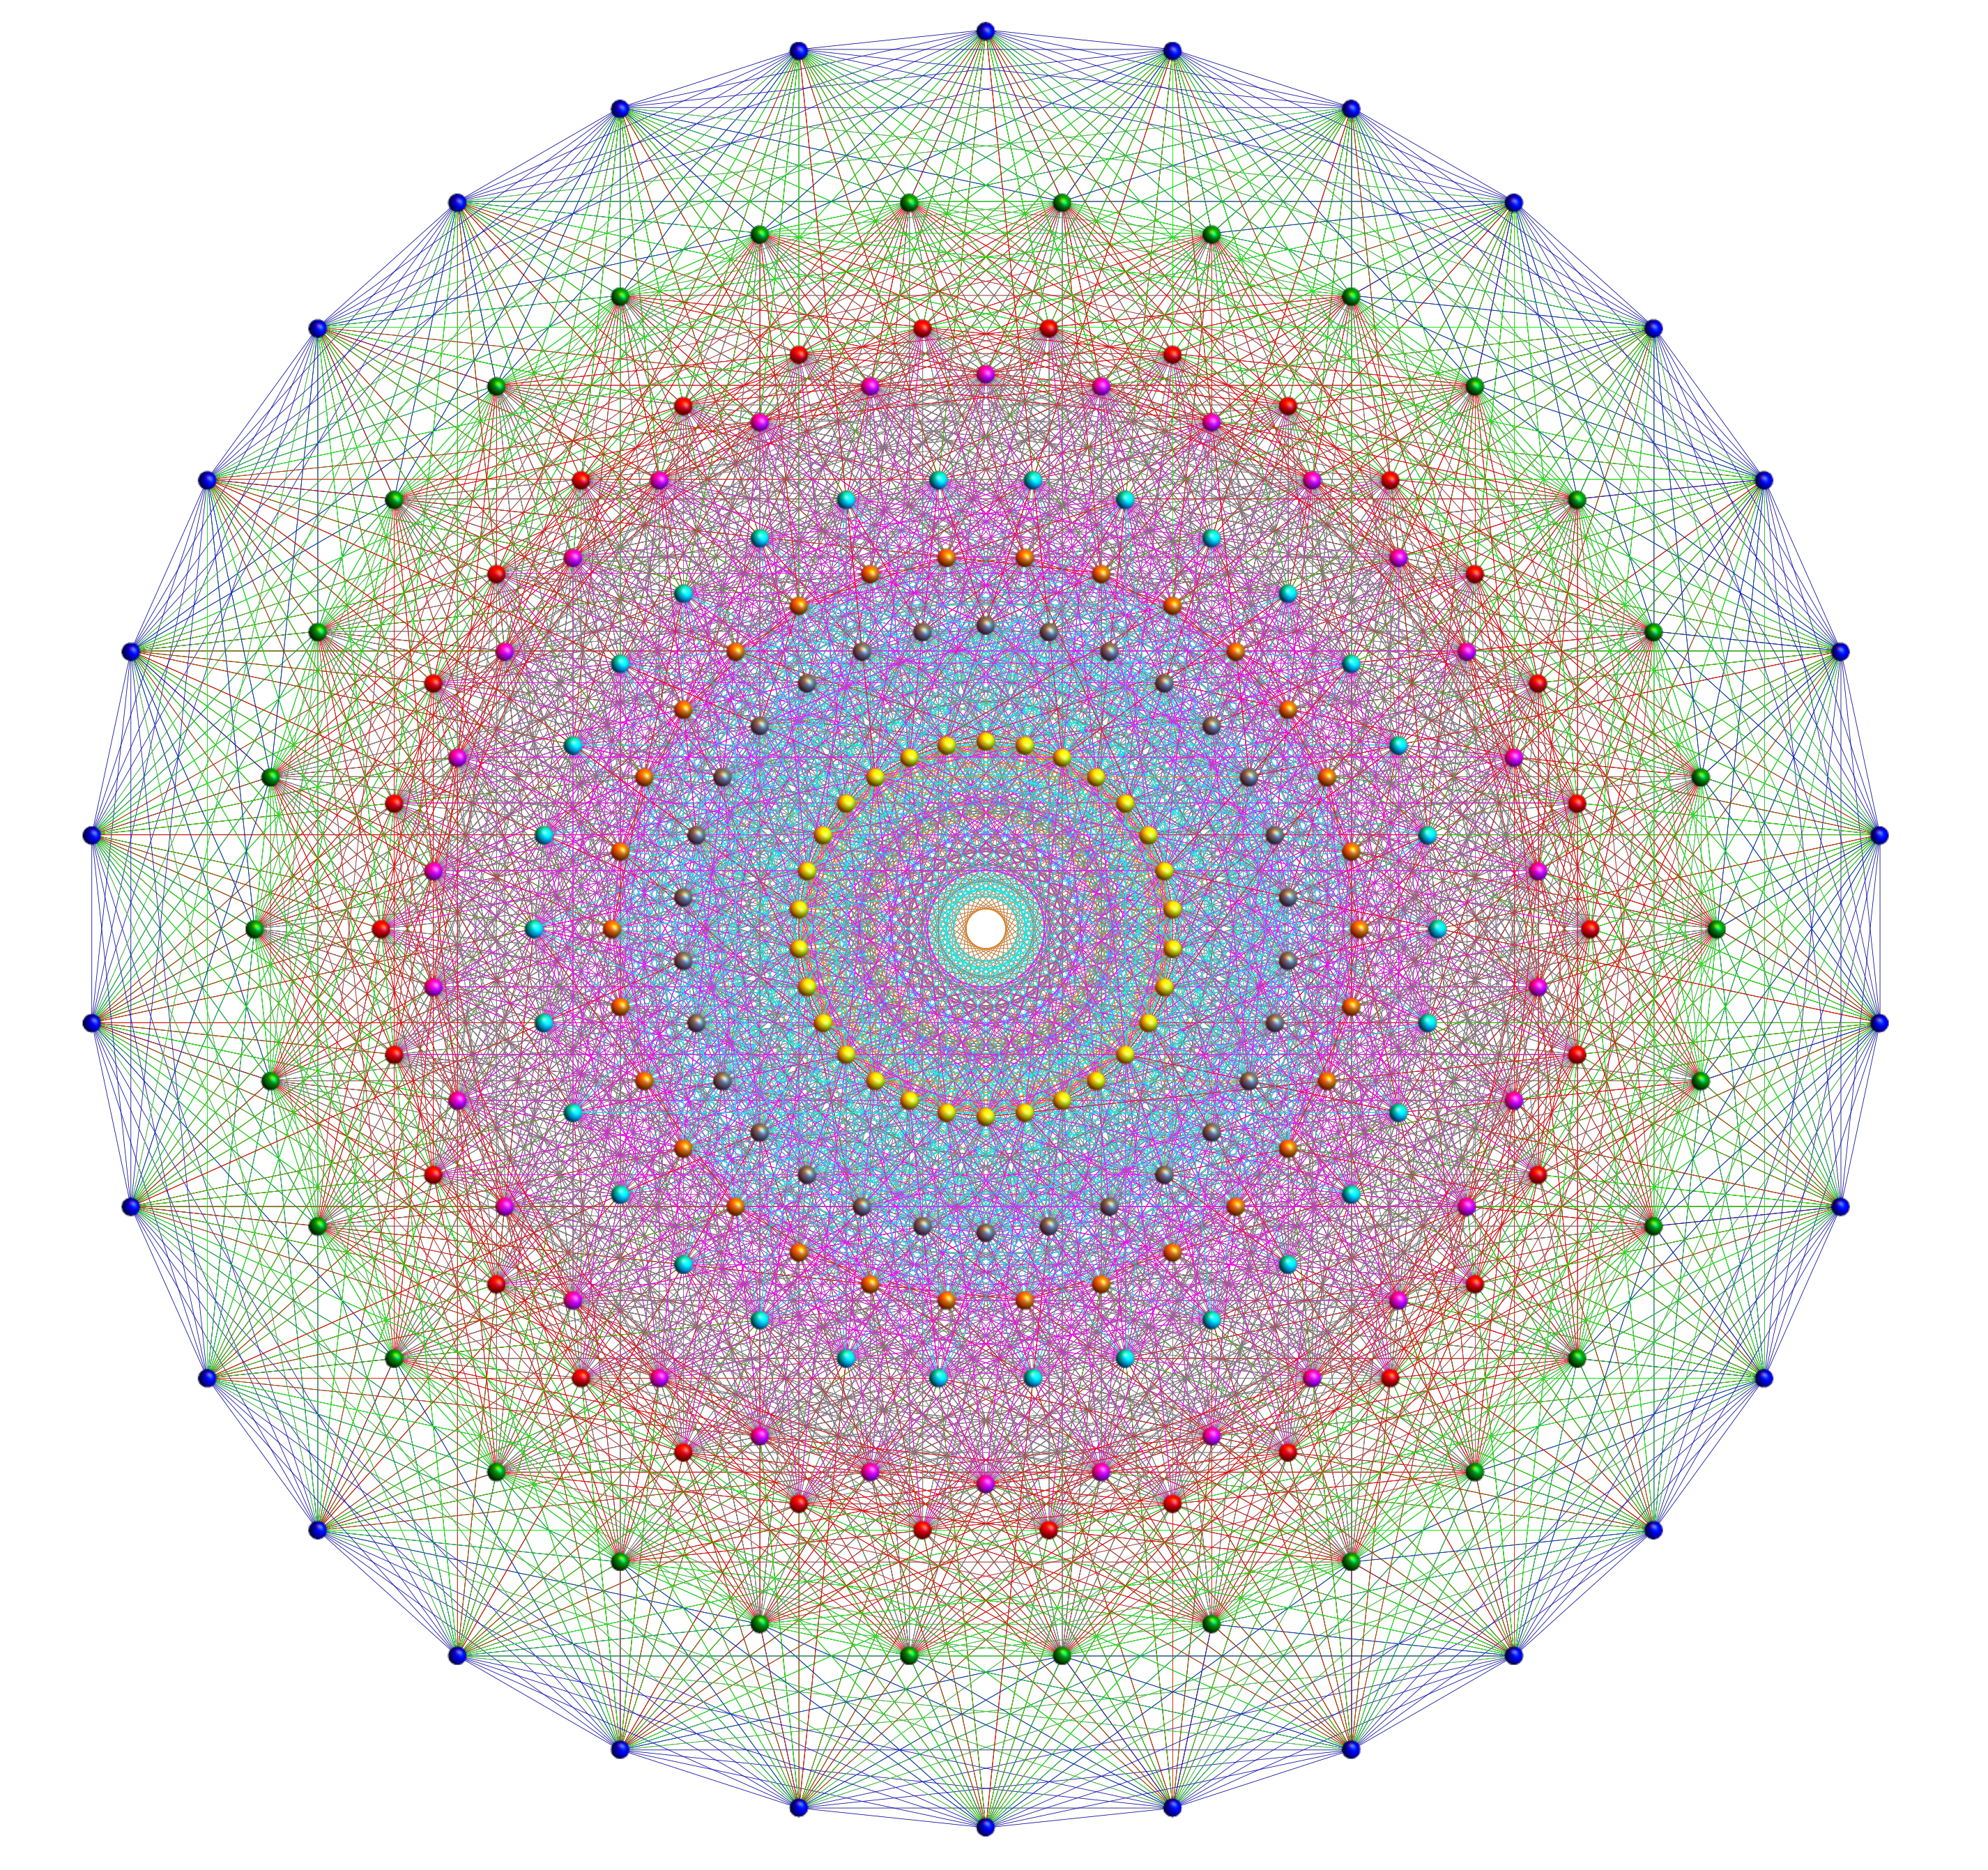
\includegraphics[width=1\columnwidth]{front.jpg}
\end{figure}
\newpage
\tableofcontents 
\newpage
\section{Struttura matematica della meccanica quantistica}
\subsection{Introduzione}
\begin{definizione}
	[Prodotto scalare]
	Per $V$ spazio vettoriale su $\mathbb{C}$ e $\psi ,\phi \in V$, si definisce $\left\langle \cdot ,\cdot  \right\rangle : V\times V \to \mathbb{C}$ come:
	\begin{itemize}
		\item $\left\langle \psi ,\phi  \right\rangle\in \mathbb{C}$;
		\item $\left\langle \psi ,\phi  \right\rangle= \left\langle \phi ,\psi  \right\rangle^*$;
		\item $\left\langle \psi, c_1\phi_1 + c_2\phi_2 \right\rangle = c_1\left\langle \psi ,\phi_1 \right\rangle + c_2 \left\langle \psi , \phi_2 \right\rangle$, con $c_1,c_2 \in \mathbb{C}$;
		\item $\left\langle \phi ,\phi  \right\rangle\ge 0$ e $\left\langle \phi ,\phi  \right\rangle=0 \iff \phi =0$.
	\end{itemize}
\end{definizione}
\noindent Dato $\phi \in V$, questo induce la \textbf{norma}:
\begin{equation}
	\left\lVert \phi  \right\rVert \overset{\text{def}}{=} \sqrt{\left\langle \phi ,\phi  \right\rangle} 
\end{equation}
Si ricordano le seguenti disuguaglianze:
\begin{equation}
	\begin{split}
		&\text{\textbf{Schwarz}: } \left\lvert \left\langle \phi ,\psi  \right\rangle \right\rvert ^2 \le  \left\langle \phi ,\phi  \right\rangle\left\langle \psi ,\psi  \right\rangle\\
		&\text{\textbf{Triangolare}: } \left\lVert \phi + \psi  \right\rVert \le  \left\lVert \psi  \right\rVert +\left\lVert \phi  \right\rVert 
	\end{split}
\end{equation}
\begin{teorema}
	[Teorema di Riesz]
	Dato $T$ operatore lineare limitato agente su spazio di Hilbert $\mathcal{H}$, allora $\exists f \in \mathcal{H}:\forall \phi \in \mathcal{H}\Rightarrow T(\phi )\equiv \left\langle f,\phi  \right\rangle$. Inoltre, $\left\lVert T \right\rVert = \left\lVert f \right\rVert $.
\end{teorema}
\begin{osservazione}
	[Funzionali e operatori]
	Un funzionale lineare \`e un operatore lineare $F$ che agisce su uno spazio vettoriale $V$ su $\mathbb{K}$ e restituisce un valore nel campo; formalmente: $F:V\to \mathbb{K}$. In generale, gli operatori non restituiscono valori in $\mathbb{K}$, mentre i funzionali s\`i.	

Gli operatori rappresentano gli osservabili, mentre i funzionali sono usati per calcolare aspettazione e probabilit\`a.
\end{osservazione}
\subsubsection{Notazione bra-ket}
Sia $V$ uno spazio vettoriale e $V'$ il suo duale; si definiscono:
\begin{itemize}
	\item per $\phi \in V \longrightarrow \ket{\phi } \in V$;
	\item per $F \in  V' \longrightarrow \bra{F} \in V'$.
\end{itemize}
Per Riesz, per qualche $f \in V$:
\begin{equation}
	\braket{F|\phi } \overset{\text{def}}{=}F(\phi ) = \left\langle f,\phi  \right\rangle \Rightarrow F(\phi ) \leftrightarrow \braket{f|\phi}
\end{equation}
Visto che $\braket{\phi |\psi } = \left\langle \phi ,\psi  \right\rangle$, allora: 
\begin{equation}
	\bra{c\phi } = c^* \bra{\phi } \longleftrightarrow \ket{c\phi } = c \ket{\phi } 
\end{equation}
\subsubsection{Operatori}
Si considerano vettori, o \textbf{stati}, in uno spazio di Hilbert $\mathcal{H}$. Un operatore che agisce su tale spazio \`e definito come $\hat{A}: \mathcal{H}\to \mathcal{H}$, quindi $\hat{A}\ket{\phi } \in \mathcal{H}$. Gli operatori di interesse saranno \textbf{lineari}.

Se $\hat{A}$ \`e limitato (quindi continuo), dato $\ket{\psi } \in \mathcal{H}$, con $\left\{ \phi _i \right\} $ base ortonormale:
\begin{equation*}
	\begin{cases}
		 \hat{A}\ket{\psi } = \ket{\phi } = \sum_{i=1}^{+\infty} c_i \ket{\phi _i}  \\
		\\
		 \hat{A}\ket{\psi } = \sum_{i=1}^{+\infty} b_i \hat{A}\ket{\phi _i} 
	\end{cases}
\end{equation*}
si nota che
\begin{equation}
	\braket{\phi _j|\hat{A}\psi } =\bra{\phi _j} \left(\sum_{i=1}^{+\infty} b_i \hat{A} \ket{\phi _i} \right)  = \sum_{i=1}^{+\infty} b_i\underbracket{\braket{\phi _j|\hat{A}|\phi _i}}_{\equiv A_{ji} } 
\end{equation}
dove $A_{ji} $ \`e un elemento di matrice; infatti
\begin{equation*}
		 \braket{\phi _j|\phi } = \braket{\phi _j|\hat{A}|\psi } = \sum_{i=1}^{+\infty}c_i \braket{\phi _j|\phi _i} = c_j
\end{equation*}
da cui, unendo le uguaglianze:
\begin{equation*}
\sum_{i=1}^{+\infty} A_{ji} b_i = c_j	
\end{equation*}
Sia $\hat{A}$ lineare; l'aggiunto \`e $\hat{A}^\dagger $ e tale che $\langle \phi , \hat{A}\psi  \rangle= \langle \hat{A}^\dagger \phi ,\psi  \rangle$. Allora, in notazione bra-ket:
\begin{equation}
	\bra{w} = \bra{\phi } \hat{A}^\dagger \longleftrightarrow \ket{w} = \hat{A}\ket{\phi } 
\end{equation}
Inoltre 
\begin{boxenv}[]
\begin{equation}
	\begin{split}
		&\left\langle \psi ,\phi  \right\rangle^* = \left\langle \phi ,\psi  \right\rangle \implies \braket{\psi |\phi } ^* = \braket{\phi |\psi }\\
		& \Rightarrow \braket{\psi  |\hat{A}^\dagger |\phi } ^* = \braket{\phi |\hat{A}|\psi } 
	\end{split}
\end{equation}
\end{boxenv}
\noindent Infine, se $\left\{ \phi _i \right\} $ base ortonormale:
\begin{boxenv}[]
\begin{equation}
	A^\dagger _{ij} = \braket{\phi _i|\hat{A}^\dagger |\phi _j} = \braket{\phi _j|\hat{A}|\phi _i} ^* = A_{ji} ^* \Rightarrow A^\dagger = (A^\top)^*
\end{equation}
\end{boxenv}
\noindent Da questo, segue:
\begin{equation}
	(AB)^\dagger = B^\dagger A^\dagger; \ (cA)^\dagger = c^* A^\dagger 
\end{equation}
\subsubsection{Operatori autoaggiunti}
\begin{definizione}
	[Operatore autoaggiunto]
	Sia \( \mathcal{H} \) uno spazio di Hilbert complesso e sia \( A \) un operatore lineare definito su un dominio \( \operatorname{Dom} (A) \subseteq \mathcal{H} \). L'operatore \( A \) si dice \textbf{autoaggiunto} se soddisfa le seguenti condizioni:

\begin{enumerate}
    \item \textbf{Densità del dominio:} il dominio \( \text{Dom}(A) \) è denso nello spazio di Hilbert \( \mathcal{H} \), ovvero:
    \[
    \overline{\text{Dom}(A)} = \mathcal{H}.
    \]

    \item \textbf{Simmetria:} per ogni \( \psi, \phi \in \text{Dom}(A) \),
    \[
    \langle \psi, A \phi \rangle = \langle A \psi, \phi \rangle.
    \]

    \item \textbf{Uguaglianza con l'aggiunto:} il dominio di \( A \) coincide con quello del suo aggiunto \( A^\dagger \), e i due operatori coincidono, ovvero:
    \[
    \text{Dom}(A) = \text{Dom}(A^\dagger) \quad \text{e} \quad A = A^\dagger.
    \]
\end{enumerate}
\end{definizione}
\noindent Essendo $\hat{A}= \hat{A}^\dagger $, si ha $A_{ij} = (A_{ij} ^*)^\top$. Questi sono sempre diagonalizzabili, quindi hanno base ortonormale di autovettori. Visto che $\braket{\phi _1|\hat{A}|\phi _2} = \braket{\phi _2|\hat{A}|\phi _1} ^*$, allora $\braket{\psi |\hat{A}|\psi } \in \mathbb{R}$ ed \`e il \textbf{valore di aspettazione}.

Sia $\ket{\psi } $ autostato di $\hat{A}$ autoaggiunto; allora $\hat{A} \ket{\psi } = a \ket{\psi } \Rightarrow \bra{\psi } \hat{A}=  \bra{\psi } a^*$. Si nota, per\`o, che:
\begin{equation}
	a \braket{\psi |\psi } = \braket{\psi |\hat{A}|\psi } = \braket{\psi |\hat{A}^\dagger |\psi } = a^* \braket{\psi |\psi } \iff a=a^* \Rightarrow a \in \mathbb{R}
\end{equation}
Siano $\ket{\psi_1} , \ket{\psi_2} $ tali che $\hat{A}\ket{\psi_1} = a_1 \ket{\psi_1} $ e $\hat{A}\ket{\psi_2} = a_2\ket{\psi_2} $, con $a_1\neq a_2$; allora:
\begin{equation}
	\begin{split}
		& a_2 \braket{\psi_1|\psi_2} = \braket{\psi_1|\hat{A}|\psi_2} = \braket{\psi_1|\hat{A}^\dagger |\psi_2} = a_1^* \braket{\psi_1|\psi_2}= a_1 \braket{\psi_1|\psi_2} \\
		&\Rightarrow (a_2-a_1) \braket{\psi_1|\psi_2}=0 \iff \ket{\psi_1} \perp \ket{\psi_2} 
	\end{split}
\end{equation}
\subsubsection{Commutatori}
\begin{definizione}
	[Commutatore]
	Siano $\hat{A},\hat{B}$ due operatori; il commutatore \`e: $[ \hat{A},\hat{B} ] \overset{\text{def}}{=} \hat{A}\hat{B} - \hat{B}\hat{A}$. Quindi se $\hat{A},\hat{B}$ commutano, si ha $[ \hat{A},\hat{B} ] =0$.
\end{definizione}
\begin{teorema}
	[Spettro comune]
	Se $\hat{A},\hat{B}$ sono autoaggiunti e commutano, allora condividono una base di autovettori.
\end{teorema}
\subsection{Prodotto esterno}
Applicazione $\rho : V \times  V \to \mathcal{O}$, con $\mathcal{O}$ spazio degli operatori lineari. Un esempio di prodotto esterno \`e l'operatore lineare
\begin{boxenv}[]
\begin{equation}
	\hat{O} = \ket{\psi } \bra{\phi } : V \to V
\end{equation}
\end{boxenv}
\noindent Si nota che:
\[
\begin{split}
	&\braket{v|\hat{O}w} = \braket{v|(\ket{\psi } \bra{\phi } ) w} = \braket{v|\psi } \braket{\phi |w}=\braket{ \hat{O}^\dagger v|w} \iff O^\dagger = \ket{\phi}\bra{\psi  }  
\end{split}
\] 
\subsubsection{Proiettori}

Operatore $\hat{P}$ tale che $\hat{P}^2 = \hat{P}$. Un esempio \`e $\hat{P}=\ket{\psi } \bra{\psi } $, con $\left\lVert \psi  \right\rVert =1$ perch\'e:
\[
\hat{P}^2 = \ket{\psi } \braket{\psi |\psi } \bra{\psi } =\ket{\psi } \bra{\psi } \equiv \hat{P}
\] 
\subsubsection{Completezza di una base e valore di aspettazione di un osservabile}

Un insieme ortonormale $\left\{ \ket{\phi_i }  \right\} $ si dice completo se:
\begin{boxenv}[]
\begin{equation}
	\sum_{i=1}^{+\infty} \ket{\phi _i} \bra{\phi _i} = \operatorname{Id} 
\end{equation}
\end{boxenv}
\noindent Un insieme ortonormale completo \`e una base ortonormale di $\mathcal{H}$, quindi permette di scomporre ogni stato in una combinazione lineare.
\subsubsection{Cambiamento di base}
Siano $\left\{ \ket{\phi _i}  \right\}_i , \ \left\{ \ket{\psi _i}  \right\}_i $ basi ortonormali. Si esprime una in funzione dell'altra:
\begin{equation}
	\ket{\psi _i} = \left(\sum_{j=1}^{+\infty} \ket{\phi _j} \bra{\phi _j} \right) \ket{\psi _i} = \sum_{j=1}^{+\infty} \braket{\phi _j|\psi _i} \ket{\phi _j} \equiv \sum_{j=1}^{+\infty} S^* _{ij} \ket{\phi _j} 
\end{equation}
Per $\varphi $ generico stato: $\ket{\varphi } = \sum_{i=1}^{+\infty} a_i \ket{\phi _i} = \sum_{i=1}^{+\infty} b_i \ket{\psi _i} $; allora:
\begin{equation}
	\begin{cases}
		\displaystyle b_i=\braket{\psi _i|\varphi } = \sum_{j=1}^{+\infty} a_j \braket{\psi _i|\phi _j} \equiv \sum_{j=1}^{+\infty} S_{ij} a_j\\
		\\
		\displaystyle a_i = \braket{\phi _i|\varphi } =\sum_{j=1}^{+\infty} b_j \braket{\phi _i|\psi _j} \equiv \sum_{j=1}^{+\infty} S_{ji}^* b_j
	\end{cases}
\end{equation}
Ora, essendo le due basi ortonormali:
\begin{equation}
	\delta _{ij} = \Braket{\phi _i|\left(\sum_{k=1}^{+\infty} \left\lvert \psi _k \right\rangle\left\langle \psi _k \right\rvert \right) \phi _j} = \sum_{k=1}^{+\infty} \braket{\phi _i|\psi _k} \braket{\psi _k|\phi _j} = \sum_{k=1}^{+\infty} S_{ki} ^* S_{kj} 
\end{equation}
da cui $S^\dagger S = \operatorname{Id} $.

\subsection{Applicazioni per la meccanica quantistica}

\subsubsection{Rappresentazione delle coordinate}
Uno stato si decompone in maniera diversa a seconda della base; ogni decomposizione \`e una sua diversa \textbf{rappresentazione}. 

Sia $\hat{Q}:\mathcal{H}\to \mathcal{H}$ operatore autoaggiunto \textbf{posizione}\footnote{Indicato anche con $\hat{X}$.}, con $\hat{Q}\ket{x} =x \ket{x} $\footnote{Gli autostati sono le $x$, mentre $\ket{x} $ rappresenta gli autovettori.}. Il suo spettro \`e continuo, quindi la decomposizione spettrale avviene tramite integrale: dato uno stato $\ket{\psi }\in \mathcal{H}$
\begin{equation}
	\ket{\psi } = \int_{-\infty} ^{+\infty} \braket{x|\psi } \ket{x } \ dx \equiv \int_{-\infty} ^{+\infty} \psi (x) \ket{x} \ dx 
\end{equation}
con $\psi (x)$ \textbf{funzione d'onda} dello stato $\ket{\psi } $ e ne indica i coefficienti nella rappresentazione delle coordinate.
\subsubsection{Rappresentazione degli impulsi}
Sia $\hat{p}\ket{p} = p \ket{p} $ operatore impulso (autoaggiunto); per $\ket{\psi } \in \mathcal{H}$:
\begin{equation}
	\ket{\psi } = \int_{-\infty} ^{+\infty} dp \ c(p) \ket{p} \equiv \int_{-\infty} ^{+\infty} dp \ \widetilde{\psi }(p) \ket{p} 
\end{equation}
dove $\widetilde{\psi }(p) $ \`e la funzione d'onda nel dominio degli impulsi e si ottiene trasformando con Fourier $\psi (x)$.
\subsubsection{Misura di un osservabile}
Sia $\hat{A}$ operatore lineare autoaggiunto\footnote{In generale, ogni operatore in meccanica quantistica, almeno quelli associati ad osservabili, sono operatori lineari autoaggiunti.} con autovalori $a_i$ e autovettori $\ket{\lambda _i} $. Assumendo che $\braket{\lambda _i|\lambda _j} = \delta _{ij} $ formino una base ortonormale\footnote{Possono essere sempre costruiti in modo che siano ortonormali.} e dato un generico $\ket{\psi } = \sum_{i=1}^{+\infty}b_i \ket{\lambda _i} $, si nota che :
\begin{equation}
	\braket{\psi |\hat{A}|\psi } = \left[ \sum_{i=1}^{+\infty} b^*_j \bra{\lambda _i}  \right] \left[ \sum_{j=1}^{+\infty} b_j \hat{A}\ket{\lambda _j}  \right]= \sum_{i=1}^{+\infty} \left\lvert b_i \right\rvert ^2 a_i
\end{equation}
\noindent dove si pu\`o vedere $\left\lvert b_i \right\rvert ^2$ come probabilit\`a di ottenere misura $a_i$ da osservabile $\hat{A}$. In questo senso, deve valere:
\[
\sum_{i=1}^{+\infty} \left\lvert b_i \right\rvert ^2 \stackrel{!}{=}1
\] 
Questa condizione \`e verificata dalla normalizzazione di ciascuno stato:
\begin{equation}
		\braket{\psi |\psi } = \left[ \sum_{i=1}^{+\infty} b_i^* \bra{\lambda _i}  \right] \left[ \sum_{j=1}^{+\infty} b_j \ket{\lambda _j}  \right] = \sum_{i,j=1}^{+\infty} b_i^* b_j \braket{\lambda _i|\lambda _j} =\sum_{i=1}^{+\infty} \left\lvert b_i \right\rvert ^2 \stackrel{!}{=}1
\end{equation}
\noindent Per un operatore a spettro continuo $\hat{F}$, con autovettori $\ket{z} $ relativi ad autovalori $z$ e $\ket{\psi } \in \mathcal{H}, \  \ket{\psi } = \int_{-\infty} ^{+\infty} f(z) \ket{z} \ dz, \ f(z) = \braket{z|\psi }$:
\begin{equation}
	\begin{split}
		&\begin{split}
			\braket{\psi| \hat{F}|\psi }&=\int_{-\infty} ^{+\infty} f^*(y) \bra{y}\ dy \int_{-\infty} ^{+\infty} f(z) \hat{F}\ket{z} \ dz\\
						    &= \int_{-\infty} ^{+\infty} \int_{-\infty} ^{+\infty} dydz \ f^*(y) f(z) z\braket{y|z} = \int_{-\infty} ^{+\infty} z\left\lvert f(z) \right\rvert ^2 \ dz
		\end{split}\\
		&\braket{\psi |\psi } = \int_{-\infty} ^{+\infty} \left\lvert f(z) \right\rvert ^2 \ dz \stackrel{!}{=}1 \text{ \textbf{(normalizzazione)} }
	\end{split}
\end{equation}
\subsubsection{Principi della meccanica quantistica}
\begin{enumerate}[(a).]
	\item Uno stato fisico $\ket{\psi } $ \`e un vettore in uno spazio di Hilbert $\mathcal{H}$, $\ell ^2$ o $L^2$. Lo stesso stato pu\`o essere equivalentemente moltiplicato per una fase: $e^{i\alpha } \ket{\psi } $.
	\item Per ogni sistema, ogni stato deve essere tale che $\braket{\psi |\psi } =1$.
	\item Gli osservabili sono operatori lineari autoaggiunti che agiscono su $\mathcal{H}$.
	\item Il valore di aspettazione di un osservabile $\hat{A}$ relativo ad uno stato $\ket{\psi } $ \`e $\braket{\psi |\hat{A}|\psi } $. Se $a_i$ sono autovalori, con $\ket{a_i} $ relativi autovettori, di $\hat{A}$, la probabilit\`a di ottenere la misura $a_i$ (data dal fatto che il sistema \`e nello stato $\ket{a_i} $) \`e $\left\lvert a_i \right\rvert ^2$. 

		Nel caso di operatori con spettri continui, si costruisce la densit\`a di probabilit\`a $P(x) dx = \left\lvert \psi (x) \right\rvert ^2 dx$ (come esempio per operatore posizione $\hat{Q}$) ed \`e probabilit\`a di trovare la particella nell'intervallo spaziale $dx$.
\end{enumerate}
\subsubsection{Spazio di Hilbert proiettivo, sistemi puri e misti}
Ogni stato $\ket{\psi } $ \`e definito a meno di una fase; per eliminare fase globale, si usa lo spazio proiettivo $\mathcal{P}(\mathcal{H}) = \mathcal{H} /\mathord{\sim}$, con $\ket{\psi } \sim e^{i\alpha }  \ket{\psi } $.

Con gli elementi di $\mathcal{P}(\mathcal{H})$ si pu\`o introdurre un \textbf{isomorfismo naturale}\footnote{Isomorfismo che non dipende dalla scelta del rappresentante della classe di equivalenza.} con lo spazio generato dagli operatori $\rho = \ket{\psi } \bra{\psi } $, nel caso di sistemi \textbf{puri}. 

Un sistema quantistico puro, \`e univocamente descritto da un singolo stato $\ket{\psi } $ (quello in cui si trova in un certo istante temporale), quindi il proiettore $\rho  = \ket{\psi } \bra{\psi } $ contiene tutte le informazioni necessarie per una sua descrizione. Un sistema \textbf{misto}, invece, non pu\`o essere descritto tramite un singolo stato perch\'e appartiene a pi\`u stati puri contemporaneamente in una certa proporzione; in questo caso, il proiettore diventa una \textbf{matrice di densit\`a}  con 
\begin{equation}
	\rho = \sum_{i} p_i \ket{\psi _i} \bra{\psi _i} 
\end{equation}
\subsubsection{Proiettore per sistemi puri}
La condizione di normalizzazione \`e:
\begin{equation}
	\operatorname{Tr} \rho = 1
\end{equation}
\begin{boxenv}[]
\begin{proof}
	Se $\ket{\psi } = \sum_{n=1}^{+\infty} c_n \ket{\phi _n} $:
	\begin{equation}
		\begin{split}
			\operatorname{Tr} \rho  &\overset{\text{def}}{=} \sum_{m=1}^{+\infty} \sum_{n=1}^{+\infty} \braket{\phi _m|\rho |\phi _n} \delta _{mn} = \sum_{n=1}^{+\infty} \braket{\phi _n|\rho |\phi _n}  = \sum_{n=1}^{+\infty} \braket{\phi _n|\psi } \braket{\psi |\phi _n} \\
			&=\sum_{n=1}^{+\infty} \left\lvert \braket{\phi _n|\psi }  \right\rvert ^2 = \braket{\psi |\psi }  		\end{split}
	\end{equation}
	dove l'ultima uguaglianza deriva dalla completezza di $\left\{ \ket{\phi _n}  \right\}_n $.
\end{proof}
\end{boxenv}
\noindent Un generico elemento di matrice di $\rho = \ket{\psi } \bra{\psi } $ \`e $\rho _{ij} = c_i c_j^*$, dove $\ket{\psi } = \sum_{i}^{} c_i \ket{\phi _i} $.
\begin{boxenv}
\begin{proof}
	Per conto diretto:
	\begin{equation}
		\begin{split}
			\rho _{ij} &= \braket{\phi _i|\rho |\phi _j} = \braket{\phi _i|\psi } \braket{\psi |\phi _j} = \sum_{m=1}^{+\infty} c_m \braket{\phi _i|\phi _m} \sum_{n=1}^{+\infty} c_n^* \braket{\phi _n|\phi _j} \\
			&=\sum_{m,n=1}^{+\infty} c_m c_n^* \delta _{im} \delta _{jn} = c_ic_j^*
		\end{split}
	\end{equation}
\end{proof}
\end{boxenv}
\noindent Dato $\hat{A}$ osservabile con base di autostati $\left\{ \ket{a_i}  \right\} _i$:
\begin{equation}
	\braket{\psi |\hat{A}|\psi } = \operatorname{Tr} \rho \hat{A}
\end{equation}
\begin{boxenv}[]
\begin{proof}
	Si prende $\psi = \sum_{i}^{} c_i \ket{a _i} $ e $\rho = \ket{\psi } \bra{\psi }  $; allora: 
	\begin{equation}
			\operatorname{Tr} (\rho \hat{A}) \overset{\text{def}}{=} \sum_{i}^{} \braket{a _i|\rho \hat{A}|a _i} = \sum_{i}^{} a_i \braket{a_i|\rho |a_i} = \sum_{i}^{} \lvert c_i \rvert ^2 a_i \equiv \braket{\psi |\hat{A}|\psi } 
	\end{equation}
\end{proof}
\end{boxenv}
\subsubsection{Flusso di probabilit\`a ed equazione di continuit\`a}

Sistema composto da particella in 3D sotto potenziale $V(x)$. Sia $\psi (\mathbf{x} ,t)$ funzione d'onda per stato $\ket{\psi(t) } $. La probabilit\`a di trovare particella in una regione $\Gamma$ dello spazio \`e\footnote{I termini con il potenziale si cancellano perch\'e simmetrici, mentre quelli con $\nabla ^2$ no perch\'e in uno sar\`a derivato $\psi $, nell'altro $\psi ^*$.}:
\begin{equation}
	P_\Gamma (t) \equiv\int_{\Gamma} d^3 x \ \lvert \psi (\mathbf{x} ,t) \rvert ^2 
\end{equation}
Per quanto detto in \S\ref{pice}: $i\hbar  \partial _t \psi (\mathbf{x} ,t) = \left(- \frac{\hbar ^2}{2m} \nabla ^2 + V(\mathbf{x} )\right) \psi (\mathbf{x} ,t)$; evoluzione temporale di $P_\Gamma(t)$ \`e:
\[
\begin{split}
	\partial _t P_\Gamma(t) &= \partial _t \int_{\Gamma}d^3 x \ \psi (\mathbf{x} ,t) \psi ^*(\mathbf{x} ,t) = \int_{\Gamma} \big[\psi ^*(\mathbf{x} ,t) \partial _t \psi (\mathbf{x} ,t) + \psi (\mathbf{x} ,t) \partial _t \psi ^*(\mathbf{x} ,t)\big] \ d^3x \\
				& = \int_{\Gamma} \left[ \psi ^*(\mathbf{x} ,t) \frac{1}{i\hbar } \left(- \frac{\hbar ^2}{2m} \nabla ^2 + V(x) \right) \psi (\mathbf{x} ,t) - \frac{1}{i\hbar } \left(- \frac{\hbar ^2}{2m} \nabla ^2 + V(x) \right) \psi^* (\mathbf{x} ,t)  \right]  \ d^3x \\
				&= \frac{i\hbar }{2m}\int_{\Gamma} \big[\psi ^*(\mathbf{x} ,t) \nabla ^2 \psi (\mathbf{x} ,t) - \psi (\mathbf{x},t) \nabla ^2 \psi ^*(\mathbf{x} ,t) \big]	\ d^3x= \frac{i\hbar }{2m} \int_{\Gamma} \nabla \cdot \big(\psi ^* \nabla \psi - \psi \nabla \psi ^*\big)	\ d^3x
\end{split}
\] 
Definendo \textbf{flusso di probabilit\`a}:
\begin{boxenv}[]
\begin{equation}
	\mathbf{J} = - \frac{i\hbar }{2m} \big( \psi ^* \nabla \psi  - \psi \nabla \psi ^*\big)
\end{equation}
\end{boxenv}
\noindent si ha:
\begin{equation}
	\partial _t P_\Gamma(t) = - \int_{\Gamma} \nabla \cdot \mathbf{J} \ d^3 x 
\end{equation}
da cui si ottiene equazione di continuit\`a:
\begin{boxenv}[]
\begin{equation}
	\partial _t \lvert \psi  \rvert ^2 + \nabla \cdot \mathbf{J} =0
\end{equation}
\end{boxenv}

\newpage	
\section{Introduzione alla meccanica quantistica}
\subsection{Evoluzione temporale}
\subsubsection{Equazione di Shr\"odinger per gli stati}

Variazione temporale dello stato di un sistema: $\ket{\psi (t)} $ o $\ket{\psi ,t} $. Per la funzione d'onda: $\psi (x,t) = \braket{x|\psi (t)} $. Per trovare evoluzione temporale di uno stato, si richiede che:
\begin{enumerate}[(a).]
	\item l'evoluzione sia univocamente determinata da uno stato iniziale $\Rightarrow $ si richiede che nell'equazione compaia al massimo il primo ordine di derivazione $\partial _t\ket{\psi (t)}$;
	\item sperimentalmente, si verifica il principio di sovrapposizione, quindi l'equazione differenziale deve essere lineare.
\end{enumerate}
L'equazione risultante \`e:
\begin{equation}
	i \hbar \partial _t \ket{\psi (t)} = \hat{H}\ket{\psi (t)} 
\end{equation}
$\hat{H}$ \`e un generico operatore che definisce l'evoluzione temporale del sistema. Deve risultare autoaggiunto.
\begin{boxenv}[]
\begin{proof}
	Da $\braket{\psi (t)|\psi (t)} \stackrel{!}{=}1, \ \forall t$:
	\begin{equation}
		\begin{split}
			&0\stackrel{!}{=} \partial _t \braket{\psi (t)|\psi (t)} = \big(\partial _t \bra{\psi (t)} \big)\ket{\psi (t)}  + \bra{\psi (t)} \big(\partial _t\ket{\psi (t)} \big)\\
			&\Rightarrow \frac{i}{\hbar} \braket{\psi (t)|\hat{H}^\dagger |\psi (t)} = \frac{i}{\hbar} \braket{\psi (t)|\hat{H}|\psi (t)} \Rightarrow \hat{H}^\dagger = \hat{H}
		\end{split}
	\end{equation}
\end{proof}
\end{boxenv}
\noindent Questo candida $\hat{H}$ come osservabile
\subsubsection{Soluzione dell'equazione}

La soluzione \`e:
\begin{equation}
	\ket{\psi (t)} = e^{-\frac{i}{\hbar } \hat{H}(t-t_0) } \ket{\psi (t_0)} 
\end{equation}
dove 
\begin{equation*}
	e^{\hat{A}} \overset{\text{def}}{=} 1+ \hat{A}+\frac{1}{2}\hat{A}^2 + \ldots
\end{equation*}
Visto che $\hat{H}$ \`e autoaggiunto, l'esponenziale \`e unitario:
\begin{equation}
e^{- \frac{i}{\hbar} \hat{H}(t-t_0)} e^{\frac{i}{\hbar } \hat{H}(t-t_0)}  = \operatorname{Id} 
\end{equation}
Definendo l'\textbf{evolutore} come l'operatore $\hat{U}(t,t_0)$ tale che $\ket{\psi (t)}  = \hat{U}(t,t_0) \ket{\psi(t_0) } $, risulta $\hat{U}(t,t_0) \hat{U}^\dagger(t,t_0) = \operatorname{Id} $. Se $\hat{H}$ \textbf{indipendente dal tempo}, allora $\hat{U}(t,t_0) = e^{- \frac{i}{\hbar}\hat{H}(t-t_0)} $.
\subsubsection{Equazione di Shr\"odinger per la funzione d'onda}
Per $\left\{ \ket{x}  \right\} $ base ortonormale $\Rightarrow \int_{-\infty} ^{+\infty} dx \ \braket{\psi (t)|x} \braket{x|\psi (t)} =\int_{-\infty}^{+\infty}   dx \ \left\lvert \psi (x,t) \right\rvert ^2 \stackrel{!}{=}1$ per normalizzazione. Nell'eq. di Shr\"odinger:
\begin{equation}
	i \hbar \partial _t \ket{\psi (t)}  = \hat{H} \ket{\psi (t)} \Rightarrow  i\hbar \partial _t \braket{x|\psi (t)} = \braket{x|\hat{H}|\psi (t)} \Rightarrow i\hbar \partial _t \psi (x,t) = \hat{H}\psi (x,t)
\end{equation}
Il passaggio $ \braket{x|\hat{H}|\psi (t)} \stackrel{*}{=} \hat{H}\psi (x,t)$ \`e giustificato con l'accorgimento che gli $\hat{H}$ non sono gli stessi: uno agisce su ket, l'altro su scalare; la definizione di $\hat{H}$ agente su $\psi (x,t)$ \`e:
\[
\braket{x|\hat{H}|\psi (t)} \equiv \int_{-\infty}^{+\infty}  dy\ \braket{x|\hat{H}|y} \braket{y|\psi (t)} \overset{\text{def}}{=} \hat{H} \psi (x,t)
\] 
con $\braket{x|\hat{H}|y} $ \`e l'elemento di matrice dell'Hamiltoniano originale nella rappresentazione delle coordinate. 

Per la soluzione dell'equazione:
\[
	\begin{split}
		&\ket{\psi (t)}  = \hat{U}(t,t_0) \ket{\psi (t_0)} \Rightarrow \braket{x|\psi (t)} = \psi (x,t)= \braket{x|\hat{U}(t,t_0)|\psi (t_0)} \\
		&\Rightarrow \psi (x,t) = \int_{-\infty} ^{+\infty} dy \ \braket{x|\hat{U}(t,t_0)|y} \braket{y|\psi (t_0)} = \int_{-\infty} ^{+\infty} dy \ \hat{U}(x,y,t,t_0) \psi (y,t_0)\\
		&\Rightarrow \psi (x,t) = \hat{U}(t,t_0) \psi (x,t_0)
	\end{split}
\] 
dove, come prima, i due $\hat{U}$ non sono gli stessi.

\subsubsection{Equazione di Shr\"odinger per il proiettore}

Partendo da $\hat{\rho }(t)= \ket{\psi (t)} \bra{\psi (t)} $, si trova:
\begin{equation}
	\begin{split}
		\partial _t \hat{\rho }(t) &= \big[\partial _t \ket{\psi (t)} \big] \bra{\psi (t)} + \ket{\psi (t)} \big[\partial _t \bra{\psi (t)} \big] \\
					   &= - \frac{i}{\hbar } \hat{H} \ket{\psi (t)} \bra{\psi (t)}  + \frac{i}{\hbar } \ket{\psi (t)} \bra{\psi (t)} \hat{H}^\dagger  =-\frac{i}{\hbar }\hat{H} \hat{\rho }(t) + \frac{i}{\hbar }\hat{\rho} (t)\hat{H}\\
					   &= - \frac{i}{\hbar }\left[ \hat{H},\hat{\rho }(t) \right] 
	\end{split}
\end{equation}
\subsection{Evoluzione temporale per gli operatori}
Ci sono tre quadri per vedere il problema:
\begin{enumerate}[(a).]
	\item \textbf{quadro di Shr\"odinger:} solo gli stati dipendono dal tempo, mentre gli operatori no;
	\item \textbf{quadro di Heisenberg:} solo gli operatori dipendono dal tempo;
	\item \textbf{quadro misto (o di interazione):} l'Hamiltoniano si divide in $\hat{H} = \hat{H}_0 + \hat{H}_I$, dove il primo evolve gli operatori e il secondo evolve gli stati.
\end{enumerate}
\subsubsection{Il quadro di Shr\"odinger}
Evoluzione temporale di $\hat{O}$, con $\partial _t \hat{O}=0$, \`e: 
\begin{equation}
	\begin{split}
		\partial _t  \braket{\psi (t)|\hat{O}|\psi (t)} &= \frac{i}{\hbar }\braket{\psi (t)|\hat{H}\hat{O}|\psi (t)} - \frac{i}{\hbar }\braket{\psi (t)|\hat{O}\hat{H}|\psi (t)} \\
	&= \Braket{\psi (t)|\frac{i}{\hbar }\left[ \hat{H},\hat{O} \right] |\psi (t)} 
	\end{split}
\end{equation}
Operatore \textbf{velocit\`a} definito come $\hat{v}= \frac{i}{\hbar }\left[ \hat{H},\hat{Q} \right] $.

\subsubsection{Il quadro di Heisenberg}

Gli stati evolvono tramite operatore, quindi si definisce $\hat{O}_H (t)$ come:
\begin{equation}
	\Braket{\psi (t_0)|e^{\frac{i}{\hbar }\hat{H}t} \hat{O}e^{-\frac{i}{\hbar }\hat{H}t} |\psi (t_0)} \equiv \braket{\psi (t_0)|\hat{O}_H(t)|\psi (t_0)} 
\end{equation}
dove si nota che ancora $\hat{O}$ non dipende dal tempo.
\subsubsection{Evoluzione delle misure}

Modello della mq prevede che operatore $\hat{O}$ autoaggiunto applicato ad uno stato $\ket{\psi } $ restituisca valore rappresentato da $\hat{O}$ in tale stato. In questo senso, potendo espandere $\ket{\psi } $ in autostati di $\hat{O}$, le misure sono gli autovalori dell'operatore e, a seconda del tipo di spettro, sono continui, discreti o entrambi.

Per l'energia (quindi se $\hat{O}\equiv \hat{H}$), se $\ket{\psi _n} $ autostato dell'autovalore $E_n$: $\hat{H}\ket{\psi _n} = E_n \ket{\psi _n} $, dove $E_n$ \`e energia dello stato $\ket{\psi _n} $. 

Sia $\ket{\phi(t) }  = \exp\left(-\frac{i}{\hbar }\hat{H}(t-t_0)\right) \ket{\phi (t_0)} $ un generico stato, con $\ket{\phi (t_0)} =\sum_{n}^{} c_n \ket{\psi _n(t_0)} $. Allora:
\begin{equation}
	\ket{\phi (t)} = \sum_{n=1}^{+\infty} c_n e^{-\frac{i}{\hbar } \hat{H}(t-t_0)} \ket{\psi _n(t_0)} = \sum_{n=1}^{+\infty} c_n e^{-\frac{i}{\hbar }E_n (t-t_0)} \ket{\psi _n(t_0)}  
\end{equation}
L'esponenziale \`e una fase, quindi $\ket{\phi (t)} $ \`e \textbf{stazionario}. Per questo, se $\hat{O}$ operatore: $\braket{\psi _n(t)|\hat{O}|\psi _n(t)} = \braket{\psi _n(t_0)|\hat{O}|\psi _n(t_0)} $, da cui $E_n(t) = E_n(0)$ per $\hat{O}\equiv \hat{H}$.


\subsection{Simmetrie e operatore impulso}
\subsubsection{Traslazioni}

Sia trasla $\ket{\psi } \to \ket{\psi '} $, $\hat{A}\to \hat{A}'$, e, assumendo simmetria per traslazioni spaziali, si richiede che per $\hat{A}\ket{\phi _n} =a_n\ket{\phi _n} \to \hat{A}' \ket{\phi _n} = a'_n \ket{\phi '_n}  $ si abbia $a'_n = a_n$. Se $\ket{\psi } = \sum_{n}^{} c_n \ket{\phi _n} $ e $\ket{\psi '} = \sum_{n}^{} c'_n\ket{\phi '_n} $, deve valere $\left\lvert c_n \right\rvert ^2 = \left\lvert c'_n \right\rvert ^2$ perch\'e sonno le probabilit\`a di ottenere una certa misura. L'invarianza per traslazione \`e assicurata quando:
\begin{equation}
	\begin{cases}
		a'_n = a_n\\
		\left\lvert c'_n \right\rvert ^2 = \left\lvert c_n \right\rvert ^2
	\end{cases}
\end{equation}
Si cerca $\hat{U}$ operatore delle traslazioni. Si assume che questo soddisfi:
\begin{equation}
\begin{cases}
\ket{\psi '} = \hat{U}\ket{\psi }, \ \forall \ket{\psi } \in \mathcal{H}\\
\braket{\phi '|\psi '} = \braket{\phi |\psi } , \ \forall \ket{\phi } , \ket{\psi } \in \mathcal{H} 
\end{cases}
\end{equation}
Unendo le due, si trova $\hat{U}$ unitario:
\begin{equation}
	\braket{\phi '|\psi '} = \braket{\phi |\hat{U}^\dagger \hat{U}|\psi } \Rightarrow \hat{U}^\dagger \hat{U}= \operatorname{Id} 
\end{equation}
Su generico operatore $\hat{A}$ come sopra:
\begin{equation}
	\begin{split}
		&\hat{A}' \hat{U}\ket{\phi _n} = a_n \hat{U}\ket{\phi _n} = \hat{U}a_n \ket{\phi _n} = \hat{U}\hat{A}\ket{\phi _n} \Rightarrow \hat{A'}\hat{U}\ket{\phi _n} = \hat{U}\hat{A}\ket{\phi _n} \\
		&\Rightarrow \hat{A}' = \hat{U}\hat{A}\hat{U}^\dagger 
	\end{split}
\end{equation}
Si definisce azione di $\hat{U}$ su una funzione d'onda:
\begin{equation}
	\psi '(x) = \braket{x|\psi '} = \braket{x|\hat{U}|\psi } \overset{\text{def}}{=}\hat{U} \psi (x)\Rightarrow \psi '(x) = \hat{U}\psi (x) 
\end{equation}
\subsubsection{L'operatore impulso}
Visto $\hat{U}$ unitario, si prende $\hat{U} (s) = e^{is \hat{K}} $ per parametrizzare la traslazione con parametro continuo $s$. Si mostra che $\hat{K}$ \`e autoaggiunto\footnote{Quindi sar\`a un possibile osservabile.}. Sviluppando attorno a $s=0$: 
\begin{equation}
	\hat{U}(s) \simeq \hat{U}(0) + \Eval{s \frac{d }{d s} \hat{U}(s) }{s=0}{} + \operatorname{O} (s^2) = \operatorname{Id} + is \hat{K} + \operatorname{O} (s^2)
\end{equation}
Dovendo essere $\hat{U}(s) \hat{U}^\dagger (s) =\operatorname{Id} $, trascurando $\operatorname{O} (s^2)$:
\begin{equation}
	\left(\operatorname{Id}+ s \frac{d }{d s} \hat{U}^\dagger (s)\right) \left(\operatorname{Id} + s\frac{d }{d s}\hat{U}(s) \right) = \left(\operatorname{Id} - is \hat{K}^\dagger \right) \left(\operatorname{Id} + is\hat{K}\right)\simeq \operatorname{Id} + is (\hat{K}-\hat{K}^\dagger )
\end{equation}
da cui $\hat{K}=\hat{K}^\dagger $. 

Si introduce operatore \textbf{impulso}\footnote{Questa introduzione \`e giustificata dal fatto che, per il teorema di N\"other, l'impulso \`e il generatore delle traslazioni spaziali.} come $\hat{K}= - \frac{1}{\hbar } \hat{p}$, da cui $\hat{U}(s) = \exp\left(-\frac{i}{\hbar }s \hat{p}\right) $. Si ricava la sua rappresentazione nello spazio delle posizioni. Sviluppando\footnote{Si ottiene l'espressione di $\hat{p}$ nella rappresentazione delle coordinate sotto l'assunzione che una traslazione abbia il seguente effetto su una funzione d'onda: $\psi '(x) \equiv \hat{U}\psi (x) = \psi (x-s)$.}:
\begin{equation}
	\begin{split}
		&\hat{U}\psi (x) \simeq \left(1- \frac{i}{\hbar }s \hat{p}\right) \psi (x)\\
		& \psi'(x) \equiv \psi (x-s) \simeq \psi (x) + s \Eval{\frac{d }{d s} \psi (x-s)}{s=0}{} = \psi (x) - s \partial _x \psi (x)\\
		&\Rightarrow \left(1-\frac{i}{\hbar }s \hat{p}\right) \psi (x) = \psi (x) - s \partial _x \psi (x)
	\end{split} 
\end{equation}
Da cui $\hat{p}= - i \hbar \partial _x$. 

\subsubsection{Funzione d'onda degli impulsi}

Visto che $\hat{p}\ket{\psi } = -i\hbar \partial _x\ket{\psi } $, vale $\braket{x|\hat{p}|p} = \hat{p}\braket{x|p}  \equiv \hat{p} \psi _p(x)\Rightarrow -i \hbar  \partial _x \psi _p(x) = p \psi _p(x)$, quindi $\psi _p(x) = \braket{x|p} = C \exp\left(\frac{i}{\hbar }p x\right) $. Per $C$, si usa normalizzazione:
\[
\delta (p'-p) = \braket{p'|p} =\int_{-\infty} ^{+\infty} dx \ \braket{p'|x} \braket{x|p} = \int_{-\infty } ^{+\infty} dx \ \left\lvert C \right\rvert ^2 \exp\left(-\frac{i}{\hbar }x (p'-p)\right) = 2\pi \left\lvert C \right\rvert ^2 \hbar \delta (p-p')
\] 
quindi $C = 1 / \sqrt{2\pi\hbar }  $ e 
\begin{equation}
	\psi _p(x) = \braket{x|p}  = \frac{1}{\sqrt{2\pi\hbar } }\exp\left(\frac{i}{\hbar }px\right) 
\end{equation}
Dato generico $\ket{\psi } \in \mathcal{H}$ rappresentato dalle posizioni, usando $\braket{p|x}^* = \psi _p(x)$:
\begin{equation}
	\widetilde{\psi }(p) \equiv \braket{p|\psi } =\int_{-\infty} ^{+\infty} dx\  \braket{p|x} \braket{x|\psi } =\frac{1}{\sqrt{2\pi\hbar } }\int_{-\infty } ^{+\infty} \exp\left(-\frac{i}{\hbar } px\right) \psi (x) \ dx
\end{equation}
Quindi spazi di posizioni e momenti sono legati da una trasformata di Fourier\footnote{Essendo $\lambda  = h / p$ e $k= 2\pi / \lambda = 2\pi p / h = p / \hbar $.}:
\begin{equation}
	\begin{cases}
		\displaystyle \psi  (x)\equiv \braket{x|\psi }   = \frac{1}{\sqrt{2\pi \hbar }  } \int_{-\infty} ^{+\infty} \widetilde{\psi }(p) e^{ipx / \hbar } \ dp\\
		\\
		\displaystyle \widetilde{\psi }(p)\equiv \braket{p|\psi }   = \frac{1}{\sqrt{2\pi \hbar }  } \int_{-\infty} ^{+\infty} \psi (x) e^{-ipx / \hbar } \ dx
	\end{cases}
\end{equation}
L'azione di $\hat{X}$ su $\widetilde{\psi }(p)$ \`e:
\begin{boxenv}[]
\begin{equation}
	\hat{X} \widetilde{\psi }(p) = i\hbar \partial _p \widetilde{\psi }(p)
\end{equation}
\end{boxenv}
\noindent cio\`e la rappresentazione di $\hat{X} $ nello spazio dei momenti \`e $\hat{X} = i\hbar \partial _p$. Infatti: 
\[
	\begin{split}
		\braket{p|\hat{X}|\psi } &= \int_{-\infty} ^{+\infty}dx \ \braket{p|\hat{X}|x} \braket{x|\psi } = \int_{-\infty}^{+\infty} dx \ \frac{x}{\sqrt{2\pi\hbar } }e^{- ipx / \hbar } \psi (x) \\
					 & =\frac{1}{\sqrt{2 \pi \hbar } } \int_{-\infty} ^{+\infty} x e^{-i px / \hbar } \psi (x) \ dx = \left(-\frac{\hbar }{i}\right) \frac{1}{\sqrt{2 \pi \hbar } } \int_{-\infty} ^{+\infty} \partial _p e^{-ipx / \hbar } \psi (x) \ dx \\
					 &=(i\hbar  \partial _p) \frac{1}{\sqrt{2\pi \hbar } } \int_{-\infty} ^{+\infty} \psi (x) e^{-ipx / \hbar } \ dx= i\hbar \partial _p \widetilde{\psi }(p)
	\end{split}
\] 

\subsubsection{Simmetrie per stati che evolvono temporalmente}

$\hat{O}(t,t_0)$ operatore di evoluzione temporale: $\ket{\psi '(t)} = \hat{O}(t,t_0) \ket{\psi '(t_0)} $ e $\ket{\psi (t)} = \hat{O}(t,t_0) \ket{\psi (t_0)} $. Simmetria per traslazioni temporali implica: $\ket{\psi' (t)} = \hat{U}(s) \ket{\psi (t)} , \ \forall t$. Unendo le due:
\begin{equation}
	\begin{split}
	 \ket{\psi '(t)} &= \hat{U}(s) \hat{O}(t,t_0) \ket{\psi (t_0)} =\hat{U}(s) \hat{O}(t,t_0) \hat{U}^{-1}(s) \hat{U}(s) \ket{\psi (t_0)}   \\
			 &= \hat{U}(s) \hat{O}(t,t_0) \hat{U}^{-1} (s) \ket{\psi '(t_0)} 
	\end{split}
\end{equation}
Dall'imposizione dell'invarianza per traslazioni, risulta $\hat{U}(s) \hat{O}(t,t_0) \hat{U}^{-1} (s) = \hat{O}(t,t_0)$. Vista la struttura dell'operatore di evoluzione temporale\footnote{Nel caso in questione, si pu\`o scrivere come esponenziale dell'operatore $\hat{H}$, che, sviluppato in serie, permette di ricavare l'espressione del commutatore.}, si ricava $[ \hat{H}, \hat{U}(s) ] = 0$.

Per $s$ piccoli, $\hat{U}(s)$ \`e rappresentato da $\hat{p}$, quindi vale $[ \hat{H},\hat{p} ] =0$.

\subsubsection{Commutatore di $\hat{p}$ e $\hat{X}$}
Sia $\hat{T}(s)$ operatore di traslazione spaziale; se $\ket{x'} = \hat{T}(s) \ket{x} \equiv \ket{x + s} = \exp\left(- \frac{i}{\hbar }s \hat{p}\right) \ket{x} $:
\begin{equation}
	\begin{split}
		&\hat{X}\ket{x'} = x ' \ket{x'} = (x+s) \ket{x+s} \\
		&\hat{X}' \ket{x'} = \hat{T}(s) \hat{X}\hat{T}^\dagger (s) \ket{x'} = x \ket{x+s} 
	\end{split}
\end{equation}
con $\hat{X}'$ operatore traslato. Per $s$ piccoli:
\[
\hat{X}' = e^{- \frac{i}{\hbar } s \hat{p}} \hat{X} e^{\frac{i}{\hbar }s \hat{p}} \simeq \hat{X} + \frac{i}{\hbar }s [ \hat{X}, \hat{p} ]  
\] 
Visto che $(\hat{X}- s\operatorname{Id} ) \ket{x+s} = x \ket{x+s} $, da cui $\hat{X}' = \hat{X}-s \operatorname{Id} $:
\begin{equation}
	\hat{X}' = \begin{cases}
		\hat{X} + \frac{i}{\hbar }s [ \hat{X},\hat{p} ] \\
		\hat{X}-s\operatorname{Id} 
	\end{cases}\Rightarrow [ \hat{X},\hat{p} ] = i\hbar \operatorname{Id} 
\end{equation}
Alternativamente, si sarebbe potuto notare che
\[
\begin{cases}
	\hat{X}\psi (x) = x \psi (x)\\
	\hat{p}\psi (x) = - i\hbar \partial _x \psi (x)
\end{cases}
\] 
implica:
\begin{equation}
	\begin{split}
		[ \hat{X}, \hat{p} ] \psi (x) &= x (-i \hbar \partial _x) \psi (x) - (-i\hbar \partial _x) x \psi (x) \\
		&= -x \big(i\hbar \partial _x\psi (x)\big) + x \big(i\hbar \partial _x \psi (x)\big) + \psi (x) \big(i\hbar \partial _x x\big) = i\hbar \psi (x) , \ \forall \psi (x)
	\end{split}
\end{equation}

\subsection{Il principio di indeterminazione}
\subsubsection{Introduzione}

Si usa funzione d'onda\footnote{Con il pedice $0$, indica che \`e relativa allo stato fondamentale $\psi_0$.} tridimensionale\footnote{Essa \`e definita, sotto l'assunzione di poter separare le variabili nell'integrale, come $\psi (\mathbf{r} ) = \psi (x_1) \psi (x_2) \psi (x_3)$. Essendo che $\ket{\psi } \in \mathcal{H}_1\otimes \mathcal{H}_2 \otimes \mathcal{H}_3$ e che ogni bra agisce sul ket del suo spazio di Hilbert, si ottiene $\psi (\mathbf{r} )= \braket{x_1\otimes x_2\otimes x_3| \psi _{x_1}  \otimes \psi _{x_2} \otimes \psi _{x_3} }=\braket{x_1|\psi _{x_1} } \braket{x_2|\psi _{x_2} } \braket{x_3|\psi _{x_3} }  $.} $\psi(\mathbf{r} ) = \braket{\mathbf{r} |\psi} $, dove $\ket{\mathbf{r}}  = \ket{\mathbf{r} (x_1,x_2,x_3)} =\ket{x_1} \otimes \ket{x_2} \otimes \ket{x_3} $. Questa definizione \`e necessaria per far s\`i che l'azione di un operatore posizione legato alla singola coordinata restituisca $\hat{X}_1 \ket{\mathbf{r} } = x_1 \ket{\mathbf{r} } $ per esempio\footnote{In questo caso $\ket{\mathbf{r} } \in \mathcal{H}= \mathcal{H}_1 \otimes \mathcal{H}_2 \otimes \mathcal{H}_3$, dove gli operatori $\hat{X}_1, \hat{X}_2, \hat{X}_3$ agiscono rispettivamente su $\mathcal{H}_1, \mathcal{H}_2, \mathcal{H}_3	$.}. Allora $\left\lvert \psi (\mathbf{r} ) \right\rvert ^2 = \left\lvert \braket{\mathbf{r} |\psi  }   \right\rvert^2 $ \`e densit\`a di probabilit\`a di trovare la particella in un certo intervallo $d\mathbf{r} $. Il valore di aspettazione si esprime come:
\begin{equation}
\mathbf{E} \left[ \mathbf{r}  \right]= \braket{\psi |\hat{\mathbf{R} }|\psi } \equiv \overline{\mathbf{R} }= \iiint dxdydz\ \mathbf{r} \left\lvert \psi(\mathbf{r} )  \right\rvert ^2  = \begin{pmatrix} \overline{R}_{x_1} \\ \overline{R}_{x_2} \\ \overline{R}_{x_3}  \end{pmatrix} 
\end{equation}
La varianza \`e data da $\mathbf{E} \left[ (\mathbf{r} - \overline{\mathbf{R} })^2\right] = \iiint dxdydz \ (\mathbf{r} -\overline{\mathbf{R} })^2 \left\lvert \psi (x,y,z) \right\rvert$, quindi si definisce:
\begin{equation}
	\Delta ^2 _r \overset{\text{def}}{=} \braket{\psi |\hat{\mathbf{R} }_S^2|\psi } = \iiint dxdydz\ (\mathbf{r} -\overline{\mathbf{R} })^2 \left\lvert \psi (\mathbf{r} ) \right\rvert ^2 \equiv \mathbf{E}  \left[ (\mathbf{r} -\overline{\mathbf{R} })^2 \right] 
\end{equation}
con $\hat{\mathbf{R} }_S = \hat{\mathbf{R} }- \hat {\overline{\mathbf{R} } }$ \`e l'operatore posizione \textbf{sottratto} e $\hat{\overline{\mathbf{R} }}=\overline{R}\operatorname{Id} $. Analogamente:
\begin{equation}
	\begin{split}
		&\overline{p} = \braket{\psi |\hat{\mathbf{P} }|\psi } \\
		& \Delta ^2_p = \braket{\psi |\hat{\mathbf{P} }_S^2 |\psi } 
	\end{split}
\end{equation}
\subsubsection{Algebra degli operatori sottratti}

Siano $\hat{A},\hat{B}$ autoaggiunti tali che $[ \hat{A},\hat{B} ] = i \hat{C}$, con $\hat{C}$ autoaggiunto\footnote{La $i$ fuori serve per assicurare che $\hat{C}$ sia autoaggiunto.}; se $\hat{A}_s, \hat{B}_s$ sono i sottratti, allora \`e ancora $[\hat{A}_S , \hat{B}_S] = i \hat{C}$:
\[
\begin{split}
[\hat{A}_S, \hat{B}_S] &= (\hat{A}-\hat{\overline{A}}) (\hat{B}-\hat{\overline{B}}) - (\hat{B}-\hat{\overline{B}}) ( \hat{A}- \hat{\overline{A}}) = (\hat{A}\hat{B}-\hat{B}\hat{A}) - \cancel{\hat{\overline{A}} \hat{B}} + \cancel{\hat{\overline{A}}\hat{\overline{B}}} + \cancel{\hat{\overline{B}} \hat{A}} - \cancel{\hat{\overline{A}}\hat{\overline{B}}}\\
		       &= [\hat{A},\hat{B}]
\end{split}
\] 
dove si \`e usato che l'identit\`a commuta con ogni operatore. Sia $\hat{T}\overset{\text{def}}{=}\hat{A}_S + i\omega \hat{B}_S$ non autoaggiunto: $\hat{T}^\dagger =\hat{A}_S - i\omega \hat{B}_S$. Si nota che $\hat{T}^\dagger \hat{T}$ \`e autoaggiunto: $(\hat{T}^\dagger \hat{T})^\dagger = \hat{T}^\dagger \hat{T}$.

Per generico $\ket{\psi } $ vale $\braket{\psi |\hat{T}^\dagger \hat{T}|\psi }\ge 0 $:
\[
\ket{w} = \hat{T}\ket{\psi }, \ \bra{w} = \bra{\psi } \hat{T}^\dagger \Rightarrow \braket{w|w} = \braket{\psi |\hat{T}^\dagger \hat{T}|\psi } \ge 0
\] 
quindi:
\[
\begin{split}
	&0\le  \braket{\psi |\hat{T}^\dagger \hat{T}|\psi } = \braket{\psi |(\hat{A}_S - i\omega \hat{B}_S)(\hat{A}_S + i\omega \hat{B}_S)|\psi } = \braket{\psi |\hat{A}_S^2 |\psi }  + \omega^2 \braket{\psi |\hat{B}_S^2|\psi } +i\omega\braket{\psi |[\hat{A}_S, \hat{B}_S]|\psi } \\
							   &\Rightarrow \braket{\psi |\hat{A}_S^2|\psi } + \omega^2 \braket{\psi |\hat{B}_S ^2 |\psi }  + i \omega \braket{\psi |i \hat{C}|\psi } \ge 0, \ \forall \omega
\end{split}
\] 
Vale $\forall \omega\Rightarrow $ si cerca $\omega_0$ che la rende pi\`u piccola possibile\footnote{La procedura si basa sul derivare rispetto a $\omega$ e imporre derivata a $0$.}; si ottiene, per $\omega=\omega_0$:
\begin{equation}
	\Delta ^2_A \Delta ^2_B \ge \frac{\braket{\psi |\hat{C}|\psi } ^2}{4} \Rightarrow \Delta _A \Delta _B \ge \frac{\lvert \braket{\psi |\hat{C}|\psi }  \rvert }{2}
\end{equation}
\subsubsection{Il principio di indeterminazione}

Usando $\hat{A}, \hat{B}$ come $\hat{X}_i, \hat{p}_i$; visto che $[\hat{R}_i, \hat{p}_j] = i \hbar \delta _{ij}  $, allora:
\begin{boxenv}[]
\begin{equation}
	\Delta _{x_i} \Delta _{p_i} \ge \frac{\hbar }{2} 
\end{equation}
\end{boxenv}
\subsection{Alcuni esempi di $\hat{H}$ per sistemi quantistici}

\subsubsection{Sistema di due corpi}\label{2c}
Il sistema \`e rappresentato dallo spazio di Hilbert totale dato da $\mathcal{H} = \mathcal{H}_1 \otimes \mathcal{H}_2$ delle singole particelle in 3D. Per due corpi $1,2$ in 3D, si ha un Hamiltoniano:
\begin{equation}\label{h12}
	\hat{H} = \frac{\hat{\mathbf{p} }_1^2}{2m_1} + \frac{\hat{\mathbf{p} }_2^2}{2m_2} + U (|\hat{\mathbf{r} }_1 - \hat{\mathbf{r} }_2|)
\end{equation}
con\footnote{Il primo indice rappresenta a quale delle due particelle fa riferimento la grandezza, mentre il secondo indice indica la componente del vettore.} $[\hat{r }_{ij} , \hat{p }_{kl} ]= i\hbar \delta _{ik} \delta _{jl} $. Si definiscono:
\begin{equation}
	\begin{split}
		&\hat{\mathbf{X} } = \frac{m_1 \hat{\mathbf{r} }_1 + m_2 \hat{\mathbf{r} }_2}{m_1+m_2}\ ;\hspace{.4cm} \hat{\mathbf{x} } = \hat{\mathbf{r} }_2 - \hat{\mathbf{r} }_1\\
		&\hat{\mathbf{P} } = \hat{\mathbf{p} }_1 + \hat{\mathbf{p} }_2
\ ;\hspace{.4cm} \hat{\mathbf{p} }= \frac{m_1 \hat{\mathbf{p} }_2 - m_2 \hat{\mathbf{p} }_1}{m_1+m_2}	\end{split}
\end{equation}
con $[\hat{X}_i , \hat{P}_j]= i\hbar \delta _{ij} $ e $[\hat{x}_i , \hat{p}_j] = i\hbar  \delta _{ij} $. In questo modo\footnote{Si sostituisce $\hat{\mathbf{p} }_1 = -\hat{\mathbf{p} } + m_1\hat{\mathbf{P} } /(m_1+m_2)$ e $\hat{\mathbf{p} }_2 = \hat{\mathbf{p} } + m_2 \hat{\mathbf{P} } / (m_1+m_2)$.}:
\begin{equation}
	\hat{H} = \frac{\hat{\mathbf{P} }^2}{2M} + \frac{\hat{\mathbf{p} }^2}{2\mu } + U (|\hat{\mathbf{x} }|), \ M = m_1+m_2 \hspace{.2cm}\text{  e  }\hspace{.2cm} \mu  = \frac{m_1m_2}{m_1+m_2}
\end{equation}
che agisce su una nuova separazione dello sapzio di Hilbert in termini di $\mathbf{X} $ (coordinata del centro di massa) e $ \mathbf{x} $ (coordinata relativa): $\mathcal{H} = \mathcal{H}_\text{CM} \otimes \mathcal{H} _\text{rel}$.

Da eq. \ref{h12}, passando in rappresentazione delle coordinate:
\begin{equation}
	\begin{split}
		\hat{H}  &= - \frac{\hbar ^2}{2m_1}\vec{\nabla }_1^2  - \frac{\hbar ^2}{2m_2}\vec{\nabla }_2^2 + U (|\mathbf{r} _2 - \mathbf{r} _1|)\\
						       &= - \frac{\hbar ^2}{2M}\vec{\nabla }_X - \frac{\hbar ^2}{2\mu }\vec{\nabla }_x  + U(|\mathbf{x} |)
	\end{split}
\end{equation}
Si \`e separato $\hat{H}$ in parte dipendente da $\hat{\mathbf{X} }$ e parte dipendente solo da $\hat{\mathbf{x} }$. Per risolvere l'equazione di Shr\"odinger\footnote{Data da $\hat{H}\psi  = E \psi $, con $E$ energia dello stato.} si usa la separazione delle variabili: $\psi (\mathbf{x} ,\mathbf{X} ) = A(\mathbf{X} ) B(\mathbf{x} )$:
\begin{equation}
	\begin{split}
		&\begin{cases}
		\displaystyle - \frac{\hbar ^2}{2M}\vec{\nabla } ^2_X A(\mathbf{X} ) = E A(\mathbf{X} )\\
		\\
		\displaystyle \left(- \frac{\hbar ^2}{2 \mu } \vec{\nabla }^2 _x + U(\left\lvert \mathbf{x}  \right\rvert )\right)  B(\mathbf{x} ) = E ' B(\mathbf{x} )
	\end{cases}\\
	&\Rightarrow \left(- \frac{\hbar ^2}{2M}\vec{\nabla }^2_X  - \frac{\hbar ^2}{2\mu }\vec{\nabla }^2_x + U(\left\lvert \mathbf{x}  \right\rvert )\right) \psi (\mathbf{x} , \mathbf{X} ) = (E+E') \psi (\mathbf{x} ,\mathbf{X} )
	\end{split}
\end{equation}
\subsubsection{Particella in campo esterno}\label{pice}

In 1D, particella soggetta a $F = - \partial _x V(x)$ con $V(x)$ potenziale. In questo caso, varr\`a:
\begin{equation}
	\hat{H}= \frac{\hat{p}^2}{2m} +  V(\hat{x})
\end{equation}
L'equazione di Shr\"odinger \`e:
\begin{equation}
	i\hbar  \partial _t \ket{\psi (x,t)}  = \hat{H} \ket{\psi (x,t)} 
\end{equation}
In rappresentazione delle coordinate, visto che $\hat{H}$ si rappresenta come $-\frac{\hbar ^2}{2m } \partial ^2_x + V(x)$:
\begin{equation}
	i\hbar  \partial _t \psi (x,t) = \left(- \frac{\hbar ^2}{2m}\partial ^2_x + V(x)\right) \psi (x,t)
\end{equation}
In rappresentazione degli impulsi, invece:
\begin{equation}
	i\hbar  \partial _t \widetilde{\psi } (p,t) = \left(\frac{p^2}{2m}+ V( i\hbar  \partial _p)\right) \widetilde{\psi }(p,t)
\end{equation}

\subsection{L'oscillatore armonico}
\subsubsection{Operatori di creazione e distruzione}
Si prende un Hamiltoniano analogo al caso classico:
\begin{equation}
	\hat{H} = \frac{\hat{P}^2}{2m} + \frac{1}{2} m \omega^2 \hat{x}^2
\end{equation}
Tramite costanti del sistema come $m , \omega, \hbar $, si costruiscono altre costanti caratteristiche del sistema in questione: $\ell _\omega = \sqrt{\hbar  / (m\omega)} $ lunghezza caratteristica e $p_\omega = m\omega \ell _\omega $ impulso caratteristico. Da queste, si definisco gli operatori:
\begin{equation}
	\begin{cases}
		\hat{p} = \hat{P} / p_\omega\\
		\hat{q} = \hat{x} / \ell _\omega
	\end{cases} \Rightarrow \hat{H} = \frac{\hbar \omega}{2} \left[ \hat{p}^2 + \hat{q}^2 \right] 
\end{equation}
Si definisce anche $\hat{a} = (\hat{q}+i \hat{p}) / \sqrt{2} $, che soddisfa $\left[ \hat{a}, \hat{a}^\dagger  \right] = 1$ e $\hat{H} = \frac{\hbar \omega}{2} \left(\hat{a} \hat{a}^\dagger + \hat{a}^\dagger  \hat{a}\right) $. Per $\hat{N} = \hat{a}^\dagger \hat{a}\Rightarrow  \hat{H} = \hbar  \omega (\hat{N} + 1/2)$\footnote{Questo si ottiene aggiungendo e sottraendo $\hat{a}^\dagger \hat{a}$ all'interno della parentesi in $\hat{H}$.}; inoltre:
\[
\begin{split}
	&[ \hat{N},\hat{a} ] = [ \hat{a}^\dagger \hat{a}, \hat{a} ] = \hat{a}^\dagger \hat{a}\hat{a} - \hat{a}\hat{a}^\dagger \hat{a}= [\hat{a}^\dagger , \hat{a}] \hat{a} = -\hat{a}\\
	&[\hat{N}, \hat{a}^\dagger ] = \hat{a}^\dagger \hat{a}\hat{a}^\dagger - \hat{a}^\dagger \hat{a}^\dagger \hat{a} = \hat{a}^\dagger [ \hat{a},\hat{a}^\dagger  ] = \hat{a}^\dagger 
\end{split}
\] 
Prendendo base di autostati di $\hat{N}$ tali che $\hat{N} \ket{\nu } = \nu  \ket{\nu } $ e definendo $\hat{a}\ket{\nu } = \ket{w} $, si ha\footnote{La seconda uguaglianza \`e assicurata dal commutatore $[\hat{N},\hat{a}] = - \hat{a}$.}:
\begin{equation}
\hat{N}\ket{w} =  \hat{N} \hat{a} \ket{\nu } = (\hat{a}\hat{N}- \hat{a}) \ket{\nu } = \hat{a}(\nu -1) \ket{\nu } = (\nu -1) \hat{a} \ket{\nu } = (\nu  -1 ) \ket{w} 
\end{equation}
Questo significa che $\ket{w} $ \`e autostato con autovalore diminuito di $1$ rispetto a quello di partenza, che si traduce nel fatto che $\hat{a}$ mappa gli autostati di $\hat{N}$ in autostati con autovalore diminuito di $1$.

Si osserva, poi, che gli autovalori di $\hat{N}$ non sono mai negativi:
\[
0 \le \braket{w|w} = \braket{\nu |\hat{a}^\dagger \hat{a}|\nu } = \braket{\nu |\hat{N}|\nu } = \nu \braket{\nu |\nu } = \nu 
\] 
che assicura che $\hat{a}\ket{0} = \ket{0} $. In maniera del tutto analoga si vede che $\hat{N} \hat{a}^\dagger \ket{\nu } = (\nu +1) \hat{a}^\dagger \ket{\nu } $, quindi $\hat{a}^\dagger $ aumenta autovalore. Si nota che \textbf{non vi \`e limite superiore} agli autovalori, mentre limite inferiore \`e dato da $\braket{\nu |\nu } \ge 0$. Ci\`o significa che autovalori di $\hat{N}$ vanno da $0$ a $+\infty$.

Si nota, infine, che, vale $\hat{a}^\dagger \ket{n} = c_n \ket{n+1}  $\footnote{Visto che $\hat{a}^\dagger $ deve mappare autostato di $\hat{N}$ in quello che ha autovalore aumentato di $1$, allora $\hat{a}^\dagger \ket{n} \propto \ket{n+1} $ con costante di proporzionalit\`a $c_n$. Lo stesso vale per $\hat{a}$.}; per trovare $c_n$, facendo uso della relazione di commutazione $\hat{a}\hat{a}^\dagger  = \hat{N}+1$:
\[
\begin{cases}
	\braket{n|\hat{a}\hat{a}^\dagger |n} = \braket{n|(\hat{N}+1)|n} = (n+1) \braket{n|n} =n+1 \\
	\braket{n|\hat{a}\hat{a}^\dagger |n} = \lvert c_n \rvert ^2 \braket{n+1|n+1} = \lvert c_n \rvert ^2
\end{cases} \Rightarrow \lvert c_n \rvert ^2 = n+1
\] 
Dovendo avere autostati normalizzati:
\begin{equation}
	\ket{n} = \frac{1}{\sqrt{n!} } (\hat{a}^\dagger )^n \ket{0} 
\end{equation}
Dagli autovalori di $\hat{N}$, si ricavano quelli dell'energia $\hat{H} = \hbar \omega ( \hat{N} + 1 / 2) \Rightarrow  E_n = \hbar  \omega ( n + 1 / 2)$.
\subsubsection{Funzione d'onda per l'oscillatore armonico}
In rappresentazione delle coordinate, l'equazione di Shr\"odinger \`e $\hat{H}\psi (x,t) = i\hbar \partial _t\psi (x,t)$, cio\`e:
\begin{equation}
	\left[ - \frac{\hbar ^2 \partial ^2_x}{2m} + \frac{1}{2} m\omega^2 x^2 \right] \psi (x,t) = i \hbar \partial _t \psi (x,t)
\end{equation}
Per gli autovalori, invece si ha $\hat{H}\psi _E(x) = E \psi _E(x)$\footnote{Visto che l'evoluzione temporale degli autostati dell'Hamiltoniano \`e banale, cio\`e consiste nel prodotto per una fase, si trascura evoluzione temporale nell'equazione agli autovalori.}:
\begin{equation}
	\left[ - \frac{\hbar ^2 \partial ^2_x}{2m} + \frac{1}{2} m\omega^2 x^2 \right] \psi_E (x) = E \psi _E (x)
\end{equation}
Si definisce $\lambda = E / E_\omega$, dove si \`e preso $E_\omega = \hbar  \omega / 2$. In rappresentazione delle coordinate, $q = x / \ell _\omega$, quindi $\psi (x) = \psi (\ell _\omega q) \equiv u(q)$. Quindi:
\begin{equation}
	\frac{d ^2 u}{d q^2} + (\lambda -q^2 ) u =0 
\end{equation}
\begin{proof}
Essendo $q = x / \ell _\omega \Rightarrow \frac{d }{d x} = \frac{d q}{d x} \frac{d }{d q} = \frac{1}{\ell _\omega}\frac{d }{d q} $. Sostituendo nell'equazione agli autovalori:
\[
		\left[ - \frac{\hbar ^2}{2m} \frac{1}{\ell _\omega^2} \frac{d ^2 }{dq^2} + \frac{1}{2} m\omega \ell _\omega^2 q^2 \right] \psi _E (x) = \left[ - \frac{\hbar \omega}{2} \frac{d ^2}{d q^2} + \frac{\hbar \omega}{2}q^2  \right]  \psi _E(x) = E\psi _E(x)
\] 
Usando $E = \lambda E_\omega = \lambda \frac{\hbar \omega}{2}$ e dividendo tutto per $\frac{\hbar \omega }{2}$, si ottiene il risultato cercato dopo aver sostituito $u(q) = \psi(\ell_\omega q)$.
\end{proof}
\noindent Questo si dice \textit{riscrittura in unit\`a naturali}, cio\`e si \`e espresso tutto tramite valori adimensionali. 

Si impone condizione di moto limitato, quindi $\lim_{q \to \pm \infty} u(q) = 0$; sotto questo limite, l'equazione diventa
\[
\frac{d ^2 u}{d q^2}  + q^2 u = 0 \Rightarrow u(q) \propto e^{q^2 / 2} , e^{-q^2 /2} 
\] 
da cui chiaramente si deve scartare $e^{q^2 / 2} $ perch\'e non rispetta il limite. Si assume soluzione generale della forma:
\begin{equation}
	u(q) = \mathscr{H}(q) e^{-q^2 / 2}
\end{equation}
Per trovare $\mathscr{H}(q)$ si sostituisce in equazione originale $\Rightarrow \mathscr{H}'' - 2q \mathscr{H}' +(\lambda -1) \mathscr{H} = 0$; matematicamente si dimostra che vi \`e soluzione che non modifica l'andamento di $e^{-q ^2 / 2} $ solo se $(\lambda _n-1) = 2n$ e questa soluzione sono i \textbf{polinomi di Hermite}, della forma
\begin{equation}
	\mathscr{H}_n = (-1)^n e^{q^2} \frac{d ^n e^{-q^2} }{d q^n} 
\end{equation}
Allora avere una soluzione fisicamente accettabile, cio\`e che rispetti $\lim_{q \to \pm \infty} u(q) = 0$ implica quantizzazione dell'energia perch\'e, dovendo richiedere $\lambda _n = 2n+1 $, si ha $E_n =\lambda _n E_\omega= \hbar  \omega (n + 1 / 2)$.

Ora si torna a $\psi_n (x)$ e si cerca la costante di normalizzazione $C_n$:
\begin{equation}
		\psi _n(x) = C_n \mathscr{H}_n\left(\frac{x}{\ell _\omega}\right) e^{-x^2 /(2 \ell _\omega^2)} 
\end{equation}
Per la costante di normalizzazione, si fa uso di $\int_{-\infty}^{+\infty} \mathscr{H}_n^2(q) e^{-q^2} \ dq = 2^n (n!) \sqrt{\pi}  $:
\[
\begin{split}
	1\stackrel{!}{=}\int_{-\infty} ^{+\infty} \lvert \psi _n(x) \rvert ^2 \ dx = \lvert C_n \rvert ^2 \int_{-\infty} ^{+\infty} \mathscr{H}_n^2 \left(\frac{x}{\ell _\omega}\right) e^{x^2 / \ell _\omega^2} \ dx= \lvert C_n \rvert ^2 \ell _\omega \int_{-\infty} ^{+\infty} \mathscr{H}_n^2 (q) e^{-q^2} \ dq
\end{split}
\] 
dove $q = x / \ell _\omega$. Allora si ha $C_n = 1 / \sqrt{2^n \ell _\omega \sqrt{\pi} (n!)} $, da cui:
\begin{boxenv}[]
\begin{equation}
	\psi _n(x) = \frac{1}{\sqrt{2^n \ell _\omega \sqrt{\pi} (n!)} } \mathscr{H}_n\left(\frac{x}{\ell _\omega}\right) e^{-x^2 / (2\ell _\omega^2)} 
\end{equation}
\end{boxenv}
\subsection{Operatore parit\`a e sistemi unidimensionali}
\subsubsection{Operatore parit\`a}
Operatore $\hat{P}_a$ definito in modo tale da soddisfare
\begin{equation}
	\begin{split}
		&\hat{P}_a \hat{x}\hat{P}_a^{-1} = - \hat{x} ; \hspace{.2cm} \hat{P}_a \hat{p} \hat{P}_a = - \hat{p}\\
		& \hat{P}_a ^2 = \operatorname{Id} \Rightarrow \hat{P}_a = \hat{P}_a^{-1} 
	\end{split}
\end{equation}
Da questo deriva che $[\hat{P}_a \hat{x}\hat{P}_a, \hat{P}_a \hat{p}\hat{P}_a] = i\hbar $. Dato un generico stato $\ket{\psi } $, si ha:
\[
\hat{P}_a \hat{x} \psi (x) = \hat{P}_a x \psi (x) = x \hat{P}_a \psi (x)\Rightarrow \hat{P}_a \hat{x}\hat{P}_a  \hat{P}_a \psi (x) = -\hat{x} \hat{P}_a \psi (x) = x \hat{P}_a \psi (x)
\] 
cambiando segno ad entrambi i membri, si vede che $\hat{P}_a \psi (x) = \psi (-x)$. L'operatore parit\`a pu\`o commutare con $\hat{H}$ quando questo \`e, per esempio, quadratico in $\hat{x},\hat{p}$, infatti:
\[
	[ \hat{P}_a , \hat{p}^2 ] = \hat{P}_a \hat{p}^2 - \hat{p}\hat{p}\hat{P}_a = \hat{P}_a \hat{p}^2 + \hat{p}\hat{P}_a \hat{p} = \hat{P}_a \hat{p}^2 - \hat{P}_a \hat{p}^2 =0 
\] 
dove si \`e sfruttato solo che $\hat{P}_a \hat{P_a} = \operatorname{Id} $. Quando $\hat{P}_a$ commuta con $\hat{H}$, oltre a valere invarianza temporale, significa anche che hanno stessi autostati. Visto che $\hat{P}_a^2 = \operatorname{Id} $, i suoi autovalori sono $\pm 1$, quindi nei casi in cui $[\hat{H}, \hat{P}_a]=0$, si possono ordinare gli autostati $\ket{n} $ di $\hat{H}$ t.c. $\hat{P}_a \ket{n} = (-1)^n \ket{n} $. Questo implica che:
\[
	\begin{split}
		&\braket{n|\hat{x}|n} = - \braket{n|-\hat{x}|n} = - \braket{n|\hat{P}_a \hat{x}\hat{P}_a|n} = -(-1)^n (-1)^n \braket{n|\hat{x}|n} = - \braket{n|\hat{x}|n} \\
		&\Rightarrow \braket{n|\hat{x}|n } =0
	\end{split}
\] 
Analogamente si vede che $\braket{n|\hat{p}|n} =0$.
\subsubsection{Alcuni teoremi per sistemi unidimensionali}
Si considera Hamiltoniano della forma $\hat{H} = \frac{\hat{p}^2}{2m} + V(\hat{x})$.
\begin{teorema}
	In 1D, $\hat{H}$ ha spettro non-degenere.
\end{teorema}

\begin{teorema}
	Gli stati fondamentali dello spettro non hanno zeri.
\end{teorema}

\begin{teorema}
Gli stati non-fondamentali dello spettro hanno degli zeri e l'$n$-esimo ne ha $n$.	
\end{teorema}

\begin{teorema}
	Uno spettro discreto di $\hat{H}$ corrisponde ad un moto limitato nello spazio.
\end{teorema}

\subsubsection{Moto di una particella sotto potenziale}

Si considera sistema 1D composto da particella soggetta a
\[
U(x) = \begin{cases}
	V_0 &  ,\ x >0 \\
	0& , \ x<0
\end{cases}
\] 
Conseguentemente, l'Hamiltoniano \`e $\hat{H} = \frac{\hat{p}^2}{2m} + U (\hat{x})$ e l'equazione agli autovalori \`e data da $\hat{H} \psi _E (x) = E \psi _E (x)$.

Quando una particella arriva da $x<0$ e incontra potenziale $V_0$ si distinguono i casi in cui $E> V_0$ e $E<V_0$. 

L'equazione di Shr\"odinger \`e data da:
\[
\partial _x^2 \psi  + \frac{2m}{\hbar ^2} \left[ E - U(x) \right] \psi  = 0
\] 
\begin{itemize}
	\item \textbf{Caso $E>V_0$.} 

		Se $x<0$, si ha $\partial _x^2 \psi + k^2 \psi  =0 $ con $k = \sqrt{2mE / \hbar ^2} $\footnote{Essendo che in $x<0$ $U(x) = 0$.}, quindi:
		\begin{equation}
		\psi_- (x) = A_1e^{ikx} + A_2 e^{-ikx} 
		\end{equation}
		Se $x>0$, invece, si ha, per $q=\sqrt{\frac{2m(E-V_0)}{\hbar ^2}} $, $\partial ^2_x \psi  + q^2 \psi  = 0$, da cui:
		\begin{equation}
		\psi _+ (x) = B_1 e^{iqx}  + B_2 e^{-ikx} 
		\end{equation}
		Si impone raccordo in $x=0$ tra le soluzioni:
		\[
		\begin{cases}
			A_1 + A_2 = B_1 + B_2 & \text{ continuit\`a di } \psi \\
			ik(A_1-A_2) = iq(B_1-B_2) & \text{ continuit\`a di } \psi '
		\end{cases}
		\] 
		Per altre condizioni, si usa flusso di probabilit\`a $J = - \frac{i\hbar }{2m} \big(\psi ^* \partial _x \psi  - \psi  \partial _x \psi ^*\big)$; andando a inserire $\psi _-$ nella definizione di $J$, si ha $J = \frac{\hbar k}{m}\big(\lvert A_1 \rvert ^2  - \lvert A_2 \rvert ^2\big)\equiv J_\text{inc} + J_\text{rif}$. Si assume assenza di onda riflessa, per cui $B_2 = 0$\footnote{Si richiede questo perch\'e \`e il coefficiente dell'onda che da $x>0$ va verso $x<0$.}; similmente, si prende anche $A_2=0$ perch\'e non si \`e interessati ad un'onda che si propaga via dalla barriera. 

		Per normalizzazione di $\psi _-$\footnote{\`E comune utilizzare un tipo di normalizzazione alternativa quando si ha a che fare con particelle non confinate in una regione spaziale.}, si prende $|J| = 1$; avendo interpretato $A_1 e^{ikx} $ come onda incidente e $A_2 e^{-ikx} $ come onda riflessa, si deve normalizzare a $1$ $J_\text{inc}$, quindi $A_1 = 1 / \sqrt{\hbar  k / m} \equiv 1 / \sqrt{v} $\footnote{Si identifica $\hbar k / m$ come la velocit\`a di propagazione dell'onda.}. 

		Se $J_\text{tr} = \frac{\hbar q}{m} \lvert B_1 \rvert ^2$ come flusso trasmesso, si possono definire anche
		\begin{equation}
			T \overset{\text{def}}{=}\frac{J_\text{tr}}{J_\text{inc}} = \frac{q}{k} \frac{\lvert B_1 \rvert ^2}{\lvert A_1 \rvert ^2} ; \hspace{.2cm} R \overset{\text{def}}{=} \frac{J_\text{rif}}{J_\text{inc}} = \frac{\lvert A_2 \rvert ^2}{\lvert A_1 \rvert ^2}
		\end{equation}
		da cui deve risultare anche $T+R = 1$. Risolvendo le condizioni imposte, si trova:
		\[
		\begin{cases}
			\displaystyle R = 1-  \frac{4kq}{(k+q)^2}\\
			\displaystyle T = \frac{4kq}{(k+q)^2}
		\end{cases}
		\] 
	Per $E / V_0 \to \infty$, deve risultare $T \to 1$, quindi $k\sim q$.
\item \textbf{Caso} $E<V_0$\textbf{.}

	In $x<0, \ \partial _x^2 \psi  + k^2 \psi =0$ con $k = \sqrt{2mE / \hbar ^2} $ e si ha stessa soluzione di prima. In $x>0$ vale $\partial ^2_x\psi - \beta ^2 \psi = 0 $ con $\beta  = \sqrt{2m(V_0-E) / \hbar ^2} $, quindi
	\begin{equation}
		\psi _{+} (x) = B_1 e^{-\beta x} + B_2 e^{\beta x} 
	\end{equation}
Per il resto, si richiede ancora $B_2 =0$ e si impongono le stesse condizioni di raccordo.
\end{itemize}

\subsubsection{Particella contro barriera di potenziale}
Si considera $V(x) \neq 0$ per $x \in \left[ 0,a \right] $; si cerca di capire se nel caso di $V_0 > E$, si trova qualcosa per $x>a$. 

Se $x< 0 $ si ha $\partial _x^2 \psi  + k^2 \psi  = 0, \ k = \sqrt{ 2mE / \hbar ^2} $ e $\psi _- = A_1 e^{ikx}  + A_2 e^{-ikx} $. Per $0<x<a$, si ha $\psi _a(x) = B_1 e^{-\beta  x}  + B_2 e^{\beta x} $. Se $x>a$, si ha $\psi _+ = C_1 e^{ikx}  + C_2 e^{-ikx} $.

Le condizioni di raccordo sono da scrivere sia in $x=0$ che in $x=a$; rispettivamente:
\begin{equation*}
	\begin{split}
		&\begin{pmatrix} 1 & 1 \\ ik & - ik  \end{pmatrix} \begin{pmatrix} A_1 \\ A_2 \end{pmatrix} = \begin{pmatrix} 1&1 \\ -\beta  & \beta  \end{pmatrix} \begin{pmatrix} B_1 \\ B_2 \end{pmatrix} \ ,\hspace{.2cm} x = 0\\
		& \begin{pmatrix} e^{-\beta  a } & e^{ \beta a} \\ -\beta e^{-\beta a} & \beta e^{\beta a}  \end{pmatrix}  \begin{pmatrix} B_1 \\ B_2 \end{pmatrix} = \begin{pmatrix} e^{ika} & e ^{-ika} \\ ik e^{ika} & - ik e^{-ika}  \end{pmatrix} \begin{pmatrix} C_1 \\ C_2 \end{pmatrix} 
	\end{split}
\end{equation*}
Si richiede $C_2=0$ perch\'e si \`e interessati solo all'effetto tunnel e (forse) si prende $B_2=0$ come al solito. Risolvendo il sistema e imponendo $R+T =1$, si trova 
\begin{equation}
	T = \frac{4E (V_0-E)}{4E ( V_0-E) + V_0^2 \operatorname{sinh}^2 \left(\sqrt{\frac{V_0-E}{\hbar ^2 / (2ma^2)}} \right)  } \equiv \frac{\lvert C_1 \rvert ^2}{\lvert A_1 \rvert ^2} \simeq \frac{16 E (V_0-E)}{V_0^2} e^{ -2 \sqrt{\frac{V_0-E}{\hbar ^2 / (2ma^2)}} } 
\end{equation}
con approssimazione per $V_0-E \gg \hbar ^2 / (2ma^2)$.

\subsection{Meccanica quantistica dei sistemi interagenti}
Si considerano sistemi $1,2$. Se questi non interagiscono $\Rightarrow  \mathcal{H} = \mathcal{H}_1 \otimes \mathcal{H}_2$; se $\left\{ \ket{a_n} \right\}_n , \{\ket{b_n}\}_n $ basi di $\mathcal{H}_1, \mathcal{H}_2$ rispettivamente, si avrebbe base di $\mathcal{H}$ data da $\ket{a_n,b_m} = \ket{a_n} \otimes \ket{b_m}  $, quindi $\ket{\psi } \in \mathcal{H}$ significa che:
\[
\ket{\psi } = \sum_{n,m}^{} c_{n,m} \ket{a_n} \otimes \ket{b_m} \equiv \left[ \sum_{n}^{} c_n \ket{a_n}  \right] \otimes \left[ \sum_{m}^{} d_m \ket{b_m} \right] 
\] 
dove $c_{n,m}  = c_n b_m$.
\subsubsection{Operatori per sistemi non-interagenti}
Se $\hat{A}, \hat{B}$ operatori di $1,2$ rispettivamente, allora per $\left\{ \ket{a_n}  \right\} $ base di autostati di $\hat{A}$ e $\left\{ \ket{b_m}  \right\} $ base di autostati di $\hat{B}$:
\[
\begin{split}
	&\hat{A} \ket{a_n} \otimes \ket{b_m} = a_n \ket{a_n} \otimes \ket{b_m} \\
	&\hat{B} \ket{a_n} \otimes \ket{b_m}  = b_m \ket{a_n} \otimes \ket{b_m} 
\end{split}
\] 
Da questo, risulta
\[
	(\hat{A} \otimes \hat{B}) \ket{a_n} \otimes \ket{b_m} = a_n b_m \ket{a_n} \otimes \ket{b_m} 
\] 
Per questa caratterizzazione, deve risultare $[\hat{A}, \hat{B}]=0$\footnote{Questo, in realt\`a, vale anche quando i sistemi sono interagenti.}. Infine, se $\ket{\psi } = \sum_{n,m}^{} c_{n,m} \ket{a_n} \otimes \ket{b_m} $:
\[
	\begin{split}
		&\hat{A} \ket{\psi } =\sum_{n,m}^{} c_{n,m} \big(\hat{A} \ket{a_n} \big) \otimes \ket{b_m} = a_n \ket{\psi } \\
		&(\hat{A}\otimes \hat{B}) \ket{\psi } = \sum_{n,m}^{} c_{n,m} \big(\hat{A}\ket{a_n} \big)\otimes\big(\hat{B}\ket{b_m} \big) = a_nb_m \ket{\psi } 
	\end{split}
\] 
\subsubsection{La matrice densit\`a}

Se $\mathcal{H}$ spazio del sistema complessivo, con base $\ket{a_nb_m} $, e $\ket{\psi } \in \mathcal{H} $, si scrive matrice densit\`a o come $\rho  = \ket{\psi } \bra{\psi } $, o con elementi di matrice $\braket{a_nb_m|\rho |a_j b_k} $ della \textbf{matrice densit\`a}.

Se $\hat{R}$ operatore in $\mathcal{H}$, inserendo base completa tra $\rho $ e $\hat{R}$:
\[
\braket{\psi |\hat{R}|\psi } = \operatorname{tr} (\rho \hat{R}) = \sum_{n,m}^{} \braket{a_nb_m|\rho \hat{R}|a_n b_m} = \sum_{n,m,j,k}^{} \braket{a_nb_m|\rho |a_jb_k} \braket{a_jb_k|\hat{R}|a_nb_m} 
\] 
Si considera caso particolare $\hat{R}=\hat{R}^{(1)} \otimes \operatorname{Id} ^{(2)} $ (cio\`e $\hat{R}$ agisce solo su $\mathcal{H}_1$) e si ha:
\[
\begin{split}
	\operatorname{tr} (\rho \hat{R}) &= \sum_{n,m,j,k}^{} \braket{a_nb_m|\rho |a_jb_k} \braket{a_jb_k|\hat{R}|a_nb_m} = \sum_{n,m,j,k}^{} \braket{a_nb_m|\rho |a_jb_k} \braket{a_j|\hat{R}^{(1)} |a_n} \overbracket{\braket{b_k|\operatorname{Id} ^{(2)} |b_m}}^{= \delta mk}  \\
					 &=\sum_{n,m,j}^{} \braket{a_nb_m|\rho |a_jb_m} \braket{a_j|\hat{R}^{(1)} |a_n} \equiv \operatorname{tr} \left(\rho ^{(1)} \hat{R}^{(1)} \right) 
\end{split}
\] 
dove $\rho ^{(1)}  = \operatorname{tr} ^{(2)} \rho \overset{\text{def}}{=} \sum_{m}^{} \braket{a_nb_m|\rho |a_j b_m} $. Tutte le propriet\`a del proiettore valgono anche per $\rho ^{(1)} $\footnote{Qui si tratter\`a $\rho ^{(1)} $ in particolare, ma il discorso \`e analogo per gli altri.}, cio\`e $\operatorname{tr}^{(1)}  \rho ^{(1)} =1, \ \rho ^{(1) \dagger} = \rho ^{(1)}$, ma \textbf{non \`e vero} che $\operatorname{tr} ^{(1)} \big(\rho ^{(1)}\big)^2 = 1$. In generale:
\begin{equation}
	\operatorname{tr} ^{(1)} \big(\rho ^{(1)} \big)^2 \le 1
\end{equation}
e l'uguaglianza vale quando lo stato che descrive \`e puro.

\subsubsection{Caratterizzazione degli stati misti}

Si considerano due sistemi $1,2$ interagenti e si studia il sistema complessivo, rappresentato da $\mathcal{H} = \mathcal{H}_1 \otimes \mathcal{H}_2$, con Hamiltoniano $\hat{H} = \hat{H}_1 + \hat{H}_2 + \hat{H}_{I} $. L'evoluzione temporale di un $\ket{\psi } \in \mathcal{H}$ \`e data da:
\[
\ket{\psi(t) } = e^{-\frac{i}{\hbar }\hat{H}t} \ket{\psi (0)}  
\] 
Gli stati che non si possono scrivere come miscela di altri stati sono detti \textbf{puri} e si parla di \textbf{sovrapposizione coerente}. Un esempio \`e $\ket{\psi } = \big(\ket{0}^{(1)} + \ket{1} ^{(1)} \big) \otimes \ket{0} ^{(2)} $ che si separa come prodotto tensore di stati del sistema $1$ e del $2$.

Quando questo non \`e possibile, si parla di \textbf{miscela statistica}, come per lo stato $\ket{\psi } = \ket{0} ^{(1)} \otimes \ket{0} ^{(2)} + \ket{1} ^{(1)}\otimes \ket{1} ^{(2)}  $.
\subsubsection{Valore di aspettazione per miscele statistiche}

Per $\hat{O}$ osservabile, valore di aspettazione per stati puri \`e $\braket{\psi |\hat{O}|\psi } $. Se $\ket{\phi } $ stato misto, non si calcola allo stesso modo perch\'e il sistema si distribuisce su pi\`u stati con una certa probabilit\`a. Si calcola come:
\begin{equation}
	\langle \hat{O} \rangle = \sum_{n}^{} \omega_n \braket{\phi _n|\hat{O}|\phi _n} 
\end{equation}
dove i $\ket{\phi _n} $ sono stati di una base di $\mathcal{H}$ e $\omega_n$ \`e la relativa probabilit\`a, quindi $0\le \omega_n \le 1 $ e $\sum_{n}^{} \omega_n = 1$.

Introducendo base ortonormale $\left\{ \ket{i}  \right\} $:
\begin{boxenv}[]
\begin{equation}
\begin{split}
	& \langle \hat{O} \rangle = \sum_{n,i,j}^{} \omega_n \braket{\phi _n|i} \braket{i|\hat{O}|j} \braket{j|\phi _n} \equiv \sum_{n,i,j}^{} \omega_n O_{ij}  \braket{\phi _n|i} \braket{j|\phi _n} \equiv \sum_{i,j}^{} \rho _{ji} O_{ij} \equiv \operatorname{tr} \rho \hat{O}
\end{split}
\end{equation}
\end{boxenv}
\noindent dove si \`e definita la matrice densit\`a
\begin{boxenv}[]
\begin{equation}
	\rho _{ij} = \sum_{n}^{} \omega_n \braket{j|\phi _n} \braket{\phi _n|i} \Rightarrow \hat{\rho } = \sum_{n}^{} \omega_n \ket{\phi _n} \bra{\phi _n} 
\end{equation}
\end{boxenv}
\noindent Con questa definizione, la \textbf{matrice di densit\`a} permette descrizione del sistema. Per questa definizione, continuano a valere $\hat{\rho } = \hat{\rho }^\dagger $ e $\operatorname{tr} \rho = 1$, ma \[
\operatorname{tr} \rho ^2 = \sum_{n}^{} \omega_n^2  \le  \sum_{n}^{} \omega_n = 1
\] 
\subsubsection{Evoluzione temporale della matrice densit\`a}

Per proiettore classico (che si ha per $\omega_n = 1$ per generico $n$) $\hat{\rho }= \ket{\psi } \bra{\psi } $ l'evoluzione temporale \`e data da:
\[
\hat{\rho }(t) = \ket{\psi (t)} \bra{\psi (t)} = e^{- \frac{i}{\hbar }\hat{H}t}  \ket{\psi (0)} \bra{\psi (0)}  e^{\frac{i}{\hbar }\hat{H}t} 
\] 
Per stato misto, in generale:
\[
\hat{\rho }(t) = e^{-\frac{i}{\hbar }\hat{H}t} \hat{\rho } (0) e^{\frac{i}{\hbar } \hat{H}t} 
\] 
Per $\left\{ \ket{\phi } _n \right\} _n$ base:
\begin{boxenv}[]
\begin{equation}
	\rho (t) = \sum_{n}^{} \omega_n e^{-\frac{i}{\hbar }\hat{H}t} \ket{\phi _n(0)} \bra{\phi _n(0)} e^{\frac{i}{\hbar }\hat{H}t} \equiv \sum_{n}^{} \omega_n \ket{\phi _n(t)} \bra{\phi _n(t)} 
\end{equation}
\end{boxenv}

\subsection{L'operatore momento angolare}

\subsubsection{Rotazioni in 3D}
Una generica rotazione si scrive come composizione di tre matrici di rotazione
\[
	\begin{pmatrix} 1&0&0\\ 0& \cos\theta & - \sin \theta \\ 0&\sin \theta & \cos \theta  \end{pmatrix} ; \ \begin{pmatrix} \cos \phi  & 0 &  \sin \phi  \\ 0 &1 & 0 \\ -\sin \phi  & 0 & \cos \phi   \end{pmatrix} ;  \ \begin{pmatrix} \cos \gamma  & -\sin\gamma  & 0 \\ \sin \gamma  & \cos \gamma  & 0 \\ 0& 0&1 \end{pmatrix} 
\] 
Per rotazione infinitesima, sviluppando attorno a $0$ le matrici sopra, si ottiene la forma generica $R_k (\varepsilon ) = \operatorname{Id} -i \varepsilon \Omega _k$, dove $k$ rappresenta l'asse attorno a cui si ruota e:
\[
	\Omega _1= \begin{pmatrix} 0&0&0\\ 0&0&-i \\ 0&i&0 \end{pmatrix} ; \ \Omega _2= \begin{pmatrix} 0&0&i\\0&0&0\\-i&0&0 \end{pmatrix} ; \ \Omega _3 = \begin{pmatrix} 0&-i&0 \\ i&0&0 \\0&0&0 \end{pmatrix} 
\] 
Vale $(\Omega _k)_{ij} = - i \varepsilon _{kij} $ e $[\Omega _i , \Omega _j] = i \varepsilon _{ijk} \Omega _k$. Componendo le tre matrici, la rotazione infinitesima pi\`u generale, attorno a generico asse $\mathbf{n} $, \`e scritta come $R_\mathbf{n}  = \operatorname{Id} - i \varepsilon _k \Omega _k$\footnote{Si sta assumendo somma su $k$.} (eliminando infinitesimi di ordine superiore al primo). Applicandola a vettore $\mathbf{x} $, si trova $\mathbf{x}' = \mathbf{x}  + \delta \theta \mathbf{n} \times \mathbf{x} $, prendendo $\vec{\varepsilon } = \delta \theta \mathbf{n} $.


\subsubsection{Rotazione su funzione d'onda}

Dovendo rimanere la probabilit\`a invariata sotto rotazione, la funzione d'onda non deve cambiare valore dopo rotazione dello spazio. 

Dato operatore $\hat{U}_R:\mathcal{H}\to \mathcal{H}$, con $R$ matrice di rotazione 3D, si richiede che:
\begin{equation}
	\psi '(\mathbf{x} )= \hat{U}_R \psi (\mathbf{x} ) = \psi (R^{-1} \mathbf{x} )
\end{equation}
dove $\hat{U}_R$ in equazione sopra \`e definito in $L^{2} $.

\subsubsection{Momento angolare}
Una trasformazione finita da quella infinitesima \`e data da
\begin{boxenv}[]
\begin{equation}
	\hat{U}_R(\theta ) = e^{-\frac{i}{\hbar }\theta \mathbf{n} \cdot \mathbf{J} } 
\end{equation}
\end{boxenv}
\noindent con $\mathbf{n} $ asse di rotazione, $\theta $ angolo di rotazione e \textbf{J} vettore \textbf{momento angolare} degli operatori Hermitiani dei momenti angolari lungo ciascun asse.

Valgono le relazioni di commutazione e si mostra solo la prima:
\begin{boxenv}[]
\begin{equation}
	\begin{split}
		&[\hat{J}_a, \hat{J}_b] = i\hbar \varepsilon _{abc} \hat{J}_c\\
		& [\hat{X}_a , \hat{J}_b] = i \hbar \varepsilon _{abc} \hat{X}_c\\
		& [\hat{p}_a , \hat{J}_b] = i \hbar \varepsilon _{abc} \hat{p}_c
	\end{split}
\end{equation}
\end{boxenv}

\begin{proof}
	Si considerano due rotazioni infinitesime attorno a due assi distinti: $R_1(\varepsilon ) = \operatorname{Id}  - i \varepsilon \Omega _1$ e $R_2= \operatorname{Id} - i_\varepsilon \Omega _2$. Si approssima al secondo ordine (primo ordine non-banale):
	\[
		R_G = R_2(-\varepsilon ) R_1(-\varepsilon ) R_2(\varepsilon ) R_1(\varepsilon ) \simeq \big(\operatorname{Id} +\varepsilon ^2 [\Omega _1, \Omega _2]\big) = \big(\operatorname{Id} + i\varepsilon^2 \Omega _3 \big) = R_3(-\varepsilon ^2)
	\] 
dove si sono usate relazioni di commutazione dele $\Omega _k$. Applicandole a funzione d'onda, si ha contemporaneamente:
\[
\begin{cases}
	\psi '(\mathbf{x} ) = \hat{U}_{R_G} \psi (\mathbf{x} ) \simeq \left( \operatorname{Id} + \frac{i}{\hbar } \varepsilon ^2 \hat{J}_3\right)  \psi (\mathbf{x} )\\
	\psi '(\mathbf{x} ) \simeq \left(\operatorname{Id} + \frac{\varepsilon ^2}{\hbar ^2} [\hat{J}_1, \hat{J}_2]\right) \psi (\mathbf{x} )
\end{cases}
\] 
Confrontando le due, si ottiene la tesi generalizzando relazione. (Forse) alternativamente, si sarebbe potuto procedere direttamente da analisi delle relazioni di commutazione delle $\Omega _k$, considerando che $\hat{J}_k = \Omega _k / \hbar $.
\end{proof}
\subsubsection{Momento angolare orbitale}

Si definisce $\hat{\mathbf{L} } = \hat{\mathbf{X} } \times \hat{\mathbf{p} } $ parte orbitale di $\hat{\mathbf{J} }$. Si mostra che, in rappresentazione delle coordinate:
\begin{boxenv}[]
\begin{equation}
	\hat{\mathbf{L} }\psi (\mathbf{x}) = - i\hbar \mathbf{x} \times \nabla \psi (\mathbf{x} )
\end{equation}
\end{boxenv}
\begin{proof}
	Per rotazione $\delta \theta $ della funzione d'onda, da $\hat{U}_R \psi (\mathbf{x} ) = \psi (R^{-1} \mathbf{x} )$, si ha:
	\begin{equation*}
		e^{-\frac{i}{\hbar } \delta \theta \hat{\mathbf{n} } \cdot \hat{\mathbf{L} }} \psi (\mathbf{x} )= \psi (\mathbf{x} - \delta \theta \hat{\mathbf{n} } \times \mathbf{x} )
	\end{equation*}
	Sviluppando fino al primo ordine entrambi i membri:
	\[
	\left[ \operatorname{Id} - \frac{i}{\hbar } \delta \theta \hat{\mathbf{n} } \cdot \hat{\mathbf{L} } \right] \psi (\mathbf{x} ) = \psi (\mathbf{x} ) - \delta  \theta  ( \hat{\mathbf{n} } \times \mathbf{x} ) \cdot \nabla \psi (\mathbf{x} )
	\] 
	Utilizzando $(\hat{\mathbf{n} } \times \mathbf{x } ) \cdot \nabla = \hat{\mathbf{n} } \cdot (\mathbf{x} \times \nabla )$ e dovendo valere per generica scelta di $\hat{\mathbf{n} }$, si ritrova la tesi.
\end{proof}
\subsubsection{Spettro del momento angolare}
$\hat{J}_a$ e $\hat{H}$ non commutano, quindi non hanno base comune. Si definisce $\hat{J }^2 = \sum_{a}^{} \hat{J}_a^2 $ e si pu\`o mostrare che $[\hat{J}^2 , \hat{J}_a] = 0$. Si cerca base comune a $\hat{J}^2$ e $\hat{J}_z$ per convenzione; in particolare, si richiede:
\[
\hat{J}^2 \ket{\beta m} = \hbar^2 \beta  \ket{\beta m} ; \ \hat{J}_z \ket{\beta  m}  = \hbar m \ket{\beta  m } 
\] 
con $\ket{\beta m} $ autostati normalizzabili\footnote{Si usa notazione con due variabili $\beta , m$ perch\'e corrisponderanno ai due numeri quantici che permettono una pi\`u dettagliata descrizione dello stato che rappresentano.}. Si nota che:
\begin{enumerate}[(a).]
	\item visto che $\hat{J}^2 = \hat{J}^2_x + \hat{J}^2 _y + \hat{J}^2_z$, vale $\beta = \braket{\beta  m |\hat{J}^2|\beta m} \ge \braket{\beta m|\hat{J}_z^2|\beta  m } = m^2$;
	\item definendo $\hat{J}_{\pm} = \hat{J}_x \pm i\hat{J}_y$, con $[\hat{J}_z , \hat{J}_{\pm} ]=\pm \hbar \hat{J}_{\pm} $ e $[\hat{J}_+, \hat{J}_-] = 2 \hbar \hat{J}_z$\footnote{Si mostrano a partire da $[\hat{J}_a, \hat{J}_b ]= i\hbar  \varepsilon _{abc} \hat{J}_c$.}, e dovendo valere $\beta \ge m^2\Rightarrow \exists m_\text{max}, m_\text{min}$ tali che:
		\[
		\begin{split}
			&\hat{J}_z \hat{J}_+ \ket{\beta  m } = (\hat{J}_+ \hat{J}_z + \hbar \hat{J}_+) \ket{\beta  m}  = \hbar  (m+1) \hat{J}_+ \ket{\beta  m} \Rightarrow \hat{J}_+ \ket{\beta  m_\text{max}} =0\\
			& \hat{J}_z \hat{J}_- \ket{\beta  m } = (\hat{J}_- \hat{J}_z - \hbar \hat{J}_-)\ket{\beta m}  = \hbar  (m-1) \hat{J}_- \ket{\beta m} \Rightarrow \hat{J}_- \ket{\beta  m _\text{min}} =0
		\end{split}
		\] 
	\item visto che $\hat{J}_- \hat{J}_+ = \hat{J}^2 - \hat{J}_z^2 - \hbar \hat{J}_z$, si ha:
		\[
			 0 = \hat{J}_- \hat{J}_+ \ket{\beta  j}  = (\hat{J}^2 - \hat{J}_z^2 - \hbar  \hat{J}_z) \ket{\beta  j } \Rightarrow \hbar ^2 (\beta  - j^2 -j) = 0 \Rightarrow \beta = j(j+1)
		\] 
	con $j= m_\text{max}$. Analogamente $m_\text{min} = - j$. Visto che $\beta  = j(j+1)$, si usa $j$ al posto di $\beta $, per cui vale $-j\le m\le j$.
\end{enumerate}
\subsubsection{Introduzione allo spin}

Si usa solo parte orbitale $\hat{\mathbf{L} }$ per sistemi la cui descrizione avviene tramite singola funzione d'onda. 

Si considera sistema descritto da pi\`u funzioni d'onda $\psi _1(\mathbf{x}), \psi _2(\mathbf{x} ) $; sotto rotazione, il sistema deve mantenere intatte le sue simmetrie e si deve anche considerare lo spin, che \`e una propriet\`a intrinseca della particella. Per questo motivo, una generica rotazione \`e data da:
\begin{equation}
	\hat{U}_R \begin{pmatrix} \psi _1(\mathbf{x} ) \\ \psi _2 (\mathbf{x} ) \end{pmatrix} = e^{-\frac{i}{\hbar }\theta \hat{\mathbf{n} }\cdot \hat{\mathbf{S} }}  \begin{pmatrix} \psi _1 (R^{-1} \mathbf{x}) \\ \psi _2 (R^{-1} \mathbf{x} )  \end{pmatrix} 
\end{equation}
con $\hat{\mathbf{S} }$ operatore momento angolare di spin. Questo si occupa della rotazione intrinseca della particella per mantenere intatta la simmetria di partenza, mentre $\hat{\mathbf{L} }$ si occupa della rotazione spaziale. Si assume che:
\begin{boxenv}[]
\begin{equation}
	[\hat{\mathbf{L} }, \hat{\mathbf{S} }]  =0 
\end{equation}
\end{boxenv}
\noindent e si ha $\hat{\mathbf{J} } = \hat{\mathbf{L} } + \hat{\mathbf{S} }$. Inoltre, visto che $[\hat{J}_a, \hat{J}_b] = i\hbar \varepsilon _{abc} \hat{J}_c$, deve valere:
\begin{boxenv}[]
\begin{equation}
	[\hat{S}_a, \hat{S}_b] = i\hbar \varepsilon _{abc} \hat{S}_c
\end{equation}
\end{boxenv}

\subsubsection{Spettro del momento angolare orbitale}

Analogamente a quanto fatto per $\hat{J}$, si usano $\hat{L}^2, \hat{L}_z$ con autostati $\ket{\ell m} $ tali che:
\[
\hat{L}^2 \ket{\ell m} = \ell (\ell +1) \ket{\ell m} , \ \hat{L}_z \ket{\ell m}  = m \ket{\ell m} 
\] 
Usando coordinate sferiche, $\hat{\mathbf{L}}$ nello spazio delle coordinate diventa:
\[
	\hat{\mathbf{L} } = r \hat{r} \times (-i\hbar ) \left[ \hat{r} \partial _r + \frac{1}{r} \hat{\theta } \partial _\theta + \frac{1}{r \sin \theta } \partial _\varphi \right] = -i \hbar  \left[ \hat{\varphi } \partial _\theta - \frac{1}{\sin \theta } \hat{\theta } \partial _\varphi  \right] 
\] 
Si definiscono\footnote{In $\hat{\ell }_z$ si ha solo componente $\varphi $ perch\'e \`e l'unica che contribuisce alla componente $z$ di $\hat{\mathbf{L} }$, infatti $\hat{z} = \hat{r}\cos \theta   -  \hat{ \theta }\sin \theta  $.}:
\begin{equation}\label{lL}
\begin{split}
	& \hat{\ell }^2 = \hat{L}^2 / \hbar = - \left[ \frac{1}{\sin^2 \theta } \partial ^2 _\varphi + \frac{1}{\sin \theta } \partial _\theta  \big(\sin \theta \partial _\theta \big) \right] \\
	& \hat{\ell }_z = \hat{L}_z / \hbar = - i \partial _\varphi 
\end{split}
\end{equation}
Si cerca soluzione con la separazione delle variabili: $\psi (r,\theta ,\varphi ) = R(r) Y(\theta ,\varphi ) = R(r) \Theta(\theta ) \Phi (\varphi )$. Inserendola in una delle due, visto che non hanno parte che agisce su $R(r)$, questa si semplifica e riduce il problema al calcolo di $Y(\theta ,\varphi )$, quindi a risolvere:
\begin{equation}
	\begin{cases}
		\hat{\ell }^2 Y(\theta ,\varphi ) = \ell (\ell +1) Y(\theta ,\varphi )\\
		\hat{\ell }_z Y(\theta ,\varphi ) = m Y(\theta ,\varphi )
	\end{cases}
\end{equation}
\begin{itemize}
	\item \textbf{Soluzione della seconda equazione.} 

		Si risolve 
		\[
		-i \frac{\partial }{\partial \varphi } \left[ \Theta(\theta ) \Phi(\varphi ) \right] = m \Theta(\theta ) \Phi(\varphi ) \implies \frac{\partial \Phi}{\partial \varphi } = im \Phi (\varphi )
		\] 
		Questo significa che $\Phi(\varphi ) \propto e^{-im\varphi } $ con costante di normalizzazione data da $\int_{0} ^{2\pi} \Phi_m^*(\varphi ) \Phi_{m'} (\varphi ) \ d\varphi = \delta _{m m '} $ dove si \`e esplicitata dipendenza dal parametro $-\ell <m <\ell $. La soluzione completa \`e:
		\begin{equation}
			\Phi_m(\varphi ) = \frac{e^{im\varphi } }{\sqrt{2\pi} }
		\end{equation}
		Infine, dovendo risultare $\varphi  +2\pi = \varphi $, si richiede che $\Phi (\varphi + 2\pi ) = \Phi(\varphi ) \Rightarrow e^{im (2\pi + \varphi ) } = e^{im\varphi } \iff e^{i 2\pi m} = 1 \iff m \in \mathbb{Z}$. Allora $\hat{L}_z$ pu\`o avere solo autovalori del tipo $0, \pm\hbar , \pm 2 \hbar , \ldots$.
	\item \textbf{Soluzione della prima equazione.} 

		Si inserisce $\Phi_m(\varphi )$ e si usa $\partial^2_\varphi  \Phi_m(\varphi ) =-m^2 \Phi_m(\varphi) $, ottenendo:
		\[
		- \left[ - \frac{m^2}{\sin^ 2 \theta } + \frac{1}{\sin\theta } \frac{\partial }{\partial \theta } \left(\sin \theta \frac{\partial }{\partial \theta } \right)  \right] \Theta(\theta ) = \ell (\ell +1) \Theta(\theta )
		\] 
		La soluzione di questa sono i \textbf{polinomi di Legendre} $\Theta_{\ell m} (\theta ) \propto P^m_\ell (\cos \theta ) $.
\end{itemize}
Complessivamente, si ha:
\begin{equation}
	Y^m_\ell (\theta ,\varphi ) = C_{\ell m}  e^{im \varphi } P^m_\ell (\cos \theta ), \ C_{\ell m} = \sqrt{\frac{(2\ell +1)}{4\pi} \frac{(\ell -m)!}{(\ell +m)!}} 
\end{equation}
In questo modo:
\[
\int (Y^{m'} _{\ell '} )^* Y^m_\ell  d \Omega  = \delta _{\ell \ell '} \delta _{m m'} 
\] 
e formano base ortonormale per lo spazio di Hilbert $L^2$.

\subsection{Atomo di idrogeno}

\subsubsection{Particelle in campo centrale}
Si studia problema generale di particelle in campo centrale $U(|\hat{x}_1 - \hat{x}_2|)$; volendo applicare, poi, il discorso all'atomo di idrogeno, si assume un moto limitato. Si riprende trattazione affrontata in \S\ref{2c}, con $\psi (X,x) = \phi (X) \kappa (x)$ per assunzione, che deve soddisfare:
\begin{equation}
	\begin{cases}
		\displaystyle - \frac{\hbar ^2}{2M} \nabla^2_X \phi (X) = E_\text{CM} \phi (X)\\ 
		\\
		\displaystyle \left(- \frac{\hbar ^2}{2\mu }\nabla ^2_x + U(x)\right) \kappa (x) = E\kappa (x)
	\end{cases}
\end{equation}
Dalla prima, si trova $\phi (\vec{X}) = C e^{i\vec{k}\cdot \vec{X}} $, essendo $E_\text{CM} = \frac{\hbar ^2 k^2}{2M}$. Poi ci si mette nel CM, per cui $E_\text{CM} = 0 $, e si risolve la seconda usando le coordinate sferiche:
\begin{equation}
	\hat{H} \psi (r,\theta ,\varphi ) = E \psi (r,\theta ,\varphi ) \Rightarrow  \left[ \frac{1}{r^2} \partial _r (r^2 \partial _r) + \frac{1}{r^2}\hat{\ell }^2 \right] \psi + \frac{2m}{\hbar ^2}\Big(E - U(r)\Big) \psi  = 0
\end{equation}
con $\hat{\ell }^2$ dato da eq. \ref{lL}. Allora si assume $\psi (r,\theta ,\varphi ) = R(r) Y_{\ell m} (\theta ,\varphi )$, per cui:
\[
\frac{1}{r^2}\partial _r (r^2 \partial _r) R + \frac{\ell (\ell +1)}{r^2}R + \frac{2m}{\hbar ^2}\Big(E - U(r)\Big) R = 0
\] 
Usando $\chi (r) = r R(r)$, tale che $\chi (r) \to 0$ per $r\to 0$, e definendo $U_\text{eff}(r) = U(r) + \frac{\hbar ^2}{2m}\frac{\ell (\ell +1)}{r^2}$, si ha:
\begin{equation}
	\frac{d ^2}{d r^2} \chi (r) + \frac{2m}{\hbar ^2}\Big(E - U_\text{eff}(r)\Big) \chi (r) = 0
\end{equation}
Vista l'equazione differenziale, la soluzione dipender\`a dai parametri $E, \ell $, quindi un autostato si esprime, in generale, come $\ket{E,\ell ,m} $ e costituiscono un sistema ortonormale. Questo sistema \`e anche non-degenere perch\'e il problema per $R(r)$ \`e unidimensionale e relativo a moto limitato, quindi la coppia di autovalori $E, \ell $, relativi rispettivamente a $\hat{H}, \hat{\ell }^2$, \`e non-degenere. Visto che le autofunzioni dipendono da $m$, lo si include per la descrizione degli stati.

Si assume $R(r) \propto r^a$, con $a$ da determinare; per farlo, si sostituisce nell'equazione differenziale e si manda $r\to 0 $, facendo rimanere l'equazione nel limite asintotico di $r$ piccoli:
\begin{equation}
	\frac{d }{d r} \left(r^2 \frac{d R}{d r} \right) - \ell (\ell +1) R = 0 \Rightarrow a = \ell 
\end{equation}
quindi $R(r) \propto r^{\ell } $.
\subsubsection{Funzione d'onda per l'atomo di idrogeno}

\`E il caso particolare della trattazione precedente con $U(\hat{r}) = \frac{e^2}{4 \pi \varepsilon  _0 \hat{r}}$. A partire dalle grandezze $m_e c^2 \simeq 0.5$ MeV e $\alpha = \frac{e^2 }{4\pi \varepsilon _0 \hbar  c} $ costante di struttura fine, si definisco le grandezze caratteristiche del sistema:
\begin{equation}
	\begin{split}
		\ell _B = \frac{\hbar }{m_e c \alpha }\approx 0.5 \cdot 10^{-10} \text{ m} \hspace{1cm} &\text{(raggio di Bohr)} \\
		E_B = \frac{1}{2}m_e c^2 \alpha ^2  \hspace{1cm} & \text{(costante di Rydberg)}
	\end{split}
\end{equation}
Nel caso di atomo di idrogeno, si approssima $\mu  \simeq m_e \equiv m$, e l'equazione agli autovalori relativa \`e:
\begin{equation}
	\left[ - \frac{\hbar ^2}{2m} \nabla ^2 - \frac{e^2}{4\pi \varepsilon _0 r} \right] \psi (\mathbf{x} ) = E \psi (\mathbf{x} )
\end{equation}
Conviene passare in coordinate sferiche e sfruttare invarianza sotto rotazioni, per cui $[\hat{H}, \hat{\mathbf{L} } ] =0$. Usando separazione delle variabili: $\psi_{E\ell m} (\mathbf{x} ) \equiv \braket{\mathbf{x} |E\ell m} = R_{E\ell } (r) Y_{\ell m} (\theta ,\varphi )  $. 

Si sostituiscono in eq. differenziale per $R$ le grandezze $\overline{r} = r / \ell _B$ e $\overline{E} = E / E_B$. Per semplicit\`a, si ometteranno le barre, ma si intendono grandezze riscalate. Definendo, inoltre, $n = 1 / \sqrt{-2E} $\footnote{Qui $n$ non \`e immaginario perch\'e le energie relative al sistema limitato che si sta studiando sono assunte negative.} e $\rho  = 2r / n$:
\begin{equation}
	R'' + \frac{2}{\rho }R' + \left[ \frac{n}{\rho } -\frac{1}{4} - \frac{\ell (\ell +1)}{\rho ^2} \right] R =0 
\end{equation}
con $R =R(\rho )$. Si \`e visto che $R(\rho ) \propto \rho ^{\ell } $ per $\rho \to 0^+$, mentre per $\rho \to +\infty$ si ha $R '' - \frac{1}{4}R = 0 \Rightarrow  R(\rho ) \propto e^{\pm \rho  / 2} $. Volendo descrivere moto limitato, si elimina soluzione con $+$. Complessivamente, si ha:
\begin{equation}
	R(\rho ) = \rho ^\ell e^{ - \rho  / 2} L(\rho )
\end{equation}
che, sostituita nell'equazione differenziale, restituisce forma di $L$, che deve essere una \textbf{ipergeometrica confluente}. Imponendo che queste funzioni rispettino la condizione energetica $n \in \mathbb{N}$ e $n \ge  \ell +1$, le soluzioni sono i \textbf{polinomi generalizzati di Laguerre}:
\begin{equation}
	L_k^{(s) } (\rho ) = \frac{d ^s}{d \rho ^s} L_k (\rho ), \text{ con } L_k(\rho )= e^\rho  \frac{d ^k}{d \rho ^k} \Big(\rho ^k e^{-\rho } \Big)
\end{equation}
Mettendo tutto insieme e aggiungendo la costante di normalizzazione, si trova:
\begin{boxenv}[]
\begin{equation}
	\psi _{n\ell m} (r,\theta ,\varphi ) = - \sqrt{\frac{4 (n - \ell - 1)!}{(n\ell _B)^3 n \left[ (n+\ell )! \right] ^3}} \rho ^{\ell } e^{-\rho  / 2} L_{n+\ell } ^{(2\ell +1)} (\rho ) Y_{\ell m} (\theta ,\varphi ) 
\end{equation}
\end{boxenv}
\noindent dove si \`e sostituito $E$ con $n$ come pedice in quanto sono in corrispondenza per la relazione $E_n = - \frac{m_e \alpha ^2 c^2}{2n^2}$.
\subsubsection{Lo stato fondamentale, medie e varianze di posizione e momento}


L'energia minima del sistema \`e $E_1 = - m_e \alpha ^2 c^2 / 2$ e, visto che si deve rispettare $n\ge \ell +1$ e $\lvert m \rvert \le  \ell $, associata a:
\begin{equation}
	\psi _{100} (r,\theta ,\varphi ) = R_{10} (r) Y_{00} (\theta ,\varphi ) = \frac{1}{\sqrt{\pi \ell _B^3} } e^{- r / \ell _B} 
\end{equation}
Essendo il sistema nello stato fondamentale invariante per rotazioni, deve anche valere $\braket{0|\hat{\mathbf{X} }|0} = 0$; si distinguerebbero direzione e verso del vettore. Per lo stesso motivo: $\braket{0|\hat{\mathbf{p} }|0}  =0$\footnote{\`E ragionevole che sia $0$ perch\'e lo stato \`e legato, nel senso che l'elettrone \`e vincolato a un moto limitato ad una certa regione dello spazio. Se non fosse nullo, il sistema andrebbe all'infinito lungo quella particolare direzione.}.

Si pu\`o riscrivere $\psi _{100} $ in termini di $\overline{r} = r / \ell _B$, con normalizzazione $(\sqrt{\pi} )^{-1} \Rightarrow \psi _{100} = \frac{1}{\sqrt{\pi} }e^{ - \overline{r}} $. 

Si cerca probabilit\`a di ottenere un certo impulso $\mathbf{p} $ (relativo allo stato fondamentale): $\mathcal{P}(p) = \lvert \widetilde{\psi }_{100} (p) \rvert ^2$. Si ottiene trasformando con Fourier $\psi _{100} $:
\[
\widetilde{\psi }_{100}= \frac{1}{(2\pi)^{3 / 2} } \int d^3 x \ e^{-i \mathbf{p} \cdot \mathbf{x} } \psi (\mathbf{x} ) = \frac{2 \sqrt{2} }{\pi} \frac{1}{(1+p^2)^2}
\] 
\begin{osservazione}
	Sistema invariante per rotazione $\Rightarrow  \widetilde{\psi }(p)$ dipende solo da $\lvert \mathbf{p}  \rvert $. 
\end{osservazione}
\noindent Si calcola varianza della posizione\footnote{Invarianza per rotazioni $\Rightarrow \psi (\mathbf{x} ) \equiv \psi (x)$, inoltre $\lvert \mathbf{x}  \rvert \equiv x \equiv r$.}:
\begin{equation}
	\begin{split}
		\braket{0|\hat{\mathbf{X} }^2|0} &= \int d^3x\ \braket{0|x} \braket{x|\hat{\mathbf{X} }^2|0} = \int d^3x\ \psi_{100}  ^*(x) \hat{\mathbf{X} }^2\psi_{100} (x) \\
						 &= \int r^2 dr \sin \theta  d \theta  d\varphi \ \lvert \mathbf{x}  \rvert ^2 \lvert \psi_{100}  (x) \rvert ^2\\
						 &= \frac{1}{\pi \ell _B^3} \int_{0} ^{+\infty} dr \ r^4 e^{-2 r / \ell _B} \int_{0} ^{\pi} d\theta\ \sin \theta  \int_{0} ^{2\pi} d\varphi \\
						 &= \frac{4}{\ell _B^3} \int_{0} ^{+\infty} dr \ r^4 e^{-2 r / \ell _B} = \frac{4}{\ell _B^3} \cdot \frac{3\ell _B^5}{4} = 3\ell _B^2
	\end{split}
\end{equation}
dove si \`e usato $\int_{0} ^{+\infty} r^n e^{-\alpha r} \ dr = \frac{n!}{\alpha ^{n+1} }$. Ora si fa il calcolo per $\langle \hat{\mathbf{p} }^ 2 \rangle$. Si ha $\hat{\mathbf{p} } = -i\hbar \nabla $ nelle coordinate, quindi:
\begin{equation*}
    \langle \hat{\mathbf{p} }^2 \rangle = -\hbar^2 \int_{\mathbb{R}^3} \psi_{100}^*(\mathbf{x} )\,\nabla^2\psi_{100}(\mathbf{x} )\ d^3x = -\hbar^2 \cdot 4\pi \int_0^\infty \psi_{100}(r) \nabla^2\psi_{100}(r) r^2 \ dr
\end{equation*}
Per una funzione radiale $\nabla^2 \psi(r) = \psi''(r) + \frac{2}{r} \psi'(r)$, dove $\psi'(r) = -\frac{1}{l_B} \psi_{100}(r)$ e $\psi''(r) = \frac{1}{l_B^2} \psi_{100}(r)$, perci\`o $\nabla^2 \psi_{100}(r) = \frac{1}{l_B^2} \psi_{100}(r) - \frac{2}{l_B r} \psi_{100}(r)$. Allora:
\begin{equation}
	\begin{split}
		\langle \hat{\mathbf{p} }^2 \rangle &= -\hbar^2 \cdot 4\pi \int_0^\infty \frac{1}{\pi l_B^3} e^{-2r/l_B} \left( \frac{1}{l_B^2} - \frac{2}{l_B r} \right) r^2\ dr\\
						    &=-\frac{4\hbar^2}{l_B^3} \left[ \frac{1}{l_B^2} \int_0^\infty r^2 e^{-2r/l_B} dr - \frac{2}{l_B} \int_0^\infty r e^{-2r/l_B} dr \right] \\
						    &= -\frac{4\hbar^2}{l_B^3} \left[ \frac{1}{l_B^2} \cdot \frac{l_B^3}{4} - \frac{2}{l_B} \cdot \frac{l_B^2}{4} \right]= \frac{\hbar^2}{l_B^2}
	\end{split}
\end{equation}
Riassumendo:
\begin{boxenv}[]
	\begin{equation}\label{hvar}
		\braket{0|\hat{\mathbf{X} }|0} = \braket{0|\hat{\mathbf{p} }|0} = 0\ ; \hspace{.2cm}\braket{0|\hat{\mathbf{X} }^2|0} = 3\ell _B^2 \ ; \hspace{.2cm} \braket{0|\hat{\mathbf{p} }^2|0} = \frac{\hbar ^2}{\ell _B^2}
\end{equation}
\end{boxenv}
\subsubsection{Principio di indeterminazione}
Si \`e visto che, essendo $[\hat{X}_a, \hat{p}_b] = i \hbar  \delta _{ab} $, si ricava:
\begin{equation}
	\left\langle \big(\hat{X}_a - \langle \hat{X}_a \rangle\big)^2 \right\rangle \left\langle \big(\hat{p}_b - \langle \hat{p}_b \rangle\big)^2 \right\rangle \ge \delta _{ab} \frac{\hbar ^2}{4}
\end{equation}
Applicandolo allo stato fondamentale, per quanto detto sopra, $\langle \hat{X}_a \rangle= \langle \hat{p}_b \rangle=0, \forall a,b$; inoltre, valendo invarianza per rotazioni, sommando su $a,b$, si ha:
\begin{equation}
	\langle \hat{\mathbf{X} }^2 \rangle \langle \hat{\mathbf{p} }^2 \rangle\ge \frac{3\hbar ^2}{4}
\end{equation}
D'altra parte $\braket{0|\hat{X}_a^2|0} = \frac{1}{3} \braket{0|\hat{\mathbf{X} }^2|0} $ e $\braket{0|\hat{p}_a^2|0} = \frac{1}{3} \braket{0|\hat{\mathbf{p} }^2|0} $ vista l'invarianza per rotazioni, quindi:
\begin{equation}
	\frac{\hbar^2}{4}\le \braket{0|\hat{X}_a^2|0} \braket{0|\hat{p}_a^2|0} = \frac{1}{9} \braket{0|\hat{\mathbf{X} }^2|0}  \braket{0|\hat{\mathbf{p} }^2|0} \Rightarrow \langle \hat{\mathbf{X} }^2 \rangle \langle \hat{\mathbf{p} }^2 \rangle \ge \frac{9}{4}\hbar ^2
\end{equation}
per cui si ottiene un limite inferiore pi\`u preciso. Tuttavia si possono usare i risultati in eq. \ref{hvar}, per concludere che $\langle \hat{\mathbf{X} }^2 \rangle\langle \hat{\mathbf{p} }^2 \rangle = 3\hbar ^2$, conforme con le stime di sopra.

\subsubsection{Oscillatore armonico 3D}

Si studia sistema con Hamiltoniano $\hat{H}= \sum_{i=1}^{3} \frac{\hat{p}_i^2}{2m} + \frac{1}{2} m\omega^2 \hat{x}_i^2$. Questo si pu\`o scomporre come $\hat{H} = \hat{H}_1 + \hat{H}_2 + \hat{H}_3$, ciascuno relativo a una coordinata spaziale.

Gli Hamiltoniani si diagonalizzano separatamente, con $\hat{H}_1 \ket{n_1}  = E_{n_1}  \ket{n_1} $, con $E_{n_1} = \hbar  \omega (n_1 + 1 / 2)$. Per operatore di creazione: $\ket{n_1} = \frac{1}{\sqrt{n_1} !} (\hat{a}_1^{+})^n  \ket{0} $, con $\ket{0}  = \frac{1}{\pi^{ 1/4} \ell _\omega ^{1 / 2}}   e^{ - x^2 / (2 \ell _\omega^{2})} $.

Chiaramente $[\hat{H}_i, \hat{H}_j] = 0$, quindi uno stato di $\hat{H}$, individuabile tramite $\ket{ n_1 n_2n_3} $, si pu\`o rappresentare con $\ket{n_1} \ket{n_2} \ket{n_3} $; ne segue che $E_{n_1n_2n_3} = \hbar \omega(n_1+n_2+n_3 + 3 / 2) \equiv \hbar \omega (n+ 3 / 2)$, visto che $\hat{H}= \hat{H}_1 + \hat{H}_2 +\hat{H}_3$.

Potendo scomporre $\ket{n_1n_2n_3} $, questo si scrive come:
\[
\ket{n_1n_2n_3} = C (\hat{a}_1^+)^n(\hat{a}_2^+)^n(\hat{a}_3^+)^n \ket{0 0 0} 
\] 
dove $C $ \`e un fattore di normalizzazione e gli $\hat{a}_i^+$ sono operatori di creazione relativi alla variabile $i$-esima.

In 3D, la funzione d'onda \`e:
\begin{equation}
	\varphi _0 = \left(\frac{1}{\pi^{1 / 4} \ell _\omega^{1 / 2} }\right) ^3 e^{- r^2 / (2\ell _\omega^2)} 
\end{equation}
Il valore medio della distanza \`e dato, usando $\hat{r}^2 = \hat{x}^2_1 + \hat{x}_2^2 + \hat{x}^2_3$, da:
\[
	\bra{0} ^{(1)} \bra{0} ^{(2)} \bra{0}^{(3)} ( \hat{x}_1^2 + \hat{x}_2^2 + \hat{x}_3^2 )\ket{0} ^{(1)}  \ket{0} ^{(2)} \ket{0} ^{(3)} = \braket{0|\hat{x}_1^2|0} \braket{0|\hat{x}_2^2|0} \braket{0|\hat{x}_3^2|0} =\frac{3}{2}\ell _\omega^2
\] 

\subsection{Lo spin}
Si ricorda che per sistemi descritti da pi\`u funzioni d'onda, una rotazione $\hat{R}$ agisce come:
\[
\hat{R} \begin{pmatrix} \psi_1 \\ \vdots\\ \psi _n \end{pmatrix} = \hat{M} \begin{pmatrix} \psi _1(R^{-1} \mathbf{x} ) \\ \vdots \\ \psi _n(R^{-1} \mathbf{x} )\end{pmatrix} 
\] 
con $\hat{R}(\hat{n},\theta ) = e^{- \frac{i}{\hbar } \theta  \hat{n}\cdot \hat{\mathbf{L}} } \hat{M}(\hat{n},\theta ) $, dove $\hat{M}$ agisce sulle componenti (rotazione passiva), mentre l'esponenziale agisce sulle coordinate (rotazione attiva).

Visto che $\hat{R}$ deve essere unitario e che l'esponenziale gi\`a lo \`e, anche $\hat{M}$ deve esserlo; allora $\hat{M}(\hat{n},\theta ) = e^{- \frac{i}{\hbar } \theta  \hat{n} \cdot \hat{\mathbf{S} } } $, con $\hat{\mathbf{S} }$ Hermitiano.
$[\hat{\mathbf{L} }, \hat{\mathbf{S} }]= 0$ visto che agiscono indipendentemente, quindi $\hat{R}(\hat{n},\theta ) = e^{ - \frac{i}{\hbar } \theta  \hat{n}\cdot (\hat{\mathbf{L} }+ \hat{\mathbf{S} })}\equiv e^{ - \frac{i}{\hbar } \theta  \hat{n}\cdot \hat{\mathbf{J} }}$.
Valendo $[\hat{J}_i, \hat{J}_j] = i\hbar \varepsilon _{ijk} \hat{J}_k$ e $[\hat{L}_i, \hat{L}_j] = i \hbar \varepsilon _{ijk} \hat{L}_k$, deve risultare $[\hat{S}_i , \hat{S}_j ] = i\hbar \varepsilon _{ijk} \hat{S}_k$. Si ha anche:
\begin{boxenv}[]
\begin{equation}
\begin{split}
	&[\hat{S}^2 , \hat{S}_a] = 0\\
	&\begin{cases}
		\hat{S}^2 \ket{s ,s_z} = \hbar ^2 s(s+1) \ket{s, s_z}\hspace{.1cm} , \hspace{.2cm} s = \frac{n}{2} \text{ e } n = 0,1,2,\ldots\\
		\hat{S}_z \ket{s,s_z} = \hbar s_z \ket{s,s_z} \hspace{.1cm} , \hspace{.2cm} -s\le s_z \le s
	\end{cases}
\end{split}
\end{equation}
\end{boxenv}
\subsubsection{Esempio -- Sistema di spin $1 / 2$ (parte 1)}

Si considera per esempio un sistema (una particella tipo elettrone) di spin $1 / 2$. 
Lo studio di un sistema del genere consiste nel trascurare qualunque altro aspetto del sistema se non il suo spin.
In altre parole, gli stati del sistema in esame saranno unicamente stati di spin e non coinvolgeranno energia o altri valori.

Per $s= 1/2$, si ha $m = 1/2, \ m = -1 / 2 $ perch\'e $m$ si muove a passi di $1$ tramite gli operatori di salita e discesa, quindi il sistema ha un totale di due gradi di libert\`a.
Questo significa che gli stati prendono valori in uno spazio vettoriale bidimensionale, pertanto gli operatori di spin saranno matrici hermitiane $2\times 2$.
In questo caso, la forma matriciale degli operatori di spin \`e ottenuta tramite le matrici di Pauli:
\begin{equation}
	\hat{S}_x = \frac{1}{2}\hbar \sigma _1\hspace{1cm} \hat{S}_y = \frac{1}{2}\hbar \sigma _2 \hspace{1cm} \hat{S}_z = \frac{1}{2}\hbar \sigma _3
\end{equation}
dove i coefficienti $\hbar  / 2$ servono a rendere esatte le relazioni dell'algebra di tali operatori. 

Da \S\ref{2lsys} e \S\ref{1q}, si sa che $\sigma _3$, quindi $\hat{S}_z$, fornisce una base completa per il sistema ed \`e data da
\[
\left\{ \ket{\uparrow} = \begin{pmatrix} 1 \\ 0 \end{pmatrix} , \ \ket{\downarrow} = \begin{pmatrix} 0 \\ 1 \end{pmatrix}  \right\} 
\] 
Si vede che $\ket{\uparrow} = \ket{s=\frac{1}{2}, m= \frac{1}{2}}=\begin{pmatrix} 1 & 0  \end{pmatrix}  $, mentre $\ket{\downarrow} = \ket{s=\frac{1}{2}, m = - \frac{1}{2}} = \begin{pmatrix} 0 &  1 \end{pmatrix} $\footnote{Si sottintende $\hbar = 1$.}:
\[
	\hat{S}_z \ket{\uparrow} = \frac{1}{2} \begin{pmatrix} 1 & 0 \\0 & -1 \end{pmatrix} \begin{pmatrix} 1 \\ 0  \end{pmatrix} = \frac{1}{2} \begin{pmatrix} 1 \\ 0 \end{pmatrix} 
\] 
quindi $m = 1 / 2$ effettivamente perch\'e \`e l'autovalore di $\hat{S}_z$. 
Questo dimostra che lo spin up coincide con $\begin{pmatrix} 1 & 0 \end{pmatrix} $ e, quindi, il down coincide con $\begin{pmatrix} 0 & 1 \end{pmatrix} $.

Sia $\ket{\psi } =  \alpha  \ket{\uparrow} + \beta \ket{\downarrow} $ un generico stato; la probabilit\`a di trovare il sistema nello stato $\ket{\uparrow} $ in questo sistema \`e, per definizione, $\lvert \braket{\uparrow|\psi }  \rvert ^2 = \lvert \alpha  \rvert ^2$; analogamente, la probabilit\`a di trovarlo in $\ket{\downarrow} $ \`e $\lvert \braket{\downarrow|\psi }  \rvert ^2 = \lvert \beta  \rvert ^2$. 
Per normalizzazione dello stato, la somma di queste fa $1$, coerentemente con quanto ci si sarebbe aspettato.

\subsubsection{Esempio -- Sistema di spin $ 1 / 2$ (parte 2)}
Si considera ancora $s = 1 / 2$, per cui l'autovalore di $\hat{S}_z$ \`e: $m=s_z = -1 / 2 ,  1 / 2$. L'autovalore di $\hat{S}^2$, invece, ha valore $3 / 4$.
In unit\`a naturali, si considera $\hat{S}_a = \sigma _a / 2, \ a = 1 ,2 ,3 $.
Gli elementi della base completa si indicano con $\ket{s,m} $ e si prende, come base completa, gli autostati di $\hat{S}_z$.

Ora si studia l'effetto di una rotazione, attorno all'asse $\hat{n}$ e di angolo $\theta $, su un generico stato $\ket{\psi } = a  \ket{\frac{1}{2}, \frac{1}{2}} + b  \ket{\frac{1}{2}, -\frac{1}{2}} $.
Tale rotazione sar\`a data da $\hat{R}(\hat{n},\theta ) = e^{- \frac{i}{\hbar }\hat{n}\cdot \hat{S}\theta } $; se ne cercher\`a rappresentazione matriciale per ottenere autovalori e autovettori.
Il versore in coordinate polari \`e $\hat{n} = (\sin \theta  \cos\varphi  , \sin \theta  \sin \varphi , \cos\theta )$, quindi:
\[
	\hat{n}\cdot \hat{S} = \frac{1}{2}\hbar \hat{n}\cdot \hat{\sigma }= \frac{1}{2}\hbar \begin{pmatrix} \cos \theta  & e^{-i \varphi } \sin \theta \\ e^{i\varphi } \sin \theta  & - \cos \theta  \end{pmatrix} \equiv \frac{1}{2}\hbar M
\] 
\begin{esercizio}
	Si cercano autovalori e autovettori di $M$.
	\begin{svolgimento}
		Per gli autovalori:
		\[
			 \begin{vmatrix} \cos \theta  - \lambda  & e^{-i\varphi } \sin \theta  \\ e^{i\varphi } \sin \theta  & - \cos \theta - \lambda  \end{vmatrix} = \lambda ^2 - \cos^2 \theta -\sin^2 \theta = \lambda ^2 - 1 \stackrel{!}{=}0 
		\] 
	quindi $\lambda _{\pm}  = \pm 1 $. 
	Quindi gli autovettori sono:
	\[
		\begin{split}
			&\begin{pmatrix} \cos \theta \mp 1 & e^{-i\varphi } \sin \theta  \\ e^{i\varphi } \sin \theta  & -\cos \theta \mp 1 \end{pmatrix} \begin{pmatrix} a\\ b \end{pmatrix} \stackrel{!}{=}0 \iff a\big(\cos \theta \mp 1\big) + b e^{-i\varphi } \sin \theta  = 0\\
			&\Rightarrow b =e^{i\varphi }  \frac{\pm 1 - \cos \theta }{\sin \theta } a 
		\end{split}
	\] 
	dove il segno superiore \`e relativo a $\lambda = 1$, mentre quello inferiore a $\lambda = - 1$. 
	Queste possono essere riscritte meglio usando le identit\`a trigonometriche $\sin \theta  = 2 \sin (\theta / 2) \cos (\theta / 2)$, $1 + \cos \theta = 2 \cos^2 (\theta / 2)$ e $1 - \cos \theta  = 2 \sin ^2 (\theta / 2)$:
	\[
	\begin{split}
		&b_+ = e^{i\varphi }  \frac{ 1 - \cos \theta }{\sin \theta } a_+ =  e^{i\varphi } \frac{2 \sin ^2 \theta  / 2}{2 \cos \theta  / 2 \sin \theta  / 2}a_+ = e^{i\varphi } \frac{\sin \theta  / 2}{\cos \theta  / 2} a_+\\
		&b_- = - e^{i\varphi } \frac{1+\cos \theta }{\sin \theta }a_- =   -e ^{i\varphi } \frac{2 \cos ^2 \theta / 2}{2 \sin \theta / 2 \cos \theta  /  2}a_- = - e^{i\varphi } \frac{\cos \theta  / 2}{\sin \theta  / 2} a_-
	\end{split}
	\] 
	Cos\`i facendo, si possono ottenere degli autovettori scritti in maniera simmetrica prendendo $a_+ = e^{-i\varphi  / 2} \cos \theta  / 2$ e $a_- = - e^{-\varphi / 2} \sin \theta  / 2$:
	\[
		\ket{v_+} = \begin{pmatrix} e^{-\varphi  / 2} \cos \theta / 2 \\ e^{i \varphi  / 2} \sin \theta  / 2\end{pmatrix} \hspace{1cm} \ket{v_-} = \begin{pmatrix} -e^{- i \varphi  / 2} \sin \theta  / 2 \\ e^{- i\varphi   / 2} \cos \theta  / 2 \end{pmatrix} 
	\] 
	
	\end{svolgimento}
\end{esercizio}
\begin{osservazione}
Si nota che gli autovalori si sarebbero potuti determinare in principio senza calcoli: il sistema \`e invariante per rotazioni per assunzione, quindi, visto che ruotando $\hat{S}_z$ lungo un altro asse, il sistema deve rimanere uguale, anche i suoi autovalori devono rimanere invariati.
\end{osservazione}
A questo punto, gli autostati di $\hat{R} = e^{- \frac{i}{\hbar }\hat{n}\cdot \hat{S}\theta } $ sono gli stessi di $\hat{n}\cdot \hat{S}$, che, a loro volta, sono gli stessi di $M$.

\subsubsection{Gli angoli di Eulero e le matrici di Wigner}
Permettono di esprimere la rotazione pi\`u generica. Si indicher\`a rotazione con $\hat{R}(\alpha ,\beta ,\gamma)$. Usando base completa $\ket{jm} $, si verifica che $\braket{j'm'|\hat{R}|jm} \equiv \langle \hat{R} \rangle= M\delta _{j'j} $, con $M$ matrice generica; per farlo, si usa $[\hat{J}^2 , \hat{R}] = 0$:
\[
\begin{cases}
	\braket{j'm'|\hat{J}^2 \hat{R}|jm}  = j' (j'+1) \langle \hat{R} \rangle\\
	\braket{j'm'|\hat{J}^2 \hat{R}|jm} = j(j+1) \langle \hat{R} \rangle
\end{cases} \iff j = j'
\] 
Si indica $\langle \hat{R} \rangle\equiv D^j _{m , m'} (\alpha ,\beta ,\gamma)$, con $\alpha ,\beta ,\gamma$ una delle possibili parametrizzazioni. Usando base $\ket{jm} $:
\[
\hat{R} \ket{jm}  = \sum_{j'm'}^{} \ket{j'm'} \braket{j'm'|\hat{R}|jm} = \sum_{m'}^{} \ket{jm'} D_{m,m'} ^j (\alpha ,\beta ,\gamma)
\] 
Significa che per ogni rotazione, $j$ \`e fissato. 

Si calcolano elementi di $D^j_{m,m'} $.
Per farlo, si considera che una generica rotazione si pu\`o spezzare nella composizione delle rotazioni per ciascun angolo di Eulero:
\[
\hat{R}(\alpha ,\beta ,\gamma) = \hat{R}(\hat{z}', \gamma) \hat{R}(\hat{u},\beta ) \hat{R} (\hat{z},\alpha )=e^{-\frac{i}{\hbar }  \gamma \hat{z}' \cdot \mathbf{J} } e^{-\frac{i}{\hbar } \beta  \hat{u} \cdot \mathbf{J} } e^{-\frac{i}{\hbar } \alpha \hat{z} \cdot \mathbf{J} }
\] 
con $\hat{u}$ versore $\hat{y}$ dopo rotazione attorno all'asse $\hat{z}$, di angolo $\alpha $ e $\hat{z}'$ versore $\hat{z}$ che si ottiene dopo rotazione attorno a $\hat{u}$ di angolo $\beta $.
Si pu\`o dimostrare che:
\[
\hat{R}(\alpha ,\beta ,\gamma)  = e^{-\frac{i}{\hbar } \alpha  J_z}  e^{-\frac{i}{\hbar } \beta J_y} e^{-\frac{i}{\hbar } \gamma J_z}  
\] 
Ne segue che:
\begin{equation}
	\begin{split}
		D^j_{m,m'} (\alpha ,\beta ,\gamma) &= \braket{jm'|e^{-\frac{i}{\hbar } \alpha  J_z}  e^{-\frac{i}{\hbar } \beta J_y} e^{-\frac{i}{\hbar } \gamma J_z}  | jm} = e^{i(\alpha m' - \gamma m)}  \braket{jm'|e^{-\frac{i}{\hbar } \beta J_y} | jm} \\
						   &\equiv  e^{-i (\alpha m' + \gamma m)} d^j_{m,m'} (\beta )
	\end{split}
\end{equation}
Le matrici $D,d$ sono note come \textbf{matrici di Winger}. 
\begin{esempio}[Matrice di Wigner per spin $ 1/2$]
Si vuole calcolare $d^j _{m,m'} (\beta )$ nel caso di $s= 1 / 2$.
In questo caso, in unit\`a naturali, $J_y = \sigma _y / 2$, quindi si deve calcolare $e^{-\frac{i}{2}\beta \sigma _y} $.
Si ha:
\[
e^{-i \frac{\beta \sigma _y}{2}} = \cos \frac{\beta}{2} - i \sigma _y\sin \frac{\beta}{2}
\] 
Allora:
\begin{equation}
	d^{1 / 2} _{m,m'} (\beta ) = \begin{pmatrix} \cos \beta  / 2 & - \sin \beta / 2 \\ \sin \beta  / 2 & \cos \beta / 2 \end{pmatrix} 
\end{equation}
Da questa, si ricava
\begin{equation}
		D^{1 / 2} _{m,m'} (\alpha ,\beta ,\gamma) = e^{-i (\alpha m' + \gamma m)} \begin{pmatrix} \cos \beta  / 2 & - \sin \beta / 2 \\ \sin \beta  / 2 & \cos \beta / 2 \end{pmatrix}
\end{equation}
\end{esempio}
Facendo agire questa rotazione sulle armoniche sferiche, che sono gli autostati del momento angolare orbitale, si deve ottenere lo stesso effetto che su $\ket{jm} $, quindi:
\begin{equation}
	\hat{R}(\alpha , \beta , \gamma)  Y_{lm} (\theta , \varphi ) = Y_{lm} (\theta',\varphi ') = \sum_{m'}^{} Y_{lm'} (\theta ,\varphi ) D^\ell _{m',m} (\alpha ,\beta ,\gamma)
\end{equation}
\subsubsection{Coefficienti di Clebsch-Gordan}
Si considerano due sistemi a due livelli, $1$ e $2$, con momenti angolari fissati $J_1,J_2$ rispettivamente. Hanno basi $\ket{j_1m_1} $ e $\ket{j_2m_2} $ singolarmente, mentre la base della compoiszione\footnote{La base della composizione di due sistemi \`e sempre il prodotto tensore delle basi, per\`o quando vi \`e interazione, vi pu\`o essere la formazione di stati entangled che non sono esprimibili tramite stati di $\mathcal{H}$.} si indica con $\ket{j_1j_2m_1m_2} = \ket{j_1m_1} \otimes \ket{j_2m_2} $.

Si cerca un cambio di base da $\ket{j_1,j_2,m_1,m_2} $ a $\ket{j_1,j_2,J,M} $, con $J$ riferito a $\hat{J} = \hat{J}_1 + \hat{J}_2$ e $M$ a $\hat{J}_z$, per sistema complessivo invariante rispetto a rotazioni globali (date da $\hat{J}$).

Si impone $M \stackrel{!}{=} m_1+m_2$ perch\'e $\hat{J}_z \ket{j_1j_2m_1m_2} = M \ket{j_1j_2m_1m_2} $. Definendo $N(J)$ numero di stati associati a $J$ e $n(M)$ numero di stati associati a $M$, si ha:
\begin{equation}
	n(M) = \sum_{i\ge |M|}^{} N(i)
\end{equation}
Per esempio, se $j_1=j_2=1 / 2$, vale $n(1) = 1, n(0) = 2, n(-1) = 1\Rightarrow N(1) = 1, N(0) =1$; se $j_1=j_2=1$, vale $n(2) = 1, n(1) = 2, n(0) = 3$, quindi $N(2) = 1, N(0) = 1, N(1) = 1$. Vale $N(j) = 1 $ se $\lvert j_1-j_2 \rvert \le j \le j_1+j_2$.

La relazione tra le due basi \`e  data dai \textbf{coefficienti di Clebsch-Gordan}:
\begin{equation}
	\begin{split}
		\ket{j_1 j_2 J M } &= \sum_{m_1,m_2}^{} \ket{j_1j_2m_1m_2} \braket{j_1j_2m_1m_2|j_1j_2JM} \\
				   &\equiv \sum_{m_1,m_2}^{} C^{JM} _{j_1j_2m_1m_2} \ket{j_1j_2m_1m_2} 
	\end{split}
\end{equation}
Questi coefficienti possono essere scelti reali tramite fasi per gli stati. La relazione si pu\`o invertire per scrivere $\ket{j_1j_2m_1m_2} $ tramite il complesso coniugato di $C^{JM} _{j_1j_2m_1m_2} $. 
Per il seguito, \textbf{si assumeranno reali}.

Questi soddisfano\footnote{Si ottengono sostituendo i coefficienti di una delle due equazioni (quelle per $\ket{j_1j_2m_1m_2} $ e $\ket{j_1j_2JM} $ per il cambio di base) e imponendo che valga l'uguaglianza.}:
\begin{equation}
	\begin{split}
	&\sum_{m_1,m_2}^{} C^{JM} _{j_1j_2m_1m_2} C^{J'M'} _{j_1j_2m_1m_2} = \delta _{JJ'} \delta _{MM'} \\
	&\sum_{J,M}^{} C^{JM} _{j_1j_2m_1m_2} C^{JM} _{j_1j_2m_1'm_2'} = \delta _{m_1m_1'} \delta _{m_2 m_2'}
	\end{split}
\end{equation}

\subsubsection{Composizione di due sistemi a due livelli}

Si considerano due sistemi, $1,2$, a due livelli (quindi entrambi hanno spin $1 / 2$); in questo caso, ciascun operatore di spin sar\`a associato ad una matrice di Puali: $\hat{S}_a = \frac{\hbar}{2} \sigma _a$.

Per i due sistemi, $\hat{S}^2 $ e $\hat{S}_z$ forniscono base completa $\ket{S = 1 / 2, S_z = \pm 1 / 2} $. Per descrivere uno stato di un solo sistema, \`e sufficiente $\ket{S_z} $, infatti si pu\`o scegliere $\ket{S_z = - 1 /2}  = \begin{pmatrix} 0 \\ 1 \end{pmatrix} $ e $\ket{S_z = + 1 / 2}  = \begin{pmatrix} 1 \\ 0 \end{pmatrix} $. Per il sistema composto, la base \`e data dal prodotto tensore:
\begin{equation}
	\begin{split}
		\mathcal{B} = \Bigg\{ \ket{1} = \Ket{\frac{1}{2}} ^{(1)} \Ket{\frac{1}{2}}^{(2)}  &, \ \ket{2} = \Ket{\frac{1}{2}} ^{(1)} \Ket{- \frac{1}{2}} ^{(2)} , \ \ket{3}  = \Ket{- \frac{1}{2}}^{(1)} \Ket{\frac{1}{2}}^{(2)}  \\ 
												      &,\ \ket{4} = \Ket{- \frac{1}{2}} ^{(1)} \Ket{- \frac{1}{2}} ^{(2)}     \Bigg\} 
	\end{split}
\end{equation}
Ora si assume che i due sistemi interagiscono con $\hat{H} = \beta  \hat{\mathbf{S} }_1 \cdot \hat{\mathbf{S} }_2$; si definisce $\hat{\mathbf{S} }= \hat{\mathbf{S} }_1 + \hat{\mathbf{S} }_2$ e soddisfa $[\hat{H}, \hat{\mathbf{S} }] = 0$ perch\'e $\mathbf{S} _1 \cdot \mathbf{S} _2$ \`e uno scalare, quindi invariante sotto rotazioni.

Inoltre, visto che $\hat{H}$ dipende dall'interazione dei due spin: $[\hat{H}, \hat{S}_j] \neq 0$, mentre $[\hat{H},\hat{P}_j^2] = 0 $. Un possibile autostato di $\hat{H}$ potrebbe essere, allora, $\ket{S_1, S_2,S,S_z} $\footnote{In questa notazione, $S_1,S_2$ sono gli autostati di $\hat{S}_1^2$ e $\hat{S}_2^2$ rispettivamente.} perch\'e $\hat{S}_1^2, \hat{S}_2^2, \hat{S}^2, \hat{S}_z$ commutano con $\hat{H}$.

Si nota che $\hat{H} = \frac{1}{2} \beta  \left[ (S_1+S_2)^2 - S_1^2 - S_2^2 \right] $, cio\`e dipende solo da $\hat{S}^2, \hat{S}_1 ^2 , \hat{S}_2^2$, quindi i possibili autovalori sono $\frac{\hbar ^2}{2}\beta \big[S(S+1) - S_1(S_1+1) - S_2(S_2+1)\big]$.

Si cercano i coefficienti di Clebsch-Gordan per 
\[
\ket{S_1S_{1,z} S S_Z } = \sum_{S_{1,z} , S_{2,z}}^{} \ket{S_1S_2 S_{1,z} S_{2,z} } C^{SS_z} _{S_1S_2S_{1,z} S_{2,z} } 
\] 
Si definisce $\hat{J}_- = \hat{J}_x - i \hat{J}_y$ con $\hat{J}_- \ket{jm} = \hbar [(j-m+1)(j+m)]^{1 / 2}\ket{j (m-1)}  $ e, conseguentemente, si definiscono $\hat{J}_{1-} , \hat{J}_{2-} $ tali che $\hat{J}_- = \hat{J}_{1-} + \hat{J}_{2-} $; si ha:
\begin{equation}
\begin{split}
	& \ket{S=1 , S_z = 1} = \ket{1 / 2} ^{(1)} \ket{1 / 2} ^{(2)} \Rightarrow \hat{J}_- \ket{S=1, S_z = 1} = \hbar  \sqrt{2}  \ket{S=1, S_z = 0} \\
	& \begin{split}
		\Rightarrow(\hat{J}_{1-} + \hat{J}_{2-} ) \ket{1 / 2} ^{(1)} \ket{1 / 2} ^{(2)} &= \hat{J}_{1-} \ket{1 / 2} ^{(1)} \ket{1 / 2} ^{(2)} + \ket{1 / 2} ^{(1)}\hat{J}_{2-}  \ket{1 / 2} ^{(2)}\\
										     & = \hbar \left(\ket{-1 / 2}^{(1)} \ket{1 / 2} ^{(2)} + \ket{ 1/2}^{(1)} \ket{-1 / 2} ^{(2)}   \right) 
	\end{split}\\
	&\Rightarrow \ket{S=1, S_z = 0} = \frac{1}{\sqrt{2} } \left(\ket{-1 / 2}^{(1)} \ket{1 / 2} ^{(2)} + \ket{ 1/2}^{(1)} \ket{-1 / 2} ^{(2)}   \right) \\
	&\Rightarrow \ket{S=1, S_z = -1} = \ket{- 1/2} ^{(1)} \ket{- 1 / 2} ^{(2)} \\
	&\ket{S=0, S_z=0} = \frac{1}{\sqrt{2} } \left(\ket{1 / 2} ^{(1)} \ket{- 1 / 2} ^{(2)} - \ket{-1 / 2} ^{(1)} \ket{1 / 2} ^{(2)} \right) 
\end{split}	
\end{equation}
L'ultimo stato si ottiene per ortogonalit\`a con gli altri e usando $S_z = 0\Rightarrow $ combinazione di up e down come $\ket{S=1,S_z = 0} $. In questo modo:
\begin{equation}
	C^{11} _{1 / 2} = 1 \hspace{.1cm} ; \hspace{.2cm} C^{10} _{\frac{1}{2} \frac{1}{2}\frac{1}{2} \text{-}\frac{1}{2}} = \frac{1}{\sqrt{2} }\hspace{.1cm} ; \hspace{.2cm} C^{00} _{\frac{1}{2} \frac{1}{2}\text{-}\frac{1}{2}\frac{1}{2}} = - \frac{1}{\sqrt{2} }
\end{equation}








\newpage
\section{Esercitazioni (23-24)}
\subsection{Sistemi a due livelli}
\subsubsection{Descrizione generale}


Sono sistemi i cui stati appartengono ad $\mathcal{H}$, con $\dim \mathcal{H} = 2$. Possibile base\footnote{Qui si sottintende una base sul campo complesso $\mathbb{C}$.} \`e $\left\{ \ket{0} , \ket{1}  \right\} \equiv \left\{ \ket{\downarrow}, \ket{\uparrow}   \right\} $, dove $\ket{0} = \begin{pmatrix} 0\\ 1 \end{pmatrix} \equiv \ket{\downarrow} $ e $\ket{1} = \begin{pmatrix} 1 \\ 0 \end{pmatrix} \equiv \ket{\uparrow} $.

Dato $\ket{\psi } \in \mathcal{H}$, allora $\ket{\psi } =  \alpha  \ket{0}  + \beta  \ket{1}, \ \alpha ,\beta  \in \mathbb{C} $ e tali che $\lvert \alpha  \rvert ^2 + \lvert \beta  \rvert ^2 = 1$ per normalizzazione $\braket{\psi |\psi } \stackrel{!}{=}1$.

\subsubsection{Matrici di Pauli}
Dovendo essere autoaggiunto, l'Hamiltoniano per sistemi simili \`e della forma
\begin{equation}
	\hat{H} = \begin{pmatrix} a & b \\ b^* & c\end{pmatrix}, \ a,c \in \mathbb{R}, \ b \in \mathbb{C}
\end{equation}
Una base per i possibili Hamiltoniani \`e $\mathcal{B} = \left\{ \operatorname{Id} , \sigma_x, \sigma _y, \sigma _z \right\} $, dove $\sigma _i$ sono \textbf{matrici di Pauli}:
\begin{boxenv}[]
\begin{equation}
	\sigma _x = \begin{pmatrix} 0 & 1 \\ 1& 0 \end{pmatrix} \ , \hspace{.2cm} \sigma _y = \begin{pmatrix} 0 & - i \\ i & 0  \end{pmatrix} \ , \hspace{.2cm} \sigma _z = \begin{pmatrix} 1& 0 \\ 0&  -1 \end{pmatrix} 
\end{equation}
\end{boxenv}
\noindent Autovalori e autovettori di, rispettivamente, $\sigma _z, \sigma _x, \sigma _y$ sono:
\begin{itemize}
	\item $v_{z,-}\equiv \ket{0} $ relativo a $\lambda =-1$ e $v_{z,+} \equiv\ket{1} $ relativo a $\lambda = 1$;
	\item $v_{x,-} = \displaystyle \frac{1}{\sqrt{2} } \begin{pmatrix} 1 \\ -1 \end{pmatrix} $ relativo a $\lambda=-1$ e $v_{x,+} = \displaystyle \frac{1}{\sqrt{2} }\begin{pmatrix} 1 \\ 1 \end{pmatrix}  $ relativo a $\lambda = 1$;
	\item $v_{y,-} = \displaystyle \frac{1}{\sqrt{2} }\begin{pmatrix} i \\ 1 \end{pmatrix} $ relativo a $\lambda  = -1$ e $v_{y,+} = \displaystyle \frac{1}{\sqrt{2} } \begin{pmatrix} 1 \\ i \end{pmatrix} $ relativo a $\lambda  = 1 $.
\end{itemize}
Le matrici di Pauli soddisfano le seguenti propriet\`a:
\begin{equation}
	\begin{split}
		&\sigma _\alpha  \sigma _\beta  = \delta _{\alpha  \beta}  + i \varepsilon _{\alpha \beta \gamma} \sigma _\gamma\Rightarrow \begin{cases}
			[\sigma _\alpha , \sigma _\beta ]\overset{\text{def}}{=} \sigma _\alpha \sigma _\beta  - \sigma _\beta \sigma _\alpha  = 2i \varepsilon _{\alpha  \beta  \gamma} \sigma _\gamma\\
\left\{ \sigma _\alpha  , \sigma _\beta  \right\} \overset{\text{def}}{=} \sigma _\alpha  \sigma _\beta  + \sigma _\beta  \sigma _\alpha = 2 \delta _{\alpha  \beta } \operatorname{Id}
		\end{cases}  \\
		& \operatorname{tr} \sigma _\alpha  = 0 
	\end{split}
\end{equation}
\subsubsection{Studio di un sistema a due livelli}


	Si considera $\hat{H} = a \sigma _z + b \sigma _x$, con $a,b \in \mathbb{R}$. Lo spettro \`e dato da:
	\begin{equation*}
		0 \stackrel{!}{=} \det ( \hat{H} - \lambda  \operatorname{Id} ) = \begin{pmatrix} a - \lambda & b \\ b & - a - \lambda  \end{pmatrix} = \lambda ^2 - a^2 - b^2
	\end{equation*}
	da cui $\lambda _{\pm} = \pm \sqrt{a^2 + b^2} $. Gli autostati normalizzati sono:
	\[
	\ket{v_{\pm}}  = \frac{1}{\left[ 2 ( 1+ r^2 \mp r\sqrt{1+r^2} ) \right] ^{ 1/2} } \begin{pmatrix} 1 \\ -r \pm \sqrt{1+ r^2}  \end{pmatrix} \equiv A_{\pm}  \begin{pmatrix} 1 \\ R_{\pm}   \end{pmatrix}, \ r = \frac{a}{b}
	\] 
\begin{esercizio}
	Si assume che il sistema si trovi in $\ket{v_+}  = A_+ \big(\ket{\uparrow} + R_+ \ket{\downarrow} \big)$; calcolare probabilit\`a che stia in $\ket{\uparrow} $.
	\begin{svolgimento}
		La probabilit\`a \`e data da $\lvert \braket{\uparrow|v_+}  \rvert ^2 = A^2 \equiv P_\uparrow$.
	\end{svolgimento}
\end{esercizio}
\begin{esercizio}
Il sistema \`e ancora in $\ket{v_+}$; indicando con $\ket{\rightarrow} = \begin{pmatrix} 1\\ 1 \end{pmatrix} $	e $\ket{\leftarrow} = \begin{pmatrix} 1 \\ -1 \end{pmatrix}  $ gli autostati di $\sigma _x$, calcolare la probabilit\`a di trovare il sistema in $\ket{\leftarrow} $.
\begin{svolgimento}
	Si riscrive $\ket{v_+} $ in termini di $\ket{\leftarrow}, \ \ket{\rightarrow} $:
	\[
	\ket{v_+} = A_+ \left(\frac{1+R_+}{\sqrt{2} }\ket{\rightarrow} + \frac{1-R_+}{\sqrt{2} }\ket{\leftarrow} \right) 
	\] 
quindi $P_\leftarrow = \displaystyle \left(A_+\frac{1-R_+}{\sqrt{2} }\right) ^2$.
\end{svolgimento}
\end{esercizio}
\begin{esercizio}
	Calcolare valore di aspettazione di $\sigma _z$ in $\ket{v_+} $.
	\begin{svolgimento}
		Essendo $\ket{v_+} = A_+(\ket{\uparrow} + R_+ \ket{\downarrow}) \Rightarrow \sigma _z \ket{v_+} = A_+(\ket{\uparrow} - R_+ \ket{\downarrow}) $. Inoltre $\bra{v_+} = A_+^* (\bra{\uparrow} + R_+^* \bra{\downarrow} ) = A(\bra{\uparrow} + R_+ \bra{\downarrow} )$ visto che $A_+, R_+ \in \mathbb{R}$. Allora:
		\[
		\braket{v_+|\sigma _z|v_+} = A^2 - A^2 R_+^2 = A^2 (1-R_+^2)
		\] 
	\end{svolgimento}
\end{esercizio}

\subsubsection{Risonanza di spin}
\begin{center}
Nota: da vedere dopo aver visto dinamica degli operatori.
\end{center}
Si prende $\mathbf{B}  = B_0 \hat{z} + \mathbf{B} _1 (t)$, con $\mathbf{B} _1(t) = \hat{x}B_1\cos \omega t + \hat{y} B_1 \sin \omega t$. 
Scegliendo come Hamiltoniano $\hat{H}= - \gamma \mathbf{B} \cdot \hat{\mathbf{S} }$, si ha:
\begin{equation}
	\begin{split}
		\hat{H} &= -\gamma B_0 \hat{S}_z - \gamma B_1 \hat{\mathbf{S} }\cdot  ( \hat{x} B_1 \cos \omega t + \hat{y} B_1 \sin  \omega t)\\
			&= - \gamma B_0 \hat{S}_z - \gamma B_1 e^{ - \frac{i}{\hbar }\omega t \hat{S}_z}  \hat{S}_x e^{\frac{i}{\hbar }\omega t \hat{S}_z} 
	\end{split}
\end{equation}
L'ultima uguaglianza si pu\`o dimostrare per calcolo diretto, ma non si fa. Per risolvere $i\hbar  \partial _t \ket{\psi (t)}  = \hat{H}\ket{\psi (0)} $, si moltiplica per una fase $e^{ \frac{i}{\hbar }\omega t \hat{S}_z} $:
\[
\Rightarrow i\hbar e^{\frac{i}{\hbar }\omega t \hat{S}_z} \partial _t \ket{\psi (t)}  = \left[ - \gamma B_0 \hat{S}_z e^{\frac{i}{\hbar }\omega t \hat{S}_z}  - \hat{S}_x e^{\frac{i}{\hbar }\omega t \hat{S}_z} \right] \ket{\psi (0)} 
\] 
Si prende $\ket{\phi } = e^{\frac{i}{\hbar }\omega t \hat{S}_z} $, che equivale a mettersi in SR rotante; allora:
\begin{equation}
	\begin{split}
		&i\hbar  \partial _t \ket{\phi } = \underbracket{[- (\gamma B_0 + \omega)\hat{S}_z - \gamma B_1 \hat{S_x}]}_{\equiv \hat{H}_\text{eff}} \ket{\phi } \\
		&\Rightarrow \ket{\phi } = e^{ -\frac{i}{\hbar }\hat{H}_\text{eff}t} \ket{\phi } 
	\end{split}
\end{equation}
con $\hat{H}_\text{eff}$ indipendente dal tempo. Si riscrive
\begin{equation}
	\hat{H}_\text{eff} = - \frac{1}{2} \hbar \left[ (\omega_0 + \omega) \hat{\sigma }_z + \omega \hat{\sigma }_x \right] , \ \omega_0 = \gamma B_0 \text{ e } \omega _1 = \gamma B_1
\end{equation}
e si assume $\ket{\phi (0)} = \ket{\uparrow} \Rightarrow \ket{\psi (T)} = e^{- \frac{i}{\hbar }\omega T \hat{S}_z} e^{- \frac{i}{\hbar } \hat{H}_\text{eff}T} \ket{\uparrow}  $.
Ora si deve calcolare $e^{ - \frac{i}{\hbar }\hat{H}_\text{eff}t} $; per farlo, si prende $\hat{H}_\text{eff} = -\frac{1}{2} \hbar  \alpha  \hat{n}\cdot \hat{\pmb{\sigma } }$, con $\hat{n} = \frac{1}{\alpha } (\omega_1 , 0 , \omega_0 + \omega)$ e $\alpha  = \big( \omega_1 ^2 + (\omega_0 +\omega)^2\big)^{1 / 2} $. Allora:
\begin{equation}
	\begin{split}
		e^{- \frac{i}{\hbar } \hat{H}_\text{eff}t } &= e^{\frac{i}{2} \alpha  t \hat{n}\cdot \hat{\pmb{\sigma } }} = \cos \left(\frac{\alpha  t  }{2}\right)  \operatorname{Id} + i (\hat{n}\cdot \hat{\pmb{\sigma } }) \sin \left(\frac{\alpha  t }{2}\right) \\
							    &= \begin{pmatrix} \displaystyle \cos \frac{\alpha t}{2} + i \frac{\omega_0 +\omega}{\alpha } \sin \frac{\alpha  t}{2} & \displaystyle i \omega_1 \sin \frac{\alpha  t}{2}\\ & \\\displaystyle i \frac{\omega_1}{\alpha } \sin \frac{\alpha  t }{2} & \displaystyle \cos \frac{\alpha  t}{2} - i \frac{\omega_0 + \omega}{\alpha }\sin \frac{\alpha  t }{2}  \end{pmatrix} \equiv A
	\end{split}
\end{equation}
Da questa, si ottiene:
\begin{equation}
	\ket{\phi (t)} = A \ket{\uparrow} = \begin{pmatrix} \displaystyle \cos \frac{\alpha  t }{2} + i \frac{\omega_0 + \omega }{\alpha } \sin \frac{\alpha  t  }{2} \\ \displaystyle i \frac{\omega_1}{\alpha } \sin \frac{\alpha  t }{2} \end{pmatrix} = A_{11} \ket{\uparrow} + A_{21} \ket{\downarrow} 
\end{equation}
quindi l'espressione per $\ket{\psi } $ \`e:
\begin{equation}
	\ket{\psi (T)} = e^{-\frac{i}{2}\omega T} A_{11} \ket{\uparrow} + e^{- \frac{i}{2}\omega T} \ket{\downarrow} 
\end{equation}
Se al tempo $T$, il campo magnetico rotante cessa:
\begin{equation}
	\ket{\psi (t)} = e^{\frac{i}{2}\omega_0 (t-T)} e^{-\frac{i}{2}\omega T} A_{11} (T) \ket{\uparrow} + e^{-\frac{i}{2}\omega_0(t-T)} e^{ \frac{i}{2}\omega T} A_{12}(T) \ket{\downarrow} 
\end{equation}
\begin{esercizio}
	[Probabilit\`a che per $t>T$, la particella sia in $\ket{\downarrow} $]	


	Si ha:
	\begin{equation}
	P_\downarrow = \lvert \braket{\downarrow|\psi (t>T)}  \rvert ^2 = \lvert A_{21} \rvert ^2 = \left\lvert \omega_1 \frac{\sin (\alpha T / 2)}{\alpha } \right\rvert ^2
	\end{equation}
	La dipendenza da $T $ \`e data dal fatto che per $t>T$, il campo magnetico rotante che permette il passaggio da $\ket{\uparrow} $ a $\ket{\downarrow} $ cessa di agire. 
	Inoltre, la probabilit\`a ha massimo per $T = \pi / \alpha $, con
	\begin{equation}
		\frac{\omega_1^2 }{(\omega_0+\omega)^2 + \omega_1^2}\le  1
	\end{equation}
	L'uguaglianza vale nel caso di risonanza, cio\`e per $\omega = \omega_0$.
\end{esercizio}



















































































\subsection{Dinamica degli operatori}


\subsubsection{Dinamica di un sistema a due livelli}

Si considera $\hat{H} = - \hat{\pmb{\mu } }\cdot \mathbf{B} $, dove $\mathbf{B} = (0,0,B_0)$ e $\hat{\pmb{\mu} }= \gamma \hat{\mathbf{S}} $ e $\hat{\mathbf{S}}  = \frac{\hbar }{2} \hat{\pmb{\sigma } }$ e $\hat{\pmb{\sigma }} $ vettore delle tre matrici di Pauli, quindi:
\begin{equation}
	\hat{H} = - \gamma \frac{\hbar}{2} \hat{\sigma}_z B_0 
\end{equation}
Vista la forma di $\hat{\sigma}_z$, $\hat{H}$ ha autostati $\ket{\uparrow} , \ket{\downarrow} $, con autovalori, rispettivamente, $-\gamma \frac{\hbar }{2}B_0$ e $\gamma \frac{\hbar }{2} B_0$.
Conseguentemente, se $\gamma, B_0 >0$, lo stato fondamentale \`e $\ket{\uparrow} $ (in quanto autostato dell'Hamiltoniano con autovalore pi\`u basso).

Si considera generico stato $\ket{\psi } $ e si vuole scrivere evoluzione temporale a partire da $\ket{\psi _0}  = a_{1} \ket{\uparrow} + a_2 \ket{\downarrow} $, con $\lvert a_1 \rvert ^2 + \lvert a_2 \rvert ^2 = 1, \ a_1,a_2 \in \mathbb{C}$. L'evoluzione \`e data da:
\begin{equation}
	\begin{split}
		&\ket{\psi (t)} = a_1 e^{ - \frac{i}{\hbar }E_\uparrow   t} \ket{\uparrow}  + a_2 e^{ - \frac{i}{\hbar } E_\downarrow t} \ket{\downarrow} \to \Big[a_1 e^{ - \frac{i}{\hbar }E_\uparrow   t} \ket{\uparrow}  + a_2 e^{ - \frac{i}{\hbar } E_\downarrow t} \ket{\downarrow}\Big] e^{ \frac{i}{2\hbar } (E_\uparrow+E_\downarrow) t} \\
		&\Rightarrow \ket{\psi (t)} = a_1 e^{i\omega_0 t / 2} \ket{\uparrow} + a_2 e^{ - i \omega_0 t / 2} \ket{\downarrow} , \ \omega_0 = \frac{E_\downarrow- E_\uparrow}{\hbar }
	\end{split}
\end{equation}
dove freccia $\to$ \`e per indicare la moltiplicazione per una fase.

Si calcolano valori medi delle componenti di $\hat{\pmb{\mu }} $. Si nota che:
\begin{equation}
		\langle \hat{\mu }_x \rangle = \gamma \frac{\hbar }{2} \left(a_1^* a_2 e^{-i\omega_0 t} + a_2^* a_1 e^{ i \omega_0 t} \right)= \gamma \hbar  \Re \left\{ a_2a_1^* e^{-i\omega_0 t}  \right\} 
\end{equation}
dove si \`e usato che $\hat{\mu } _x = \gamma \frac{\hbar }{2} \hat{\sigma }_x$ e come agisce $\hat{\sigma } _x = \begin{pmatrix} 0& 1 \\ 1 & 0  \end{pmatrix} $ su $\ket{\uparrow} $ e $\ket{\downarrow} $ (eq. \ref{pupd}). Prendendo, poi, $a_1=a_2 = 1 / \sqrt{2} $, si trova $\hat{\mu } _x$ e analogamente anche gli altri:
\begin{equation}
	\langle \hat{\mu } _x \rangle = \gamma \frac{\hbar}{2} \cos(\omega_0 t) , \ \langle \hat{\mu } _y \rangle = - \gamma \frac{\hbar }{2} \sin(\omega_0t) , \ \langle \hat{\mu } _z \rangle = 0
\end{equation}
Infine:
\begin{equation}
		\frac{d }{d t} \langle \hat{\pmb{\mu } } \rangle = - \frac{\omega_0 \hbar }{2} \gamma \begin{pmatrix} \sin \omega_0 t \\ \cos \omega_0 t \\ 0 \end{pmatrix} = \langle \hat{\pmb{\mu }  }\rangle \times \omega _0 \hat{z}
\end{equation}

\subsubsection{Dinamica di un sistema a due livelli tramite rappresentazione di Heisenberg}

In questa: $\hat{H} \to \hat{H} (t)$. Dato operatore in rappresentazione di Shr\"odinger $\hat{O}_S$, in rappresentazione di Heisenberg diventa:
\[
\braket{\psi (t)| \hat{O}_S|\psi (t)} = \Braket{\psi _0| e^{ \frac{i}{\hbar } \hat{H}t} \hat{O}_S e^{-\frac{i}{\hbar }\hat{H}t} | \psi _0}  \equiv \braket{\psi_0|\hat{O}_H|\psi _0} \Rightarrow \hat{O}_H = e^{ \frac{i}{\hbar } \hat{H}t} \hat{O}_S e^{-\frac{i}{\hbar }\hat{H}t} 
\] 
Conseguentemente:
\begin{equation}
	\frac{d }{d t}  \hat{O}_h = \frac{i}{\hbar }\hat{H} e^{ \frac{i}{\hbar } \hat{H}t}  \hat{O}_S  e^{- \frac{i}{\hbar }\hat{H}t}  - \frac{i}{\hbar } \hat{H} e^{ \frac{i}{\hbar }\hat{H}t}  \hat{O}_S e^{ - \frac{i}{\hbar }\hat{H}t} \equiv \frac{i}{\hbar } [\hat{H},\hat{O}_H] 	 
\end{equation}
Per gli operatori di seguito, si sottintende che sono in rappresentazione di Heisenberg. Per calcolare $\frac{d }{d t} \hat{\mu }_x$, bisogna calcolare $\frac{d }{d t} \hat{S}_x = \frac{i}{\hbar }[\hat{H},\hat{S}_x]$ per la formula sopra. 
Essendo $\hat{H} \propto \hat{S }_z$ e $[\hat{S}_z, \hat{S}_x] = i\hbar  \hat{S}_y$, si ottiene facilmente il risultato.

Considerando $\mathbf{B} = (B_x,B_y,B_z)$, invece, si ottiene il risultato pi\`u generale per cui $[\hat{H}, \hat{S}_x] = B_y [ \hat{S}_y , \hat{S}_x] + B_z [\hat{S}_z , \hat{S}_x] = i \hbar \big(B_z \hat{S}_y - B_y \hat{S}_z\big)$.
Questa si generalizza a:
\begin{equation}
	\frac{d }{d t} \hat{\mathbf{S} } = \hat{\mathbf{S} } \times  \gamma \mathbf{B} 
\end{equation}

\subsubsection{Metodo di soluzione alternativo}
Si considera solito $\hat{H } = - \gamma \mathbf{B} \cdot \hat{\mathbf{S} }$ e generico stato $\ket{\psi  (t) } = e^{ - \frac{i}{\hbar } \hat{H} t} \ket{\psi (0)} $, con $\ket{\psi(0) }$ dato.
Si riscrive $e^{- \frac{i}{\hbar }\hat{H}t}  = e^{\frac{i}{2}\mathbf{B} \cdot \hat{\pmb{\sigma  } } t} = e^{i \alpha  \hat{n}\cdot \hat{\pmb{\sigma } }}  $, con $\hat{n} = \frac{1}{\lvert \mathbf{B}  \rvert } (B_x , B_y , B_z)$ e $\alpha  = \frac{\lvert \mathbf{B}  \rvert t}{2}$.
Usando questa espressione:
\[
e^{i \alpha  \hat{n}\cdot \hat{\pmb{\sigma } }} = \sum_{k=0}^{+\infty} \frac{(i \alpha  \hat{n}\cdot  \hat{\pmb{\sigma } })^k}{k!} = \sum_{k=0}^{+\infty} \frac{(i\alpha )^k}{k!} (\hat{n}\cdot \hat{\pmb{\sigma } })^k
\] 
Si svolge calcolo per $k=2$ ad esempio: $(\hat{n}\cdot \hat{\pmb{\sigma } })^2 = \sum_{i,j}^{} n_i n_j \sigma _i \sigma _j$. Essendo che $[\sigma _\alpha , \sigma _\beta ] = 2 i \varepsilon _{\alpha \beta \gamma} \sigma _\gamma$ e $\left\{ \sigma _\alpha , \sigma _\beta  \right\} = 2\delta _{\alpha  \beta }  \operatorname{Id} $, allora:
	\begin{equation}
		\sigma _\alpha  \sigma _\beta  = \operatorname{Id} \delta _{\alpha \beta  } + i \sum_{\gamma}^{} \varepsilon _{\alpha  \beta  \gamma}  \sigma _\gamma \Rightarrow (\hat{n}\cdot \hat{\pmb{\sigma } })^2 = \sum_{\alpha ,\beta }^{} n_\alpha  n_\beta  ( \operatorname{Id} \delta _{\alpha  \beta } +i \varepsilon _{\alpha  \beta  \gamma} \hat{\sigma }_\gamma)
	\end{equation}
Si nota che $\sum_{\alpha ,\beta }^{} n_\alpha  n_\beta  (i \varepsilon _{\alpha  \beta  \gamma} \hat{\sigma }_\gamma) = 0$ perch\'e $n_\alpha  n_\beta $ \`e simmetrico per scambio di indici, mentre $\varepsilon _{\alpha  \beta  \gamma} $ \`e antisimmetrico, perci\`o la somma \`e nulla. Allora:
\begin{equation}
	(\hat{n}\cdot \hat{\pmb{\sigma } })^2 = \sum_{\alpha ,\beta }^{} n_\alpha  n_\beta  \operatorname{Id} \delta _{\alpha \beta } = (\hat{n}\cdot \hat{n}) \operatorname{Id} = \operatorname{Id} 
\end{equation}
Quindi:
\begin{equation}
	(\hat{n}\cdot \hat{\pmb{\sigma } }) ^k = \begin{cases}
		\hat{n}\cdot \hat{\pmb{\sigma } } & , \ k \text{ pari}\\
		\operatorname{Id}  & , \ k \text{ dispari}\\
	\end{cases}
\end{equation}
Allora:
\begin{equation}
	e^{i \alpha  \hat{n}\cdot \hat{\pmb{\sigma } }} = \operatorname{Id}  \cos \alpha  + i \hat{n}\cdot \hat{\pmb{\sigma } } \sin \alpha 
\end{equation}
Ritornando all'evoluzione temporale, questa si scrive come:
\begin{equation}
	\ket{\psi (t)}= e^{ - \frac{i}{\hbar } \hat{H }t }  \ket{\psi (0)} = \left[ \cos \left(\frac{\lvert \mathbf{B}  \rvert t}{2}\right) \operatorname{Id}  + i \sin\left(\frac{\lvert \mathbf{B}  \rvert t}{2}\right) \hat{n}\cdot \hat{a\pmb{\sigma } } \right] \ket{\psi (0)} 
\end{equation}
Quindi per operatore di spin in rappresentazione di Heisenberg:
\begin{equation}
	\begin{split}
		&\hat{S}_x(t) = e^{ \frac{i}{\hbar }\hat{H}t} S_x(0) e^{ - \frac{i}{\hbar }\hat{H}t} \\
			     &= \left[ \cos \left(\frac{\lvert \mathbf{B}  \rvert t}{2} \operatorname{Id} - i \sin \left(\frac{\lvert \mathbf{B}  \rvert t}{2}\right) \hat{n}\cdot \hat{\pmb{\sigma } }\right)  \right] S_x(0)\left[ \cos \left(\frac{\lvert \mathbf{B}  \rvert t}{2} \operatorname{Id} + i \sin \left(\frac{\lvert \mathbf{B}  \rvert t}{2}\right) \hat{n}\cdot \hat{\pmb{\sigma } }\right)  \right]
	\end{split}
\end{equation}




\subsection{Sistema composto da due sottosistemi a due livelli}
I due sottosistemi si indicano con $1$ e $2$, quindi $\ket{\psi _1}$ sar\`a stato del primo e $\ket{\psi _2} $ sar\`a stato del secondo.

Si considera sistema con Hamiltoniano $\hat{H} = J \sigma _1 \cdot \sigma _2$, con $J \in \mathbb{R}$ e $\sigma _i = (\sigma _{i,x} , \sigma _{i,y} , \sigma _{i,z} )$, mentre il prodotto, invece, \`e definito da:
\begin{equation}
	\sigma _1 \cdot \sigma _2 \overset{\text{def}}{=} \sum_{i=\left\{ x,y,z \right\} }^{} \sigma _{1,i} \otimes \sigma _{2,i} 
\end{equation}
\begin{definizione}[Prodotto tensore tra matrici]
	Il prodotto tensore tra due matrici, rispettivamente di dimensioni $m \times n$ e $p \times q$, restituisce una matrice di dimensioni $pm  \times  qn$ definita come:
	\begin{equation}
		A \otimes B \overset{\text{def}}{=} \begin{pmatrix} a_{11} B & \cdots & a_{1n} B\\ \vdots & \ddots&\vdots \\ a_{m1}B & \cdots  & a_{mn} B\end{pmatrix} 
	\end{equation}
	dove ogni prodotto $a_{ij} B$ \`e blocco dato dal prodotto della matrice $B$ per lo scalare $a_{ij} $. 
\end{definizione}
\noindent Si assume che i due sottosistemi non interagiscono fra loro, quindi ogni operatore agisce sul proprio stato e la base di $\mathcal{H} = \mathcal{H}_1 \otimes \mathcal{H}_2$ \`e semplicemente $\mathcal{B} = \mathcal{B}_1 \otimes \mathcal{B}_2$, ossia:
\begin{equation}
	\mathcal{B} = \left\{ \ket{\uparrow \uparrow} , \ket{\uparrow \downarrow} , \ket{\downarrow \uparrow}, \ket{\downarrow \downarrow}   \right\} 
\end{equation}
Si vuole rappresentare $\mathcal{H}$ in forma matriciale. Usando:
\begin{equation}\label{pupd}
\begin{split}
	&\sigma _x \ket{\uparrow} = \ket{\downarrow} \ , \hspace{.2cm} \sigma _x \ket{\downarrow} = \ket{\uparrow} \\
	&\sigma _y \ket{\uparrow} = i\ket{\downarrow} \ , \hspace{.2cm} \sigma _y \ket{\downarrow} = -i \ket{\uparrow} \\
	&\sigma _z \ket{\uparrow} = \ket{\uparrow} \ , \hspace{.2cm} \sigma _z \ket{\downarrow} = -\ket{\downarrow}
	\end{split} \hspace{.2cm}\implies\hspace{.2cm} \begin{split}
	&\hat{ H} \ket{\uparrow \uparrow} = J \ket{\uparrow \uparrow}\ , \hspace{.2cm}\hat{H} \ket{\downarrow \uparrow} = J \left(2 \ket{\uparrow\downarrow} - \ket{\downarrow \uparrow} \right) \\
	&\hat{ H} \ket{\uparrow \downarrow} = J \left(2 \ket{\downarrow \uparrow} - \ket{\uparrow \downarrow} \right) \ , \hspace{.2cm}  \hat{H} \ket{\downarrow \downarrow} = J \ket{\downarrow \downarrow} 
\end{split}
\end{equation}
si ha:
\begin{equation}
	H = J \begin{pmatrix} 1& 0&0&0 \\ 0 & -1 & 2 & 0 \\ 0&2 & -1 & 0 \\ 0&0&0&1 \end{pmatrix} 
\end{equation}
\subsubsection{Spettro dell'Hamiltoniano}

Ci si restringe al blocco centrale:
\begin{equation}
	\begin{split}
		& \begin{pmatrix} -J & 2J \\ 2J & - J \end{pmatrix} \to  \begin{pmatrix} - J -\lambda & 2J \\ 2J & - J - \lambda  \end{pmatrix} \Rightarrow (J+\lambda  - 2J) (J+\lambda +2J) \stackrel{!}{=} 0 \\
		&\Rightarrow \lambda_1 = J, \ \lambda_2 = - 3J
	\end{split}
\end{equation}
Quindi gli autovalori sono $E= J,J,J, - 3J$. Da questi, si ottengono gli autostati che, normalizzati, sono:
\begin{equation}
	\left\{ \ket{\uparrow \uparrow} , \ket{\downarrow \downarrow}, \frac{\ket{\uparrow \downarrow} + \ket{\downarrow \uparrow} }{\sqrt{2} }, \frac{\ket{\uparrow \downarrow} - \ket{\downarrow\uparrow} }{\sqrt{2} }  \right\} 
\end{equation}
dove i primi 3 sono \textit{stati di tripletto}, mentre l'ultimo \`e di \textit{singoletto}. Questi, in ordine, hanno autovalori $J,J,J,-3J$.
\subsubsection{Matrice densit\`a}
Si vuole scrivere $\rho _\psi $ per l'autostato $\psi \equiv \frac{\ket{\uparrow \downarrow} - \ket{\downarrow\uparrow} }{\sqrt{2} } $:
\begin{equation}
	\begin{split}
		\rho _\psi  &= \ket{\psi } \bra{\psi } = \frac{1}{2} \big(\ket{\uparrow\downarrow} - \ket{\downarrow\uparrow} \big) \big( \bra{\uparrow\downarrow} - \ket{\downarrow\uparrow}  \big) \\
			    &= \frac{1}{2} \big(\ket{\uparrow \downarrow} \bra{\uparrow \downarrow} - \ket{\uparrow \downarrow} \bra{\downarrow\uparrow} - \ket{\downarrow\uparrow} \bra{\uparrow\downarrow}  + \ket{\downarrow \uparrow} \bra{\downarrow\uparrow} \big)=  \frac{1}{2} \begin{pmatrix} 1 & - 1 \\ -1 & 1 \end{pmatrix} 
	\end{split}
\end{equation}
da cui si nota che $\rho  =  \rho ^\dagger $ e $\operatorname{tr} \rho  = 1$. 
Per vedere se lo stato \`e puro, si calcola:
\begin{equation}
	\operatorname{tr} \rho ^2 = \frac{1}{4} \operatorname{tr} \left[ \begin{pmatrix} 1 & - 1 \\ -1 & 1 \end{pmatrix} \begin{pmatrix} 1 & - 1 \\ -1 &1 \end{pmatrix}  \right] = \frac{1}{4} \operatorname{tr}  \begin{pmatrix} 2 & - 2 \\ -2 & 2 \end{pmatrix} = 1 \equiv \operatorname{tr} \rho 
\end{equation}
quindi lo stato \`a puro. 

Si restringe $\rho_\psi $ a $\rho _\psi ^{(1)} = \operatorname{tr} ^{(2)} \rho _\psi $:
\begin{equation}
	\begin{split}
		\rho_\psi ^{(1)}  &= \sum_{j}^{} \braket{j|\rho _\psi |j} = \bra{\uparrow} ^{(2)}  \rho \ket{\uparrow} ^{(2)} + \bra{\downarrow} ^{(2)} \rho  \ket{\downarrow} ^{(2)} \\
				  &\begin{split}
					  =&\frac{1}{2} \bra{\uparrow} ^{(2)}  \big(\ket{\uparrow \downarrow} \bra{\uparrow \downarrow} - \ket{\uparrow \downarrow} \bra{\downarrow\uparrow} - \ket{\downarrow\uparrow} \bra{\uparrow\downarrow}  + \ket{\downarrow \uparrow} \bra{\downarrow\uparrow} \big) \ket{\uparrow} ^{(2)} + \\
					   &+ \frac{1}{2} \bra{\downarrow} ^{(2)} \big(\ket{\uparrow \downarrow} \bra{\uparrow \downarrow} - \ket{\uparrow \downarrow} \bra{\downarrow\uparrow} - \ket{\downarrow\uparrow} \bra{\uparrow\downarrow}  + \ket{\downarrow \uparrow} \bra{\downarrow\uparrow} \big) \ket{\downarrow} ^{(2)} 
				  \end{split}\\
				  &= \frac{1}{2} \ket{\uparrow} \bra{\uparrow} + \frac{1}{2} \ket{\downarrow} \bra{\downarrow} = \frac{1}{2} \begin{pmatrix} 1&0\\ 0 &1 \end{pmatrix} 
	\end{split}
\end{equation}
dove si \`e usato il fatto che $\ket{\uparrow} $  e $\ket{\downarrow}  $ sono ortonormali. 
Si nota che i sistemi $1,2$ sono entangled perch\'e:
\[
	\big(\rho ^{(1)} \big)^2 = \frac{1}{4} \begin{pmatrix} 1 & 0 \\ 0 & 1 \end{pmatrix}  \Rightarrow  \operatorname{tr} \big(\rho ^{(1)} \big)^2 = \frac{1}{2} \neq 1
\] 
Conoscendo  $\rho ^{(1)} $, ogni operatore $\sigma _{1,i} $ che agisce su $1$ \`e t.c. $\langle \sigma _{1,i}  \rangle = \operatorname{tr} (\rho ^{(1)  })\sigma _{1,i} $.

























\subsection{Buca di potenziale $V_0$}

Si considera 
\[
V(x) = \begin{cases}
 0 & \ , \lvert x \rvert > \frac{a}{2}\\
-V_0 &\ , \lvert x \rvert \le \frac{a}{2}
\end{cases}\hspace{.1cm} , \hspace{.2cm} a \in R^{>0} 
\] 
L'Hamiltoniano \`e $\hat{H} = \hat{p}^2 / 2m + V(\hat{x})$ e si risolve $\hat{H}\psi (x) = E \psi (x)$, ossia
\begin{equation}
	-\frac{\hbar ^2}{2m} \partial _x^2 \psi (x) + V(x) \psi (x) = E\psi (x)
\end{equation}
\begin{svolgimento}
	Si assume $E>0$. Fuori dalla buca ($\lvert x \rvert > a / 2$) vale $V(x) = 0$, quindi:
	\begin{equation}
		\psi _\text{out}(x) = A \exp \left(i \frac{\sqrt{2mE} }{\hbar }x\right) + B \exp \left( - i \frac{\sqrt{2mE} }{\hbar } x\right) 
	\end{equation}
	Se $\lvert x \rvert = a / 2$, invece, si ha:
	\begin{equation}
		\psi _\text{bound}(x) = A' \exp \left(i \frac{\sqrt{2m(E+V_0)} }{\hbar }x\right) + B' \exp \left( - i \frac{\sqrt{2m(E+V_0)} }{\hbar } x\right) 
	\end{equation}
	Si rigetta, allora, la possibilit\`a $E>0$ perch\'e si \`e interessati al caso di \textbf{stati legati}. D'ora in avanti, si considerer\`a $E<0$. Si nota, inoltre, che $E\ge -V_0$ perch\'e:
	\[
	\begin{split}
		&\frac{\hat{p}^2}{2m} \ket{\psi }  + V(\hat{x}) \ket{\psi } = E \ket{\psi } \implies \Braket{\psi |\frac{\hat{p}^2}{2m}|\psi } + \braket{\psi |V(\hat{x})|\psi } = E\\
		&\Rightarrow \Braket{\psi |\frac{\hat{p}^2}{2m}|\psi } + \int_{-\infty} ^{+\infty} dx\ \psi ^*(x) V(x) \psi (x) \ge \Braket{\psi |\frac{\hat{p}^2}{2m}|\psi } + \min_x V(x) \int_{-\infty} ^{+\infty} dx\ \lvert \psi (x) \rvert ^2
	\end{split}
	\] 
Per condizione di normalizzazione, si trova che: 
\begin{equation}
	E \ge \left\langle \frac{\hat{p}^2}{2m} \right\rangle + \min_x V(x) \Rightarrow  E\ge  \min_x V(x) \equiv -V_0
\end{equation}
Si \`e interessati al caso di una particella all'interno della buca di potenziale, la cui posizione decresce esponenzialmente al di fuori, pertanto il range di interesse \`e $-V_0\le E <0$. 

\begin{itemize}
	\item Soluzione fuori dalla buca.

		Qui $V(x) =0$, quindi la funzione d'onda \`e della forma $\psi (x) = Ae^{\lambda x} + B e^{-\lambda x} $, con $\lambda  = \frac{1}{\hbar } \sqrt{2m(-E)} $\footnote{Si nota che $-E > 0$, quindi $\lambda \in \mathbb{R}$.}. Si indicher\`a la soluzione per $\lvert x \rvert < a /2 $ con $1$ e con $3$ quella per $\lvert x \rvert > a / 2$.
	\item Soluzione nella buca.

		Qui $V(x) = - V_0$, quindi per $\eta = \frac{\sqrt{2m (E+V_0)} }{\hbar }$, si ha $\psi (x) = A_2e^{i\eta x}  + B_2 e^{-i\eta x} $. Visto che $E>-V_0\Rightarrow \eta>0$.
\end{itemize}
Si devono raccordare le soluzioni. Intanto si eliminano i termini non fisicamente pertinenti, come $B_1 e^{- \lambda x} $ e $A_3 e^{\lambda  x} $ perch\'e fanno divergere le soluzioni. Le condizioni di raccordo sono:
\[
\begin{split}
	&\psi _1\left(-\frac{a}{2}\right) = \psi _2 \left(-\frac{a}{2}\right) \hspace{.1cm}; \hspace{.2cm}\psi _1'\left(-\frac{a}{2}\right) = \psi _2 '\left(-\frac{a}{2}\right) \\
	&\psi _2\left(\frac{a}{2}\right) = \psi _3 \left(\frac{a}{2}\right) \hspace{.1cm}; \hspace{.2cm}\psi _2'\left(\frac{a}{2}\right) = \psi _3 '\left(\frac{a}{2}\right) 
\end{split}
\] 
Da quelle nella prima riga, si ha $A_1 e^{- \lambda  \frac{a}{2}} = A_2 e^{i\eta \frac{a}{2}} + B_2 e^{-i\eta \frac{a}{2}} $ e $\lambda  A_1 e^{ \lambda  \frac{a}{2}} = i\eta A_2 e^{i\eta }  - i\eta B_2 e^{-i\eta \frac{a}{2}} $. Risolvendo per $A_2,B_2$:
\[
	A_2 = \frac{i\eta +\lambda }{2 i\eta }A_1 e^{- (\lambda -i\eta) \frac{a}{2}} \hspace{.1cm} ; \hspace{.2cm} B_2 = \frac{i\eta -\lambda }{2 i\eta }A_1 e^{- (\lambda +i\eta) \frac{a}{2}} 
\] 
In modo analogo, dalle altre si ottengono due espressioni per $B_3$:
\[
B_3 = \begin{cases}
	\displaystyle \left(e^{i\eta a }\frac{\lambda + i\eta}{2 i \eta} - e^{-i\eta a } \frac{\lambda  - i\eta}{2i\eta}\right) A_1 \\
	\\
	\displaystyle \left(-e^{i\eta a } \frac{\lambda + i\eta}{2 \lambda }- e^{-i\eta a } \frac{\lambda  - i\eta}{2\lambda }\right) A_1 
\end{cases} \Rightarrow e^{i\eta a} \frac{\lambda ^2 + 2i\lambda \eta - \eta^2}{2 i \lambda \eta} = e^{-i\eta a} \frac{\lambda ^2 - 2i\lambda \eta - \eta^2}{2i\lambda \eta}
\] 
da cui
\begin{equation}
	e^{2i \eta a} \frac{(\lambda +i\eta)^2}{(\lambda -i\\eta)^2} = 1 \implies \frac{\lambda - i\eta}{\lambda  + i\eta} = \pm e^{i \eta a} 
\end{equation}
Si distinguono i casi negativo (caso a) e positivo (caso b).
\begin{itemize}
	\item Caso a.

	La condizione si riscrive come:
	\begin{equation}\label{sca}
	\begin{split}
		&\frac{\lambda  / \eta - i}{\lambda  / \eta + i} = - e^{i\eta a}  \implies \frac{\lambda}{\eta} (1+e^{i\eta} ) = i (1- e^{i\eta a} ) \\
		& \Rightarrow \frac{\lambda}{\eta} = \tan \left(\frac{\eta a}{2}\right) 
	\end{split}
	\end{equation}
	In questo caso, i coefficienti verificano
	\[
		\frac{A_1}{B_3}= -e^{i\eta a} \frac{\lambda  + i \eta}{\lambda  - i \eta} = 1 \hspace{.1cm} ; \hspace{.2cm} \frac{A_2}{B_2}= e^{i\eta a} \frac{\lambda +i\eta }{2i\eta }= 1
	\] 
cio\`e le autofunzioni sono simmetriche rispetto allo zero, quindi sono pari: $\psi_a (x) = \psi_a (-x)$. In definitiva:
\begin{equation}\label{spp}
	\psi _a(x) = \begin{cases}
		A_1 e^{\lambda x} &,\  x < - a/2\\
		B_2 (e^{i\eta x} + e^{-i\eta x} ) = 2B_2 \cos(\eta x) & ,\ \lvert x \rvert < a / 2\\
		A_1 e^{-\lambda x} &,\ x > a / 2
	\end{cases}
\end{equation}
\item Caso b.

	Analogamente, al caso precedente, si ottiene:
	\begin{equation}\label{scb}
	\frac{\lambda }{\eta} = -\frac{1}{\tan\left(\frac{\eta a}{2}\right) }
	\end{equation}
	Questa volta si ha $\frac{A_1}{B_3} = - 1$ e $\frac{A_2}{B_2} = -1$, quindi $\psi _b(x) = - \psi _b(-x)$. In definitiva:
	\begin{equation}\label{spn}
	\psi _b(x) = \begin{cases}
		A_1 e^{\lambda x} &,\  x < - a/2\\
		B_2 (e^{i\eta x} - e^{-i\eta x} ) = 2iB_2 \sin(\eta x) & ,\ \lvert x \rvert < a / 2\\
		-A_1 e^{-\lambda x} &,\ x > a / 2
	\end{cases}
\end{equation}
\end{itemize}
\end{svolgimento}

\subsubsection{Buca di potenziale con parit\`a}
Si risolve problema della sezione precedente usando l'operatore parit\`a.
\begin{svolgimento}
	Invece di verificare alla fine le propriet\`a di parit\`a delle autofunzioni, si poteva osservare fin da subito che, dato $\hat{\mathcal{P}}$ operatore di parit\`a rispetto allo zero, si ha $[\hat{\mathcal{P}},V(\hat{x})]= 0$, il che \`e sufficiente per dire che:
	\begin{equation}
		[\hat{\mathcal{P}}, \hat{H}] =0
	\end{equation}
Questo implica che esiste una base comune di autovettori di $\hat{\mathcal{P}}, \hat{H}$, 
quindi le autofunzioni cercate devono avere parit\`a definita\footnote{Con questo, si intende che devono essere o pari o dispari rispetto a $0$.}, quindi, rispetto a $\hat{\mathcal{P}}$, avere autovalore $+1$ o $-1 $ a seconda se sono pari o dispari rispettivamente.

Questo si traduce in $A_1 = B_3$ e $A_2=B_2$ per parit\`a positiva e $A_1= - B_3$ e $A_2=-B_2$ per parit\`a negativa.
In questo modo, si trovano subito le equazioni \ref{spp} e \ref{spn}, dalle quali si ricavano le equazioni \ref{sca} e \ref{scb}.
\end{svolgimento}

\subsubsection{Spettro energetico}
Si cercano i livelli energetici.
Per autofunzioni pari, bisogna imporre contemporaneamente:
\begin{equation}
	\begin{split}
		&\lambda  = \eta \tan \left(\eta \frac{a}{2}\right) \\
		&k_0 \equiv \sqrt{\frac{2m V_0}{\hbar ^2}} = \sqrt{\lambda ^2 + \eta^2} 
	\end{split} \Rightarrow \eta \tan\left(\eta \frac{a}{2}\right) = \sqrt{k_0^2 - \eta^2} 
\end{equation}
Nel caso dispari, analogamente si ha:
\begin{equation}
	\begin{split}
		&\lambda  = \frac{- \eta}{ \tan \left(\eta \frac{a}{2}\right) }\\
		&k_0 = \sqrt{\lambda ^2 + \eta^2} 
	\end{split} \Rightarrow \frac{-\eta}{\tan \left(\eta \frac{a}{2}\right) } = \sqrt{k_0^2 - \eta^2} 
\end{equation}
Queste non sono facilmente risolvibili analiticamente e si usa metodo grafico come mostrato di seguito:
\begin{figure}[h!]
	\centering
	\includegraphics[width=.4\columnwidth]{well-sol.png}
	\caption{Rappresentazione grafica dell'intersezione delle condizioni. Soluzioni pari in linea continua, mentre soluzioni dispari in linea tratteggiata.}
\end{figure}
Si nota che a prescindere dai parametri del sistema, esister\`a sempre un'energia fondamentale relativa al primo stato pari. 
Detti $P,D$ numeri delle soluzioni, rispettivamente, pari e dispari, si ha $N = P+D$ numero complessivo di autofunzioni, dalla figura si nota che:
\begin{equation}
	\begin{split}
		&P = \left\lceil \frac{k_0 a }{2\pi} \right\rceil = 1 + \max_{n \in \mathbb{N}}  \left\{ n : \frac{2\pi}{a}n \le k_0 \right\} \\
		& D = \left\lfloor \frac{1}{2}\left(\frac{k_0 a }{\pi}- 1\right)  \right\rfloor= \max_{n \in \mathbb{N}}  \left\{ n : \frac{(2n+1)\pi}{a} \le k_0 \right\} \\
		& N = \left\lceil \frac{k_0 a}{\pi} \right\rceil = 1+ \max_{n \in \mathbb{N}} \left\{ n : \frac{\pi}{a} n \le k_0 \right\} 
	\end{split}
\end{equation}
\subsubsection{Buca di potenziale infinita}
Si manda $V_0 \to \infty$, per cui $k_0 = \sqrt{2m V_0 / \hbar ^2} \to +\infty$. 
Per questo motivo, le soluzioni (sia pari che dispari) coincidono con gli asintoti:
\begin{equation}
	\lambda _n ' = \begin{cases}
		\displaystyle \frac{2n+1}{a} \pi & ,\ \text{caso pari}\\
		\\
		\displaystyle \frac{2n}{a} \pi & ,\ \text{caso dispari}\\
	\end{cases} 
\end{equation}
A queste, corrispondono i livelli energetici $E_n = \frac{\hbar ^2 \lambda '^2}{2m} - V_0$, quindi si deve risolvere il problema di $V_0 \to \infty$ in questa espressione.

Per correggere espressione, si considera il problema speculare in cui:
\[
	V(x)=
\begin{cases}
	+\infty &, \ \lvert x \rvert > a / 2\\
	0 &, \ \lvert x \rvert \le a / 2
\end{cases}
\] 
La soluzione \`e data da
\begin{equation}
	-\frac{\hbar ^2}{2m} \frac{d ^2 \psi (x)}{d x^2}  = E \psi (x) , \ \lvert x \rvert \le \frac{a}{2} \Rightarrow  \psi  (x) = A \cos(kx) + B \sin(kx)
\end{equation}
e $k = \sqrt{2mE / \hbar ^2} $; dall'imposizione che $\psi (x) = 0 , \lvert x \rvert > a / 2$, si deve imporre $\psi (\pm a / 2) =0$.
Cos\`i facendo, si trovano due famiglie di soluzioni:
\begin{itemize}
	\item soluzioni pari date da $\cos(k_nx)$ con $k_n = 2n \pi / a$;
	\item soluzioni dispari date da $\sin(k_nx) $ con $k_n = (2n+1) \pi / a$.
\end{itemize}
Si unificano scrivendo $k_n = n \pi / a, \ n \in \mathbb{N}$. 
Allora $E_n = \frac{\hbar ^2 k_n^2}{2m} =  \frac{\hbar ^2 \pi^2 n^2}{2ma^2}$.
La normalizzazione impone che i coefficienti delle soluzioni siano $\sqrt{2 / a} $. 

\subsection{Positronio (prova d'esame)}

Il sistema consiste di un elettrone e un positrone legati insieme da potenziale di Coulomb $U(r) = - k / r$, con $k = e^2$.

\begin{enumerate}[(1).]
	\item \textbf{Scrivere l'Hamiltoniano del sistema ed elencare le quantit\`a conservate.} 

		Si ha $\displaystyle \hat{H} = \frac{\hat{p}_1 ^2 }{2m} + \frac{\hat{p}_2^2}{2m} - \frac{k}{\hat{r}}$. Visto che $\hat{H}$ non dipende dal tempo, si conserva. L'Hamiltoniano \`e anche invariante sotto traslazioni globali $\Rightarrow $ si conserva l'impulso del CM ed \`e invariante per rotazioni, quindi si conserva il momento angolare.
	\item \textbf{Scrivere l'Hamiltoniano in coordinate del CM e relativa, poi trovare le energie degli stati legati del sistema.}   

Nel CM, l'Hamiltoniano diventa: $\hat{H} = \displaystyle \frac{\hat{P}^2_\text{CM}}{2M} + \frac{\hat{p}_r^2}{2\mu } - \frac{k}{\hat{r}}$, con $M = 2m$ e $\mu = m / 2$. Allora il CM compie un moto libero, essendo che il potenziale dipende solo dalla coordinata relativa;
si osserva meglio notando che l'Hamiltoniano si pu\`o disaccoppiare: 
\[
\hat{H} = \frac{\hat{P}^2_\text{CM}}{2M} + \left(\frac{\hat{p}_r^2}{2\mu } - \frac{k}{\hat{r}}\right) \Rightarrow  \hat{H} = \hat{H}_\text{CM} + \hat{H}_r
\] 
dove $\hat{H}_\text{CM}$ non contiene alcun potenziale, quindi il centro di massa compie moto libero. 
Essendo $\hat{H}$ separabile nelle due coordinate, la funzione d'onda si pu\`o scrivere come $\psi = \psi _\text{CM} \psi _r$, con $\psi _\text{CM} = e ^{i \mathbf{k} _\text{CM}\cdot \mathbf{x} _\text{CM}} $ e $\mathbf{k} _\text{CM} = \frac{\mathbf{p} _\text{CM}}{\hbar }$. 
Per il seguito, quindi, si studia solamente $\psi _r$.

Quanto ad $\hat{H}_r$, questo \`e lo stesso Hamiltoniano studiato nel caso dell'atomo di idrogeno, quindi, con l'accortezza di sostituire $m_e \to \mu $, si ha:
\begin{equation}
	E_n = -\frac{\mu k^2}{2 (\hbar n)^2}
\end{equation}
\item \textbf{Ricavare funzione d'onda dello stato fondamentale e calcolare il raggio quadratico medio.} 

	Riprendendo trattazione dell'atomo di idrogeno, ogni autotato \`e della forma $\ket{n,\ell ,m} $, con $\ell $ associato a $\hat{L}^2$ e $m$ associato a $\hat{L}_z$, ossia $\hat{L^2}\ket{n,\ell ,m} = \ell (\ell +1) \ket{n,\ell ,m} $ e $\hat{L}_z \ket{n,\ell ,m} = m \ket{n,\ell ,m} $. Si ricorda che $-\ell \le m \le +\ell  $, quindi lo stato fondamentale sar\`a non-degenere, mentre gli altri s\`i e con degenerazione pari a $n^2$, visto che, fissato $n$, si ha $\ell =0, \ldots, n-1$ e $m\in [-\ell ,\ell]$:
	\[
	\operatorname{deg} \big(\ket{n,\ell ,m} \big) = \sum_{\ell =0}^{n-1} (2\ell +1) = n^2
	\] 
dove $2\ell +1$	sono i valori di $m$. In generale, nella rappresentazione delle coordinate, $\psi _{n,\ell ,m} (r,\theta ,\varphi ) = R_{n\ell } (r) Y_{\ell m} (\theta ,\varphi )$; si \`e interessati a $\ket{1,0,0} $, associato a $R_{10 } (r) Y_{00} (\theta ,\varphi )$, dove:
\[
Y_{00} = \frac{1}{\sqrt{4\pi} }, \ R_{10} = \frac{2}{r_B^{3 / 2} }e ^{ - r / r_B} 
\] 
in cui $r_B=\hbar  / (\mu  \alpha  c)$ \`e il raggio di Bohr.

Per il raggio quadratico medio
\[
r_p = \sqrt{\left\langle \lvert \mathbf{x} _1 - \mathbf{x} _2 \rvert ^2 \right\rangle} 
\] 
con $\lvert \mathbf{x} _1 - \mathbf{x} _2 \rvert \equiv r$, si ha:
\[
\begin{split}
	\langle r^2 \rangle &= \braket{100|r^2|100} = \int d^3 x \ \psi _{100} ^*(\mathbf{x} ) r^2 \psi _{100} (\mathbf{x} ) = \int_{0} ^{+\infty} dr \ r^4 \int_{0} ^\pi d\theta \ \sin \theta \int_{0} ^{2\pi} d\varphi \ \lvert Y_{00}  \rvert ^2 \lvert R_{10}  \rvert ^2\\
			    &\int_{0} ^{+\infty} dr \ r^4 \cancel{\int_{-1}^{+1}d(\cos \theta ) \int_{0} ^{2\pi} d\varphi  \ \lvert Y_{00}  \rvert ^2 } \frac{4}{r_B^3}e^{-2 r / r_B} = \frac{4}{r_B^3} \int_{0} ^{+\infty} r^4 e^{- 2r / r_B} \ dr
\end{split}
\] 
dove si \`e usato che $Y_{\ell m}(\theta ,\varphi ) $ \`e correttamente normalizzata. L'integrale rimanente si pu\`o risolvere per parti, oppure notando che per $\alpha  = r / r_B$ si ha $\frac{d ^4}{d \alpha ^4} e^{- \alpha  r} = r^4 e^{-\alpha  r} $, quindi:
\begin{equation}
	\langle r^2 \rangle= 3r_B^2\Rightarrow r_p = \sqrt{3} r_B
\end{equation}
\item \textbf{Ripetere il punto (3) per i primi stati eccitati con $n=2$, corrispondenti a $\ell =1$ e $\ell =0$.} 
Si ha:
\begin{equation*}
	R_{20} = \frac{1}{\sqrt{2} r_B^{3/2} }\left(1 - \frac{r}{2r_B}\right) e^{ - r / (2r_B)}  ; \ R_{21} = \frac{1}{\sqrt{24} r_B^{3 / 2} } \frac{r}{r_B} e^{-r / (2r_B)} 
\end{equation*}
Le armoniche sferiche non sono date perch\'e tanto sono normalizzate, quindi non rientrano nel calcolo, esattamente come nel punto precedente.
Come prima:
\[
\begin{split}
\langle r^2 \rangle_{200} &= \int r^2 \lvert \psi _{200}  \rvert ^2 \ d^3 x = \int_{0} ^{+\infty} \int_{0} ^\pi \int_{0} ^{2\pi} r^2 \lvert \psi _{200}  \rvert ^2 r^2 \sin \theta  \ dr d\theta  d\varphi \\
			  &=\int_{0} ^{+\infty} r^4 R_{20} ^2 \ dr = \frac{1}{2} \int_{0} ^{+\infty} \frac{r^4}{r_B^3} \left(1- \frac{r}{2r_B}\right)^2 e ^{- r / r_B}  \ dr = \frac{r_B^2}{2}\int_{0} ^{+\infty} u^4 \left(1 - \frac{u}{2}\right) ^2 e^{-u}  \ du\\
			  &=\frac{r_{B} ^2}{2}\int_{0} ^{+\infty} \left(u^4 - u^5 + \frac{u^6}{4}\right) e ^{- u}  \ du = \frac{r_B^2}{2} \left(4! - 5! + \frac{6!}{4}\right) = 42 r_B^2
\end{split}
\] 
dove si \`e preso $u = \alpha  r$. 

Per gli stati $\ket{2 , 1 , m} $, invece, per il fatto che l'integrale del raggio quadratico medio coinvolge una grandezza indipendente da $m$, il risultato \`e analogo per tutti gli stati al variare di $m = -1,0,1$. Ripetendo un calcolo analogo, si trova $\langle r^2 \rangle_{21}  = 30 r_B^2$.
\item \textbf{Scrivere funzione d'onda in SR in moto con velocit\`a $\mathbf{V} = v \hat{x}$ costante rispetto al CM.} 

Occorre compiere una traslazione sull'impulso del centro di massa. L'operatore unitario che compie tale traslazione \`e $\hat{U} = e^{\frac{i}{\hbar }p \hat{X}_\text{CM}} = e^{\frac{i}{\hbar } MV \hat{X}_\text{CM}} $, quindi:
\begin{equation}
	\psi  \to e^{\frac{i}{\hbar } MV \hat{X}_\text{CM}} \psi 
\end{equation}
\item \textbf{Il positronio pu\`o decadere in due fotoni. Si assume che questo possa avvenire quando la distanza tra le due particelle \`e minore della lunghezza d'onda Compton $\lambda  - \alpha  r_B$. Valutare la probabilit\`a dell'evento nello stato fondamentale, secondo la stima $P_\text{decay}\sim P(r<\lambda )$, usando $\lambda \ll r_B$.} 

	Si cambia variabile in $x = r / \lambda $. Allora:
	\[
	\begin{split}
		P(r\le \lambda ) &= \int_{0} ^\lambda dr \int d\Omega  \ r^2 \lvert \psi _{100}  \rvert ^2 = \int_{0} ^\lambda r^2 R_{10} ^2 \ dr = \int_{0} ^\lambda \frac{4r^2}{r_B^3} e^{- 2 r / r_B} \ dr = 4 \frac{\lambda ^3}{r_B^3}\int_{0} ^1 x^2 e ^{-2\lambda  x / r_B}  \ dx\\
				 &\simeq 4 \frac{\lambda ^3}{r_B^3} \int_{0} ^1 x^2 \left(1-2x \frac{\lambda}{r_B}\right)  dx= 4 \frac{\lambda ^3}{r_B^3} \left(\frac{1}{3}-\frac{\lambda }{2r_B}\right) \simeq \frac{4}{3}\frac{\lambda ^3}{r_B^3} = \frac{4}{3}\alpha ^3
	\end{split}
	\] 
dove si \`e sviluppato l'esponenziale per $\lambda \ll r_B$.

\item \textbf{Si aggiunge all'Hamiltoniano del sistema una componente di spin $\hat{H}_\text{spin}= \beta  \hat{\mathbf{S} }_1 \cdot \hat{\mathbf{S} }_2$, con $1$ relativo a $e^-$ e $2$ a $e^+$. Descrivere come cambiano le funzioni d'onda.}

	L'aggiunta di spin comporta il passaggio ad uno spazio di Hilbert prodotto $\mathcal{H} = \mathcal{H}_\text{orb} \otimes \mathcal{H}_\text{spin}$, dove $\mathcal{H}_\text{spin}$ \`e lo spazio di Hilbert per gli spin di entrambe le particelle, che essendo di spin $1 / 2$, ha dimensione $4$, e $\mathcal{H}_\text{orb}$ \`e lo spazio di Hilbert usato finora.
Quindi $\ket{\psi } \in \mathcal{H}\Rightarrow \ket{\psi } = \ket{\psi _\text{orb}} \otimes \ket{\psi } _\text{spin}$.

Si potrebbe pensare di usare una base del tipo $\left\{ \ket{\uparrow \uparrow}, \ket{\uparrow\downarrow} , \ket{\downarrow\uparrow} , \ket{\downarrow\downarrow}   \right\} $ per gli stati di $\mathcal{H}_\text{spin}$, ma questa non diagonalizza l'Hamiltoniano complessivo $\hat{H}= \hat{H}_\text{orb}+\hat{H}_\text{spin}$;
infatti si \`e visto che in questa base
\[
	\hat{H}_\text{spin}\propto \begin{pmatrix} 1 &0&0&0\\ 0& - 1 &  2 & 0  \\ 0& 2 & - 1 &0 \\ 0&0&0&1 \end{pmatrix} 
\] 
ottenibile applicando $\hat{H}_\text{spin}$ ai 4 vettori di base. 
Il modo pi\`u semplice per trovare altra base \`e utilizzare che $\hat{S}^2 = (\hat{\mathbf{S} }_1+\hat{\mathbf{S} }_2)^2 = \hat{S}_1^2 + \hat{S}_2^2 + 2 \hat{\mathbf{S} }_1 \cdot \hat{\mathbf{S} }_2$, da cui:
\begin{equation}
	\hat{H}_\text{spin }= \frac{\beta }{2} (\hat{S}^2 - \hat{S}_1 ^2 - \hat{S}_2^2)
\end{equation}
Gli autostati di $\hat{S}^2$ diagonalizzano $\hat{H}_\text{spin}$ perch\'e per le propriet\`a delle matrici di Pauli $\hat{S}_1^2 , \hat{S}_2^2$ sono banali: $\hat{\sigma }_j ^2 = \operatorname{Id} $, quindi
\[
	\hat{S}_i^2 = \left(\frac{\hbar }{2}\right) ^2 (\hat{\sigma }_x^2 + \hat{\sigma }_y^2 + \hat{\sigma }_z^2) = \frac{3}{4}\hbar ^2 \operatorname{Id}, \ i = 1,2
\] 
Sia $\ket{S} $ autostato di $\hat{S}^2$, quindi (per $\hbar =1$) $\hat{S}^2 \ket{S} = s(s+1) \ket{S} $; allora:
\[
\hat{H}_\text{spin}\ket{S}  = \frac{\beta }{2}(\hat{S}^2 - \hat{S}_1^2 - \hat{S}_2^2) \ket{S}  = \frac{\beta }{2} \left[ s(s+1) - \frac{3}{4} - \frac{3}{4} \right] \ket{S} 
\] 
Nota: visto che $[\hat{S}^2 , \hat{S}_z]=0$, si pu\`o trovare base di autostati comune.

Ora si studia lo spettro di $\hat{S}^2$. Per regola di addizione dei momenti angolari, ricordando che $s_1= s_2 = 1 / 2$: 
\begin{equation}
	\lvert s_1-s_2 \rvert \le s \le  s_1 + s_2
\end{equation}
Quindi $s=0$ oppure $s=1$. L'autovalore $s=1$ ha degenerazione $3$ perch\'e ad esso possono corrispondere le proiezioni lungo $z$ con valori $s_z=0,1,-1$, cio\`e si distinguono tre stati diversi $\ket{s=1, s_z = 1} , \ket{s=1,s_z=0} ,  \ket{s=1, s_z=-1} $. 
Per $s=0$, si pu\`o avere solo $s_z= 0$, quindi \`e un singoletto.

Si dimostra che una scelta di base completa che diagonalizza $\hat{H}_\text{spin}$ \`e:
\begin{equation}
	\begin{split}
		&\ket{s=1,s_z =1} = \ket{\uparrow\uparrow} ; \ \ket{s=1, s_z=1}  = \ket{\downarrow\downarrow} \\
		&\ket{s=1,s_z = 0} = \frac{\ket{\uparrow\downarrow} + \ket{\downarrow\uparrow}  }{\sqrt{2} };\ \ket{s=0,s_z=0} = \frac{\ket{\uparrow\downarrow} - \ket{\downarrow\uparrow} }{\sqrt{2} } \\
	\end{split}
\end{equation}
Per i primi due \`e semplice: per due particelle di spin $1 / 2$, le uniche combinazioni per cui $s_z= \pm 1$ si hanno quando entrambe hanno spin concordi.

Nel seguito i ket con numeri tipo $\ket{01} $ si riferiscono a spin totale, mentre quelli con le frecce tipo $\ket{\uparrow\downarrow} $ agli spin distinti. 
Si studiano, quindi, $\ket{00} , \ket{10} $, per i quali $\hat{S}^2 \ket{00} = 0$ e $\hat{S}^2 \ket{10} = 2\ket{10} $.

Si cercano i coefficienti $\alpha ,\beta $ tali che
\[
\hat{S}^2(\alpha \ket{\uparrow \downarrow}  + \beta \ket{\downarrow\uparrow)} = (\hat{S}_1^2 + \hat{S}_2^2 + 2 \hat{\mathbf{S} }_1 \cdot \hat{\mathbf{S} }_2) (\alpha \ket{\uparrow \downarrow} + \beta \ket{\downarrow\uparrow} ) = \gamma(\alpha  \ket{\uparrow\downarrow} +\beta \ket{\downarrow\uparrow} )\equiv \gamma \ket{\psi } 
\] 
con $\gamma = 0 ,2$. Si nota che per spin $ 1 /2$, l'operatore $\hat{S}_i^2$ agisce come $\hat{S}_i^2 \alpha \ket{\uparrow\downarrow} = \frac{3}{4}\alpha  \ket{\uparrow\downarrow} $ e $\hat{S}_i^2 \beta \ket{\downarrow\uparrow} = \frac{3}{4} \beta \ket{\downarrow\uparrow} ,\  i = 1,2 $, visto che moltiplicano il ket per $s(s+1) = 3 / 4$.

Per spin $ 1 / 2$, come gi\`a accennato, $\hat{S}_i = \hat{\sigma }_i / 2$, quindi:
\[
\begin{split}
	\hat{\mathbf{S} }_1 \cdot \hat{\mathbf{S} }_2 \ket{\uparrow\downarrow} &= \frac{1}{4}\Big[\hat{\sigma }_{1x} \hat{\sigma }_{2x} \ket{\uparrow\downarrow} + \hat{\sigma }_{1y} \hat{\sigma }_{2y} \ket{\uparrow\downarrow} + \hat{\sigma }_{1z} \hat{\sigma }_{2z} \ket{\uparrow \downarrow} \Big] = \frac{1}{4} \Big[\ket{\downarrow\uparrow} + \ket{\downarrow\uparrow} - \ket{\uparrow\downarrow} \Big]\\
									       &= \frac{1}{2}\ket{\downarrow\uparrow} - \frac{1}{4} \ket{\uparrow\downarrow} 
\end{split}
\] 
Analogamente: $\hat{\mathbf{S} }_1 \cdot \hat{\mathbf{S} }_2 \ket{\downarrow\uparrow}  = \frac{1}{2}\ket{\uparrow\downarrow} -\frac{1}{4}\ket{\downarrow\uparrow}  $.
Mettendo tutto insieme:
\[
\begin{split}
	\hat{S}^2 \ket{\psi } &= \frac{3}{2}\alpha  \ket{\uparrow\downarrow} + \frac{3}{2} \beta \ket{\downarrow\uparrow} +\alpha  \left(\ket{\downarrow\uparrow} -\frac{1}{2}\ket{\uparrow\downarrow} \right) + \beta \left(\ket{\uparrow\downarrow} -\frac{1}{2}\ket{\downarrow\uparrow} \right) = (\alpha +\beta ) \ket{\uparrow\downarrow} + (\alpha +\beta ) \ket{\downarrow\uparrow} 
\end{split}
\] 
Si dividono i due casi, a seconda del valore di $\gamma$:
\begin{itemize}
	\item se $\gamma=0$, le componenti della combinazione sopra devono annullarsi, quindi $\alpha  = - \beta $, quindi
		\begin{equation}
			\ket{00} = \frac{\ket{\uparrow\downarrow} - \ket{\downarrow\uparrow} }{\sqrt{2} }
		\end{equation}
		comprensivo di normalizzazione;
	\item se $\gamma=2$, deve risultare $\alpha = \beta $, quindi
		\begin{equation}
			\ket{10}  = \frac{\ket{\uparrow \downarrow} + \ket{\downarrow\uparrow} }{\sqrt{2} }
		\end{equation}
		anche questo comprensivo di normalizzazione.
\end{itemize}
\end{enumerate}

\newpage

\section{Esercitazioni 21-22}

\subsection{Generalit\`a sui sistemi a due livelli}\label{2lsys}

Le matrici di Pauli sono:
\begin{equation}
	\sigma _1 = \begin{pmatrix} 0& 1 \\ 1& 0  \end{pmatrix} \hspace{1cm} \sigma _2 = \begin{pmatrix} 0& -i \\ i &0  \end{pmatrix} \hspace{1cm} \sigma _3 = \begin{pmatrix} 1 & 0  \\ 0 & -1  \end{pmatrix} 
\end{equation}
Queste soddisfano le seguenti propriet\`a:
\begin{boxenv}[]
	\begin{equation}
		\begin{split}
			&\sigma _i = \sigma _i ^\dagger \hspace{1cm} \sigma _i^2 = \operatorname{Id} \hspace{1cm} [\sigma _i, \sigma _j] =  2i \varepsilon _{ijk} \sigma _k\\
			&\sigma _i \sigma _j = \delta _{ij} \operatorname{Id} +  i \varepsilon _{ijk} \sigma _k \hspace{1cm} \operatorname{tr} \sigma _i = 0	
		\end{split}
	\end{equation}
\end{boxenv}
Le matrici Hermitiane $2\times 2$ formano uno spazio vettoriale quadridimensionale sui reali e la forma pi\`u generale di una matrice Hermitiana si pu\`o scrivere tramite le matrici di Pauli:
\begin{equation}\label{hmat}
	\begin{split}
		&A = \begin{pmatrix} a & c+id\\c-id& b \end{pmatrix}, \ a,c,b,d \in \mathbb{R}\\
		&A = a_0 \operatorname{Id} + \sum_{i=1}^{3} a_i \sigma _i, \ a_j \in \mathbb{R}, \ j=0,1,2,3
	\end{split}
\end{equation}
Un sistema a due livelli prende stati in uno spazio di Hilbert bidimensionale a coefficienti su $\mathbb{C}$. 
Una possibile base completa \`e:
\begin{equation}
	\mathcal{B} = \left\{ \ket{+ } =\begin{pmatrix} 1 \\ 0 \end{pmatrix} , \ \ket{-} = \begin{pmatrix} 0\\1 \end{pmatrix}  \right\} 
\end{equation}

Lo stato pi\`u generale del sistema si scrive, tramite la base scelta, come
\[
\ket{\psi } = a_+ \ket{+} + a_- \ket{-} 
\] 
dove $\lvert a_+ \rvert ^2 + \lvert a_- \rvert ^2 \stackrel{!}{=} 1$ per la condizione di normalizzazione.

La matrice densit\`a associata allo stato $\ket{\psi } $ \`e scritta, in forma operatoriale, come $\rho _\psi =\ket{\psi } \bra{\psi } $. 
La matrice densit\`a soddisfa le seguenti propriet\`a:
\begin{boxenv}[]
\begin{equation}
	\rho = \rho ^\dagger \hspace{1cm} \operatorname{tr}  \rho  =1 \hspace{1cm} \rho ^2 = \rho 
\end{equation}
\end{boxenv}
\noindent dove l'ultima ($\rho ^2 = \rho $) \`e verificata unicamente per stati puri.
Se $\ket{i} ,\ket{j} $ sono elementi di base, la matrice densit\`a si pu\`o rappresentare anche in forma matriciale come
\begin{equation}
	\rho _{ij} = \braket{i|\rho _\psi |j} \implies \rho _\psi = \ket{i} \rho _{ij} \bra{j} 
\end{equation}

Si nota che l'operatore $\hat{M}=\sigma _3$ \`e tale per cui 
\[
	M_{ij} = \braket{i|\hat{M}|j} = \begin{pmatrix} 1  & 0 \\ 0 & - 1 \end{pmatrix} = \sigma _3
\] 
come si \`e scelta la base.

\`E possibile calcolare il valore di aspettazione di un osservabile $\hat{O}$ su uno stato generico (anche non puro) usando la matrice densit\`a tramite la relazione $\langle \hat{O} \rangle = \operatorname{tr} \rho  \hat{O}$.
\begin{esercizio}
	Scrivere il pi\`u generale Hamiltoniano per un sistema a due livelli.
	\begin{svolgimento}
		Un Hamiltoniano deve essere un operatore Hermitiano, quindi si usa l'espressione della pi\`u generale matrice Hermitiana $2\times 2$ riportata in eq. \ref{hmat}.
	\end{svolgimento}
\end{esercizio}
\begin{esercizio}
	Scrivere il pi\`u generale Hamiltoniano che ha $\ket{+} , \  \ket{-} $ come autostati.
	\begin{svolgimento}
		Partendo dall'espressione di $\hat{H}$ in eq. \ref{hmat}, si impone che $\ket{+} $ e $\ket{-} $ siano autostati:
		\[
		\begin{split}
			&\begin{pmatrix} a & c+ id \\ c-id & b \end{pmatrix} \begin{pmatrix} 1 \\0 \end{pmatrix}= \begin{pmatrix} a \\ c-id \end{pmatrix}  \stackrel{!}{=} \lambda_+ \begin{pmatrix} 1\\0 \end{pmatrix} \iff c-id = 0\\
			&\begin{pmatrix} a & c+id \\ c-id & b \end{pmatrix} \begin{pmatrix} 0\\1 \end{pmatrix} = \begin{pmatrix} c+id \\ b \end{pmatrix} \stackrel{!}{=} \lambda _- \begin{pmatrix} 0 \\1 \end{pmatrix} \iff c+id = 0
		\end{split}
		\] 
		Quindi si richiede $c=d = 0$. 
		Questo significa che la pi\`u generale espressione di $\hat{H}$ che abbia $\ket{+} , \ \ket{-} $ come autostati \`e:
	\begin{equation}
		\hat{H} = \begin{pmatrix} a  &  0 \\ 0 &  b \end{pmatrix} = a_0 \operatorname{Id} + a_3 \sigma _3
	\end{equation}	
	dove $a_0$ e $a_3$ scelti in modo tale che sulla diagonale escano $a,b$.
	\end{svolgimento}
\end{esercizio}
\begin{esercizio}
	Calcolare la matrice densit\`a $\rho _\psi =  \ket{\psi } \bra{\psi }  $ per gli stati
	\begin{itemize}
		\item $\ket{\psi } = \ket{+} $;
		\item $\ket{\psi } = \ket{-} $;
		\item $\ket{\psi } = a \ket{+} + b \ket{-} $.
	\end{itemize}
	\begin{svolgimento}
		Se $\ket{\psi } = \ket{+} $, allora $\rho _+ = \ket{+} \bra{+} $, il che significa che, per l'ortonormalit\`a degli elementi di base, vale 
		\[
			\rho _+=\begin{pmatrix} 1 & 0 \\ 0 &0 \end{pmatrix} 
		\] 
		Analogamente si trova $\rho _-$. 
		Se $\ket{\psi } = a \ket{+}  + b \ket{-} $, invece, si ha
		\[
			\begin{split}
				&\bra{+} \Big(a \ket{+} + b \ket{-} \Big) \Big(\bra{+} a^* + \bra{-} b^*\Big) \ket{+}  = \lvert a \rvert ^2 \hspace{1cm}\braket{+|\rho _\psi |-} = ab^* \\
				&\bra{-} \Big(a \ket{+} + b \ket{-} \Big) \Big(\bra{+} a^* + \bra{-} b^*\Big) \ket{-}  = \lvert b \rvert ^2\hspace{1cm} \braket{-|\rho _\psi |+} = a^* b\\
				&\Rightarrow \rho _{ij} = \begin{pmatrix} \lvert a \rvert ^2 & ab^* \\ a^* b  & \lvert b \rvert ^2 \end{pmatrix} 
			\end{split}
		\] 
		In quest'ultimo caso, si nota che  $\ket{\psi } $ \`e normalizzato $\Rightarrow \lvert a \rvert ^2 + \lvert b \rvert ^2 = 1\Rightarrow  \operatorname{tr} \rho =  1$. 
		Inoltre $\rho = \rho ^+$ e 
		\[
			\rho ^2 = \begin{pmatrix} \lvert a \rvert ^2 & ab^* \\ a^* b& \lvert b \rvert ^2 \end{pmatrix} \begin{pmatrix} \lvert a \rvert ^2 & ab^* \\ a^* b& \lvert b \rvert ^2 \end{pmatrix} = \begin{pmatrix} \lvert a \rvert ^4 + \lvert a \rvert ^2 \lvert b \rvert ^2 & \lvert a \rvert ^2 ab^* + ab^* \lvert b \rvert ^2 \\ a^* b \left(\lvert a \rvert ^2 + \lvert b \rvert ^2\right) & \lvert a \rvert ^2  \lvert b \rvert ^2 + \lvert b \rvert ^4\end{pmatrix} = \begin{pmatrix} \lvert a \rvert ^2 & ab^* \\ a^* b & \lvert b \rvert ^2 \end{pmatrix} = \rho 
		\] 
	\end{svolgimento}
\end{esercizio}
\begin{esercizio}
	Scrivere la pi\`u generale matrice densit\`a. NOTA: le propriet\`a pi\`u generali sono quelle per stati qualsiasi, non necessariamente puri, quindi $\operatorname{tr} \rho = 1, \ \rho  = \rho ^+$ e $\operatorname{tr} \rho ^2 \le 1$.
	\begin{svolgimento}
		Facendo uso della pi\`u generale espressione di una matrice Hermitiana riportata in eq. \ref{hmat}, si ha il punto di partenza
		\[
		\rho _{ij} = a_0 \operatorname{Id} + \sum_{i=1}^{3} a_i \sigma _i
		\] 
		Visto che deve risultare $\operatorname{tr} \rho  = 1$, si deve avere $a_0 + a_3 + a_0 - a_3 = 2a_0\stackrel{!}{=} 1$, quindi $a_0= 1 / 2$.

		Infine, si calcola $\rho ^2$ per imporre $\operatorname{tr} \rho ^2 \le 1$, ricordando che $\sigma _i ^2 = 1$. 
		Per farlo, si nota che, ridefinendo $a_i, \ i=1,2,3$ in modo che $\rho  = \frac{1}{2}\left(\operatorname{Id} +\vec{a}\cdot \vec{\sigma }\right) $, si trova\footnote{La seconda uguaglianza \`e da dimostrare.}:
		\[
		\rho ^2 = \frac{1}{4} ( \operatorname{Id}  + \vec{a}\cdot \vec{\sigma }) ( \operatorname{Id} + \vec{a}\cdot \vec{\sigma }) = \frac{1+a^2}{4}\operatorname{Id} + \frac{1}{2}\vec{a}\cdot \vec{\sigma }
		\] 
		Si nota che $\rho $ descrive uno stato puro $\iff a^2 = 1$, per cui si verifica $\rho  = \rho ^2$. 
		In generale, visto che $\operatorname{tr} \sigma _i =0$, si ha $\operatorname{tr} \rho ^2 = \frac{1+a^2}{2} \le 1 \iff a^2 \le 1$.
		L'espressione pi\`u generica per la matrice densit\`a \`e:
		\[
		\rho = \frac{1}{2}(\operatorname{Id} + \vec{a}\cdot \vec{\sigma })
		\] 
		con $a^2 \le 1$. 
	\end{svolgimento}
\end{esercizio}
\begin{esercizio}
	Calcolare il valore di aspettazione $\hat{M}= \sigma _3$ su uno stato generico individuato da $\rho = \frac{1}{2}\left(\operatorname{Id} +\vec{a}\cdot \vec{\sigma }\right) $.
	\begin{svolgimento}
		Per conto diretto:
		\[
			\operatorname{Tr} \rho \hat{O} = \sum_{i}^{} \rho _{ii} M_{ii} = \frac{1}{2}\left(1+a_3\right)  M_{11} + \frac{1}{2}\left(1- a_3\right)  M_{22}= \frac{1}{2}(1+a_3) -\frac{1}{2}(1+a_3) = a_3 
		\] 
		Pi\`u efficientemente, si sarebbe potuto notare che, visto che $\operatorname{Tr} \sigma _i = 0$:
		\[
		\operatorname{Tr} \left[ \frac{1}{2}\left(\operatorname{Id}  + \vec{a}\cdot \vec{\sigma }\right) \sigma _3 \right] = \operatorname{Tr} \frac{1}{2} a_3 \sigma ^2_3 = \operatorname{Tr} \frac{1}{2}a_3 \operatorname{Id} = a_3
		\] 
	\end{svolgimento}
\end{esercizio}
\begin{esercizio}
	Scrivere la pi\`u generale $\rho $ tale per cui $\langle \hat{M} \rangle=0$.
	\begin{svolgimento}
		Dall'esercizio precedente, si ricava la condizione $a_3= 0$; allora la $\rho $ pi\`u generica \`e:
		\[
		\rho  = \frac{1}{2}\left(\operatorname{Id}  + a_1\sigma _1 + a_2 \sigma _2\right) 
		\] 
	\end{svolgimento}
\end{esercizio}
\begin{esercizio}
	Trovare il pi\`u generico stato puro $\ket{\psi } $ tale per cui $\braket{\psi |\hat{M}|\psi } = 0 $.
	\begin{svolgimento}
		Prendendo $\ket{\psi } = a \ket{+} + b \ket{-} $, con $\lvert a \rvert ^2 + \lvert b \rvert ^2 = 1$, si ha
		\[
		\braket{\psi |\hat{M}|\psi } = \braket{\psi |\sigma _3|\psi } = \lvert a \rvert ^2 - \lvert b \rvert ^2
		\] 
		Quindi si deve imporre $\lvert a \rvert ^2 = \lvert b \rvert ^2$.
		Dalla condizione di normalizzazione, si ottiene che deve essere $\lvert a \rvert ^2 = 1/2$, quindi, in generale:
		\[
		\ket{\psi } = e^{i \theta } \left(\frac{\ket{+} + e^{i \varphi } \ket{-}}{\sqrt{2} }\right) 
		\] 
		ha $\langle \hat{M} \rangle= 0 $.
	\end{svolgimento}
\end{esercizio}





























\subsection{Sistema di qubit}\label{1q}
Si considera un singolo sistema di due qubit.
Come base si usano autovettori di $\sigma _3$, ossia 
\[
\left\{ \ket{1} = \begin{pmatrix} 1 \\ 0 \end{pmatrix} , \ \ket{2} = \begin{pmatrix} 0 \\ 1 \end{pmatrix}  \right\} 
\] 
Si considera l'Hamiltoniano
\[
	\hat{H} = \operatorname{Id} + \sigma _1 = \begin{pmatrix} 1 & 1 \\ 1 & 1 \end{pmatrix} 
\] 
Gli autovalori di questa sono $\epsilon _1 = 0 $ e $\epsilon_2 = 2$ perch\'e ha determinante $0$ ($\Rightarrow  \epsilon _1 = 0$) e la traccia \`e conservata, quindi l'altro autovalore deve essere $2$. 
I relativi autovettori normalizzati sono:
\[
	\ket{\epsilon _1} = \frac{1}{\sqrt{2} }\begin{pmatrix} 1\\ -1 \end{pmatrix} = \frac{1}{\sqrt{2} }\Big(\ket{1} - \ket{2} \Big)  \hspace{1cm} \ket{\epsilon _2}  = \frac{1}{\sqrt{2} } \begin{pmatrix} 1 \\ 1  \end{pmatrix} = \frac{1}{\sqrt{2} } \Big( \ket{1}  + \ket{2} \Big)
\] 
A questo punto, un generico stato si pu\`o scrivere come:
\[
\ket{\psi } = a \ket{\epsilon _1 } + b \ket{\epsilon _2} = \overline{a}\ket{1} + \overline{b}\ket{2} 
\] 
Volendo studiare sua evoluzione temporale, conviene usare la base delle autoenergie perch\'e  gli autovettori di $\hat{H}$ sono stazionari; di fatto:
\begin{equation}\label{tempev}
	\ket{\psi (t)} = e^{-\frac{i}{\hbar }\hat{H}  t} \ket{\psi (0)} = e^{-\frac{i}{\hbar }\hat{H}t } \Big[a \ket{\epsilon _1}  + b \ket{\epsilon _2} \Big] = a e^{-\frac{i}{\hbar }\epsilon _1  t} \ket{\epsilon _1} +  b e^{-\frac{i}{\hbar } \epsilon _2 t} \ket{\epsilon _2} 
\end{equation}
\begin{osservazione}
	Risulta pi\`u comodo usare la base degli autostati di $\hat{H}$ perch\'e $[\hat{H} , \sigma _3]\neq 0$ perch\'e $[\sigma _1,\sigma _3] = -2i  \sigma _2$, il che vuol dire che $\sigma _3$ e $\hat{H}$ non hanno base comune.
\end{osservazione}
Ora si assume che $\ket{\psi (0)} = \ket{1} $. 
Volendo scrivere evoluzione temporale in termini delle autoenergie, si scrive $\ket{1} $ in termini di $\ket{\epsilon _1} $ e $\ket{\epsilon _2} $:
\[
\frac{1}{2 } \ket{\epsilon _1} + \frac{1}{2}\ket{\epsilon _2} = \frac{1}{2}\Big(\ket{1} - \ket{2} \Big) + \frac{1}{2} \Big(\ket{1} + \ket{2} \Big) = \ket{1} \equiv \ket{\psi (t=0)} 
\] 
cio\`e $a=b = 1/\sqrt{2} $.
Sostituendo questi in eq. \ref{tempev}, si ottiene l'evoluzione temporale per $\ket{\psi (t)} $.
Considerando $\sigma _3$ come osservabile, si vuole vedere il suo valore medio a $t=0$ nello stato $\ket{\psi } $, quindi si calcola
\[
\braket{\psi (0)|\sigma _3|\psi (0)} \equiv \braket{1|\sigma _3|1} = 1
\] 
Ora, pi\`u in generale, si calcola $\braket{\psi (t)|\sigma _3|\psi (t)} $. 
Per farlo, conviene esprimere $\ket{\psi (t)} $ in termini di $\ket{1} , \ket{2} $:
\[
	\begin{split}
		\ket{\psi (t)} &=\frac{1}{\sqrt{2} }\left(e^{-\frac{i}{\hbar }\epsilon _1 t} \ket{\epsilon _1}  + e^{-\frac{i}{\hbar }\epsilon _2 t} \ket{\epsilon _2}  \right) = \frac{1}{\sqrt{2} } \left[ e^{-\frac{i}{\hbar }\epsilon _1 t} \frac{1}{\sqrt{2} } \Big(\ket{1} -\ket{2} \Big)+ e^{-\frac{i}{\hbar }\epsilon _2 t} \frac{1}{\sqrt{2} } \Big(\ket{1} +\ket{2} \Big)  \right]\\
			       &= \frac{1}{2} \left[ \left( e^{-\frac{i}{\hbar }\epsilon _1 t} + e^{-\frac{i}{\hbar }\epsilon _2 t}  \right) \ket{1} + \left( e^{-\frac{i}{\hbar }\epsilon _2 t} - e^{-\frac{i}{\hbar }\epsilon _1 t}  \right) \ket{2} \right] \equiv a(t) \ket{1}  + b(t) \ket{2} 
	\end{split}
\] 
Visto che $\sigma _3 \ket{1} = \ket{1} $, mentre $\sigma _3 \ket{2}  = - \ket{2} $, si ha $\braket{\psi (t)|\sigma _3|\psi (t)} = \lvert a(t) \rvert ^2 - \lvert b(t) \rvert ^2$, dove
\[
\begin{split}
	&\lvert a(t) \rvert ^2 = \frac{1}{4}\left[  2 + e^{\frac{i}{\hbar }(\epsilon_1 - \epsilon _2)  t}  + e^{\frac{i}{\hbar } (\epsilon _2 - \epsilon _1)t} \right]  = \frac{1}{2}\left[ 1 +\cos \frac{\epsilon _1 - \epsilon _2}{\hbar }t \right] \\
	& \lvert b(t) \rvert ^2 = \frac{1}{2}\left[ 1- \cos \frac{\epsilon _1 - \epsilon _2}{\hbar }t \right] \\
	&\Rightarrow \braket{\psi (t)|\sigma _3|\psi (t)} = \lvert a(t) \rvert ^2 - \lvert b (t)\rvert ^2 = \cos \frac{\epsilon _1 - \epsilon _2}{\hbar }t
\end{split}
\] 

\subsection{Teoria generica sui sistemi composti}

Si considerano due sistemi $1,2$ e si cerca di caratterizzare gli stati del sistema globale $1+2$.
Si indicano con $\hat{A}^{(1)} $ gli operatori hermitiani del sistema $1$ e con $\hat{B}^{(2)} $ quelli del $2$, cio\`e, tali che $\hat{A}^{(1)} \ket{a_n} = a_n \ket{a_n} $, con $a_n$ autostati di $\hat{A}^{(1)} $ e che $\hat{B}^{(2)} \ket{b_m} = b_m \ket{b_m} $\footnote{Si assume base di autovettori discreta per semplicit\`a e si assume, inoltre, assenza di degenerazione.}.

Lo spazio di Hilbert di $1+2$, a partire dalle basi fornite dagli operatori $\hat{A}^{(1)} , \hat{B}^{(2)} $ per $1 $ e $2$ rispettivamente, \`e ottenuto tramite prodotto vettore:
\begin{equation}
	\ket{a_n b_m} = \ket{a_n}^{(1)}  \otimes \ket{b_m}^{(2)}  
\end{equation}
L'azione di un operatore di uno dei due spazi su un elemento di base dello spazio completo agisce solo sulla componente proveniente dallo stesso spazio; ad esempio
\[
\hat{A}^{(1)} \ket{a_n b_m} = \hat{A}^{(1)} \ket{a_n} ^{(1)} \otimes \ket{b_m} ^{(2)} = \left(\hat{A}^{(1)} \ket{a_n} \right) \otimes \ket{b_m} ^{(2)} 
\] 
Di fatto, si ha $\left[ \hat{A}^{(1)} , \hat{B}^{(2)}  \right] = 0$.

Il generico stato ottenuto da questa base sar\`a:
\[
\ket{\psi } = \sum_{n,m}^{} c_{nm} \ket{a_n} ^{(1)} \otimes \ket{b_m} ^{(2)} 
\] 
Dato $\hat{R}$ generico operatore, si vuole calcolare $\braket{\psi |\hat{R}|\psi } \equiv \operatorname{tr} \rho \hat{R}$, con $\rho  = \ket{\psi } \bra{\psi } $.
Rinominando con $\ket{nm} = \ket{n} \otimes \ket{m}$ un elemento di base dello spazio completo, si pu\`o scrivere $\rho $ in forma matriciale come
\[
\rho _{nm,n'm'} = \braket{nm|\psi } \braket{\psi |n'm'} \implies \rho  = \sum_{n,m,n',m'}^{} \ket{nm} \rho _{n,m,n',m'} \ket{n'm'} = \ket{\psi } \bra{\psi }  
\] 
Allo stesso modo, si rappresenta in forma matriciale l'operatore $\hat{R}$:
\[
R_{nm,n'm'} = \braket{nm|\hat{R}|n'm'} 
\] 
A questo punto
\[
\braket{\psi |\hat{R}|\psi } = \operatorname{tr} \rho \hat{R} = \sum_{n,m,n',m'}^{} \braket{nm|\rho |n'm'} \braket{n'm'|\hat{R}|nm} =\sum_{n,m,n',m'}^{} \rho _{nm,n'm'} R_{nm,n'm'} 
\] 
Limitando l'azione dell'opertaore $\hat{R}$ solamente allo stato $1$, cio\`e $\hat{R}\to \hat{R}^{(1)} $, l'espressione sopra si modifica come segue:
\[
\begin{split}
	\operatorname{tr} \rho  \hat{R}^{(1)} &=\sum_{n,m,n',m'}^{} \braket{nm|\rho |n'm'} \braket{n'm'|\hat{R}^{(1)} |nm} = \sum_{n,m,n',m'}^{} \braket{nm|\rho |n'm'} \braket{n'|\hat{R}^{(1)} |n} \overbracket{\braket{m'|m}}^{= \delta _{mm'} } \\
					      &=\sum_{n,n'}^{} \sum_{m}^{} \underbracket{\braket{nm|\rho |n'm}}_{\equiv \rho ^{(1)} }  \braket{n'|\hat{R}^{(1)} |n} 
\end{split}
\] 
visto che $\hat{R}^{(1)} $ agisce solo su $1$, con $\rho ^{(1)} $ matrice densit\`a limitata allo spazio $1$. 
Si capisce se il sistema $1$ \`e isolato se $\operatorname{tr} \left[ \rho^{(1)} \right] ^2 = 1  $.
\begin{osservazione}
	Nel passaggio da  $\rho $ a $\rho ^{(1)} $ o $\rho ^{(2)} $ si perdono informazioni sul sistema globale: $\rho ^{(i)} $ permette di studiare i sottosistemi singolarmente, ma non contiene l'informazione riguardante la comunicazione tra i vari sottosistemi contenuta, invece, in $\rho $.
\end{osservazione}
Si immagina, ora, di mantenere attiva l'interazione fra due sistemi $1,2$ per $t<t_0$; in questa frazione di tempo, l'Hamiltoniano complessivo \`e dato da $\hat{H}= \hat{H}_1 + \hat{H}_2 + \hat{H}_{12} $.
Immaginando, a $t =t_0$, di rimuovere l'interazione e di continuare a studiare unicamente l'interazione del sistema $1$, il nuovo Hamiltoniano \`e semplicemente $\hat{H}_1$, quindi l'evoluzione temporale \`e ottenuta tramite $e^{-\frac{i}{\hbar }\hat{H}_1 (t-t_0)} , \ t>t_0$:
\begin{equation}
\rho ^{(1)} (t) = e^{\frac{i}{\hbar }\hat{H}_1 (t-t_0)}  \rho ^{(1)} (t=t_0) e^{-\frac{i}{\hbar }\hat{H}_1 (t-t_0)} 
\end{equation}
dove si usa la condizione iniziale di $\rho^{(1)} (t=t_0) = \operatorname{tr} _{2} \rho (t_0) $\footnote{Si traccia via $2$ dalla matrice densit\`a completa.}, cio\`e la condizione del sistema $1$ poco prima della fine dell'interazione.
\subsection{Sistemi di due qubit interagenti}
Per $a = 1, 2$ (a seconda di quale sistema di qubit si considera), si individua l'operatore 
\[
	\hat{M}_a = \sigma _3 ^{(a)} , \ \text{ con } \sigma _3 = \begin{pmatrix} 1 & 0 \\ 0 &-1 \end{pmatrix} 
\] 
Questo fornisce base per il sistema $a$ data da $\ket{1} ^{(a)} = \begin{pmatrix} 1 \\0  \end{pmatrix}, \  \ket{2} ^{(a)} = \begin{pmatrix} 0 \\ 1 \end{pmatrix} $.
Si indica con $\ket{k}, \ k=1,2,3,4  $ la base completa dello spazio di Hilbert dei due sistemi di qubit, cio\`e:
\begin{equation}
	\begin{split}
		&\ket{1} =\begin{pmatrix} 1 \\0 \end{pmatrix}^{(1)}  \otimes \begin{pmatrix} 1 \\ 0 \end{pmatrix} ^{(2)} ; \ \ket{2} \begin{pmatrix} 1 \\0  \end{pmatrix}^{(1)} \otimes \begin{pmatrix} 0\\ 1 \end{pmatrix} ^{(2)} \\
		& \ket{3}  = \begin{pmatrix} 0 \\ 1 \end{pmatrix} ^{(1)} \otimes \begin{pmatrix} 1 \\ 0 \end{pmatrix} ^{(2)} ; \ \ket{4} = \begin{pmatrix} 0 \\ 1  \end{pmatrix} ^{(1)} \otimes \begin{pmatrix} 0\\ 1 \end{pmatrix} ^{(2)} 
	\end{split}
\end{equation}
Si studia il sistema sotto l'Hamiltoniano
\[
\hat{H} = \frac{1}{4} \left( \vec{\sigma }^{(1)}  + \vec{\sigma }^{(2)} \right)^2= \frac{3}{2} + \frac{1}{2} \vec{\sigma }^{(1)} \cdot \vec{\sigma }^{(2)}
\] 
con $\vec{\sigma } = (\sigma _1 , \sigma_2 , \sigma _3)$, dove la seconda uguaglianza \`e ottenuta dal fatto che, per una generica matrice di Pauli, vale $\sigma _i ^2 = \operatorname{Id} \Rightarrow \vec{\sigma }^2 = 3 \operatorname{Id} $\footnote{Il risultato $3 /2$ in $\hat{H}$ deriva dal fatto che, nonostante $\left[ \vec{\sigma }^{(1)}  \right] ^2 = 3\operatorname{Id} ^{(1)} $, in realt\`a un generico operatore $\hat{A}^{(1)}$, cio\`e agente solo su $1$, equivale a $\hat{A}^{(1)} \otimes \operatorname{Id} ^{(2)} $. Nelle parentesi tonde di $\hat{H}$, si avrebbe
\[
	\hat{H}= \frac{1}{4} \left(3 \operatorname{Id} ^{(1)} \otimes \operatorname{Id} ^{(2)} + 3 \operatorname{Id} ^{(1)} \otimes \operatorname{Id} ^{(2)} + 2 \vec{\sigma }^{(1)} \cdot \vec{\sigma }^{(2)} \right) 
\] 
da cui il $3 / 2$, che \`e sarebbe pi\`u correttamente da moltiplicare per $\operatorname{Id} ^{(1)} \otimes \operatorname{Id} ^{(2)} $, ma si sottintende per non appesantire la notazione.
}.

Il prossimo passo \`e scrivere $\hat{H}$ in forma matriciale in modo da poterne calcolare gli autovalori.
Quindi se $\ket{q} , \ket{k} $ sono elementi della base dello spazio completo, si calcola $H_{qk} =\braket{q|\hat{H}|k} $, che sar\`a una matrice $4\times 4$.
Si ha:
\[
	H_{qk} =\frac{3}{2} \overbracket{\braket{q|\operatorname{Id} ^{(1) } \otimes \operatorname{Id} ^{(2)} |k} }^{\equiv \braket{q|k} = \delta _{qk} } + \frac{1}{2} \braket{q|\vec{\sigma }^{(1)} \cdot \vec{\sigma }^{(2)} |k} =  \frac{3}{2}\delta _{qk} + \frac{1}{2} \braket{q|\vec{\sigma }^{(1)} \cdot \vec{\sigma }^{(2)} |k}  
\] 
Si nota che 
\[
\braket{q|\vec{\sigma }^{(1)} \cdot \vec{\sigma }^{(2)} |k}  = \bra{i} ^{(1)} \bra{j} ^{(2)} \vec{\sigma }^{(1)} \cdot \vec{\sigma }^{(2)} \ket{i'} ^{(1)} \ket{j'} ^{(2)} = \braket{i|\vec{\sigma }^{(1)} |i'}\cdot  \braket{j|\vec{\sigma }^{(2)} |j'} 
\] 
dove si \`e sottinteso il prodotto tensore, con $i,i',j,j' = 1,2$.
Svolgendo il calcolo, si trova
\[
	H_{qk} = \begin{pmatrix} 2 & 0 &0 &0\\ 0&1&1&0\\0&1&1&0 \\ 0&0&0&2\end{pmatrix} 
\] 
Da questa rappresentazione, si vede che gli elementi di base $\ket{1} , \ket{4} $ sono autostati con autovalore $2$; considerando il blocco centrale e ricordando autovalori e autovettori trovati in \S\ref{1q}, si ha:
\begin{equation}\label{auten1}
\begin{split}
	\lambda = 2&: \left\{\ket{\epsilon _1} = \begin{pmatrix} 1\\0\end{pmatrix} \otimes \begin{pmatrix} 1\\0 \end{pmatrix} ,\  \ket{\epsilon _2}= \begin{pmatrix} 0\\1 \end{pmatrix} \otimes \begin{pmatrix} 0\\1 \end{pmatrix} , \ \ket{\epsilon _3} = \frac{1}{\sqrt{2} }\left[ \begin{pmatrix} 1\\0 \end{pmatrix} \otimes \begin{pmatrix} 0\\1 \end{pmatrix} + \begin{pmatrix} 0\\1 \end{pmatrix} \otimes \begin{pmatrix} 1\\0 \end{pmatrix}  \right] \right\} \\
	\lambda =0&: \ket{\epsilon _0}=  \frac{1}{\sqrt{2} } \left[ \begin{pmatrix} 1\\0 \end{pmatrix} \otimes \begin{pmatrix} 0\\1 \end{pmatrix} - \begin{pmatrix} 0\\1 \end{pmatrix} \otimes \begin{pmatrix} 1\\0 \end{pmatrix}  \right]  
\end{split}
\end{equation}
\begin{boxenv}[]
\begin{osservazione}
In questo caso, si ha una degenerazione pari a $3$; la presenza di degenerazione non permette di distinguere, dal punto di vista energetico, i vari stati perch\'e una misura di energia restituisce lo stesso valore (autoenergia) per tre stati.

\`E necessario trovare un'altra base che permetta di avere autovalori dell'energia diversi, quindi bisogna trovare un altro operatore, che commuta con l'Hamiltoniano, e che non abbia degenerazione nello spettro.
\end{osservazione}
\end{boxenv}
Si studia l'operatore 
\begin{equation}
	\hat{S}_3 = \frac{1}{2} \left(\sigma _3^{(1)} + \sigma _3 ^{(2)} \right) 
\end{equation}
e si vede se riesce a distinguere gli autostati.
Intanto si verifica che commuta con $\hat{H}$; per farlo, si osserva che, definendo $\hat{S}_i = \frac{1}{2}\left(\sigma _i^{(1)} + \sigma _i^{(2)} \right) $, si ha $\hat{H}= \sum_{i=1}^{3} \hat{S}_i^2$. 
Visto che $[\hat{S}_i , \hat{S}_3] = i \varepsilon _{i3k} \hat{S}_k$\footnote{Qui \`e sufficiente usare le regole di commutazione delle matrici di Pauli che definiscono gli $\hat{S}_i$, ricordando che in questi \`e presente un fattore $1 / 2$.}, allora\footnote{Qui si \`e usta la propriet\`a del commutatore $[AB,C] = A[B,C] + [A,C]B$.} $[\hat{S}_i^2 , \hat{S}_3] = i \varepsilon _{i 3 k} (\hat{S}_i \hat{S}_k + \hat{S}_k \hat{S}_i)$.
Quindi:
\[
	\begin{split}
		[\hat{H},\hat{S}_3] &= i  \sum_{i,k}^{} \varepsilon _{i 3 k } (\hat{S}_i  \hat{S}_k + \hat{S}_k \hat{S}_i) \\
				    &= i \sum_{i,k}^{} \varepsilon _{k 3 i} (\hat{S}_{i} \hat{S_k} + \hat{S}_k \hat{S}_i) \\
				    &= -i  \sum_{i,k}^{} \varepsilon _{i 3 k } (\hat{S}_i  \hat{S}_k + \hat{S}_k \hat{S}_i)
	\end{split} \implies [\hat{H},\hat{S}_3] = 0
\] 
Andando a calcolare $\braket{\epsilon _i|\hat{S}_3|\epsilon _i} $ con gli $\ket{\epsilon _i} $ definiti in eq. $\ref{auten1}$, si trova $\epsilon _0= 0$, $ \epsilon _1 = 1$, $ \epsilon _2 = -1$ e $\epsilon _3 = 0 $, quindi ha risolto la degenerazione osservata prima.

Ora si considera in particolare lo stato fondamentale $\ket{\epsilon _0} = \frac{1}{\sqrt{2} }\big(\ket{12} - \ket{21} \big)$\footnote{Riprendendo la notazione per gli elementi di base per singolo sistema di due qubit, si ha $\ket{12} = \ket{1} \otimes \ket{2}$.}. 
Si vuole guardare lo stato fondamentale del solo sistema $1$; allora si definisce $\rho = \ket{\epsilon _0} \bra{\epsilon _0} $ e si calcola $\rho ^{(1)} = \operatorname{Tr} ^{(2)} \rho $ (cio\`e si traccia sul secondo sottosistema).
\begin{boxenv}[]
	\begin{esercizio}[(facoltativo)]
Per esercizio (non sar\`a utile nel seguito), si calcola la forma matriciale di $\rho $, indicata con $\rho _{qk}=\braket{q|\rho |k}  $. 
\begin{svolgimento}
Questa matrice avr\`a evidentemente tutti $0$ nei posti in cui $\ket{k}$ o $\ket{q} $ sono diversi da $\ket{12} $ o $\ket{21} $; allora la matrice sar\`a composta da tutti zeri tranne un blocco quadrato $2\times 2$.

Sfruttando le propriet\`a $\operatorname{Tr} \rho  = 1$ e $\rho = \rho ^\dagger $, \`e sufficiente calcolare gli elementi $\braket{12|\rho |12} $ e $\braket{12|\rho |21} $ per dedurre conseguentemente gli altri.
I vari elementi di matrice si calcolano facilmente ad occhio: i braket $\braket{12|12} = \braket{21|21} =1$, mentre $\braket{12|21} = \braket{21|12} =-1$ perch\'e il coefficiente di $\ket{21} $ in $\ket{\epsilon _0} $ \`e $-1$. 
Ne segue che gli elementi fuori diagonale nel blocco $2\times 2$ hanno un segno negativo, mentre quelli sulla diagonale hanno segno positivo. 
Tutti questi sono moltiplicati per $1 / 2$ derivante dal prodotto dei due $1 / \sqrt{2} $ in $\rho  = \ket{\epsilon _0} \bra{\epsilon _0} $. 
Complessivamente:
\begin{equation}
	\rho _{qk} = \frac{1}{2} \begin{pmatrix} 0 & 0&0&0\\ 0& 1 & -1 & 0\\ 0&-1&1&0 \\ 0&0&0&0 \end{pmatrix} 
\end{equation}
Ad occhio si vede che soddisfa anche le propriet\`a $\rho = \rho^\dagger , \ \operatorname{Tr} \rho  = 1$.
Ora si calcola $\rho ^2 $ per vedere se soddisfa $\operatorname{Tr} \rho ^2 = 1$.
\[
	\rho ^2 = \frac{1}{4}  \begin{pmatrix} 0 & 0&0&0\\ 0& 1 & -1 & 0\\ 0&-1&1&0 \\ 0&0&0&0 \end{pmatrix}\begin{pmatrix} 0 & 0&0&0\\ 0& 1 & -1 & 0\\ 0&-1&1&0 \\ 0&0&0&0 \end{pmatrix} = \frac{1}{4} \begin{pmatrix} 0 & 0 & 0& 0\\ 0& 2 & -2 &0\\ 0& -2 & 2 &0\\ 0& 0& 0&0 \end{pmatrix} 
\] 
da cui si vede subito che $\operatorname{Tr} \rho ^2 = 1$.
\end{svolgimento}
\end{esercizio}
\end{boxenv}
Ora si calcola $\rho ^{(1)} $:
\[
	\begin{split}
		\rho ^{(1)} &= \sum_{j}^{} \bra{j}^{(2)}  \big (\ket{\epsilon _0} \bra{\epsilon _0}\big)  \ket{j}  ^{(2)} = \frac{1}{2}\sum_{j}^{} \bra{j}\Big(\ket{1} \ket{2} - \ket{2} \ket{1} \Big)\Big(\bra{1} \bra{2} -\bra{2} \bra{1} \Big) \ket{j} \\
			    &= \frac{1}{2} \bra{1} \Big(\ket{1} \ket{2} - \ket{2} \ket{1} \Big)\Big(\bra{1} \bra{2} -\bra{2} \bra{1} \Big) \ket{1}  + \frac{1}{2} \bra{2} \Big(\ket{1} \ket{2} - \ket{2} \ket{1} \Big)\Big(\bra{1} \bra{2} -\bra{2} \bra{1} \Big)\ket{2} \\
			    &= \frac{1}{2} \big[ \ket{2} \bra{2} + \ket{1} \bra{1} \big]
	\end{split}
\] 
\begin{osservazione}
	Nel calcolo precedente, prestare attenzione a far agire $\ket{j} $ e $\bra{j} $ solamente sugli stati del sottosistema $2$.
\end{osservazione}
In forma matriciale, evidentemente:
\[
	\rho ^{(1)} _{ij} = \begin{pmatrix} 1 / 2  & 0 \\  0 & 1 / 2 \end{pmatrix} = \frac{1}{2} \operatorname{Id} 
\] 
Si vede facilmente che soddisfa $\operatorname{Tr} \rho ^{(1)} = 1 $ e $\rho ^{(1)} = \big(\rho ^{(1)} \big)^\dagger $, mentre 
\[
\big(\rho ^{(1)} \big)^2   = \frac{1}{4} \operatorname{Id}  \implies \operatorname{Tr} \big(\rho ^{(1)} \big)^2 = \frac{1}{2}<1
\] 
quindi lo stato che rappresenta non \`e puro.

Volendo calcolare il valore di aspettazione dell'operatore $\hat{M}$ sul sottosistema $1$, si nota ad occhio che $\langle M \rangle^{(1)}=\operatorname{Tr} \rho ^{(1)} \hat{M}= 0$.



\subsection{Complementi di teoria}

\subsubsection{Entropia di entanglement}

\`E possibile quantificare la purezza di uno stato a seconda di quando $\operatorname{Tr} \rho ^2$ \`e vicina a $1$. 
Questo viene fatto tramite \textbf{entropia di entanglement}:
\begin{boxenv}[]
\begin{equation}
	S = - \ln \left[ \operatorname{Tr} \left(\rho ^{(1)} \right) ^2 \right] 
\end{equation}
\end{boxenv}
Pi\`u in generale, si definisce 
\begin{equation}
	S_\alpha = \frac{1}{1-\alpha } \ln \left[ \operatorname{Tr} \left(\rho^{(1)}  \right) ^\alpha  \right] 
\end{equation}
Si pu\`o anche definire l'entropia di von Neumann:
\begin{equation}
	S_\text{VN} = - \operatorname{Tr} \left(\rho ^{(1)} \ln\rho ^{(1)} \right) 
\end{equation}
\subsubsection{Funzione di una matrice}
Si \`e appena usato $\ln \rho $, con $\rho $ matrice. 
Per capire cosa significa, si prende una matrice $M$ hermitiana e una sua funzione $F(M)$ \`e definita come:
\begin{equation}
	F(M) = U F(\lambda _i) U^{-1} 
\end{equation}
dove $U$ \`e la matrice che diagonalizza $M$, i $\lambda _i$ sono i suoi autovalori e $F(\lambda _i)$ \`e la matrice in cui la funzione $F$ agisce sugli autovalori della matrice.

Praticamente, se $F(M) = M ^3$ per esempio, si ha:
\[
	F(M) = U \begin{pmatrix} \lambda _1^3 & 0 &0 & \cdots \\ 0& \lambda _2 ^3 & 0 &\cdots \\ \vdots & \vdots & \ddots & \vdots\end{pmatrix} U^{-1} 
\] 
Questo significa che si applica $F$ su una matrice diagonale dove l'operazione \`e ben definita e poi si ritorna alla rappresentazione originaria della matrice tramite la matrice $U$ che \`e quella che diagonalizza $M$, cio\`e che la porta nella rappresentazione in cui \`e diagonale.

\subsubsection{Evoluzione temporale di stati impuri}

Stati impuri che si formano dall'interazione di pi\`u sistemi mantengono la loro impurit\`a anche quando si blocca l'interazione. 
Per dimostrarlo, sia $\rho ^{(1)} (0)$ la matrice densit\`a di uno stato entangled, cio\`e tale che $\operatorname{Tr} \left(\rho ^{(1)}(0) \right) ^2 < 1 $.
Se a $t=0$ si blocca l'interazione, $\forall t> 0 , \ \operatorname{Tr} \left(\rho ^{(1)} (t)\right) ^2 < 1$:
\[
\operatorname{Tr} \left(\rho ^{(1)} (t)\right) ^2 = \operatorname{Tr} \left(e^{\frac{i}{\hbar }\hat{H}_1 t} \rho ^{(1)} (0) e^{-\frac{i}{\hbar }\hat{H}_1 t} \right) ^2 = \operatorname{Tr} \left(\rho ^{(1)}(0)  e^{\frac{i}{\hbar }\hat{H}_1 t} e^{-\frac{i}{\hbar }\hat{H}_1 t}  \right) ^2 = \operatorname{Tr} \left(\rho ^{(1)} (0)\right) ^2 < 1
\] 
dove si \`e usata la propriet\`a della traccia per cui $\operatorname{Tr} AB = \operatorname{Tr} BA$.




\end{document}
